\documentclass[../main.tex]{subfiles}

\chapter{GPS manipulation tests}\label{gps_manipulation}
In this chapter we present the tests that were conducted. Ideally these tests would have been performed by using a GPS spoofer like the "Civil GPS spoofer" that was introduced in subsection \ref{benchmark_spoofer}. Unfortunately, or perhaps not, this kind of hardware is hard to come by and spoofing GPS signals is not legal. What we did instead was manipulating the time solution of the GPS receivers by moving the antennas, thus naively simulating a spoofing attack. By performing these tests we where able to not only test the sensor server architecture part of the atomic clock controller, but also the filters and the clock model. We also present data gathered during an unplanned GPS disturbance that occurred in between our planned tests. 

\section{Logging filter and model data}\label{data_aquisition}
In order to create an accurate clock model of the atomic clock, it was necessary to log data from the atomic clock while it was running in a disciplined mode. In the disciplined mode the atomic clock corrects its frequency based on either a one pulse per second (PPS) signal or a 10 MHz signal as discussed earlier under section (\ref{csac_com}). A similar approach was used in order to collect GPS data. Data from the two u-blox NEO-M8T receivers was gathered over the same time period as the data gathered from the atomic clock. By gathering the data over the same period it was possible to detect any correlation between the time solved by the GPS receivers and any frequency adjustments done by the atomic clock. It also provided valuable data that could be used to tune the detection filters. The data gathering was done by simple Python scripts (appendix \ref{CL} and \ref{GL}) running on a computer connected to the GPS receivers and the atomic clock. Figure (\ref{CLS}) shows a block diagram of the setup.

\section{Setup}
\begin{figure}
\centering
  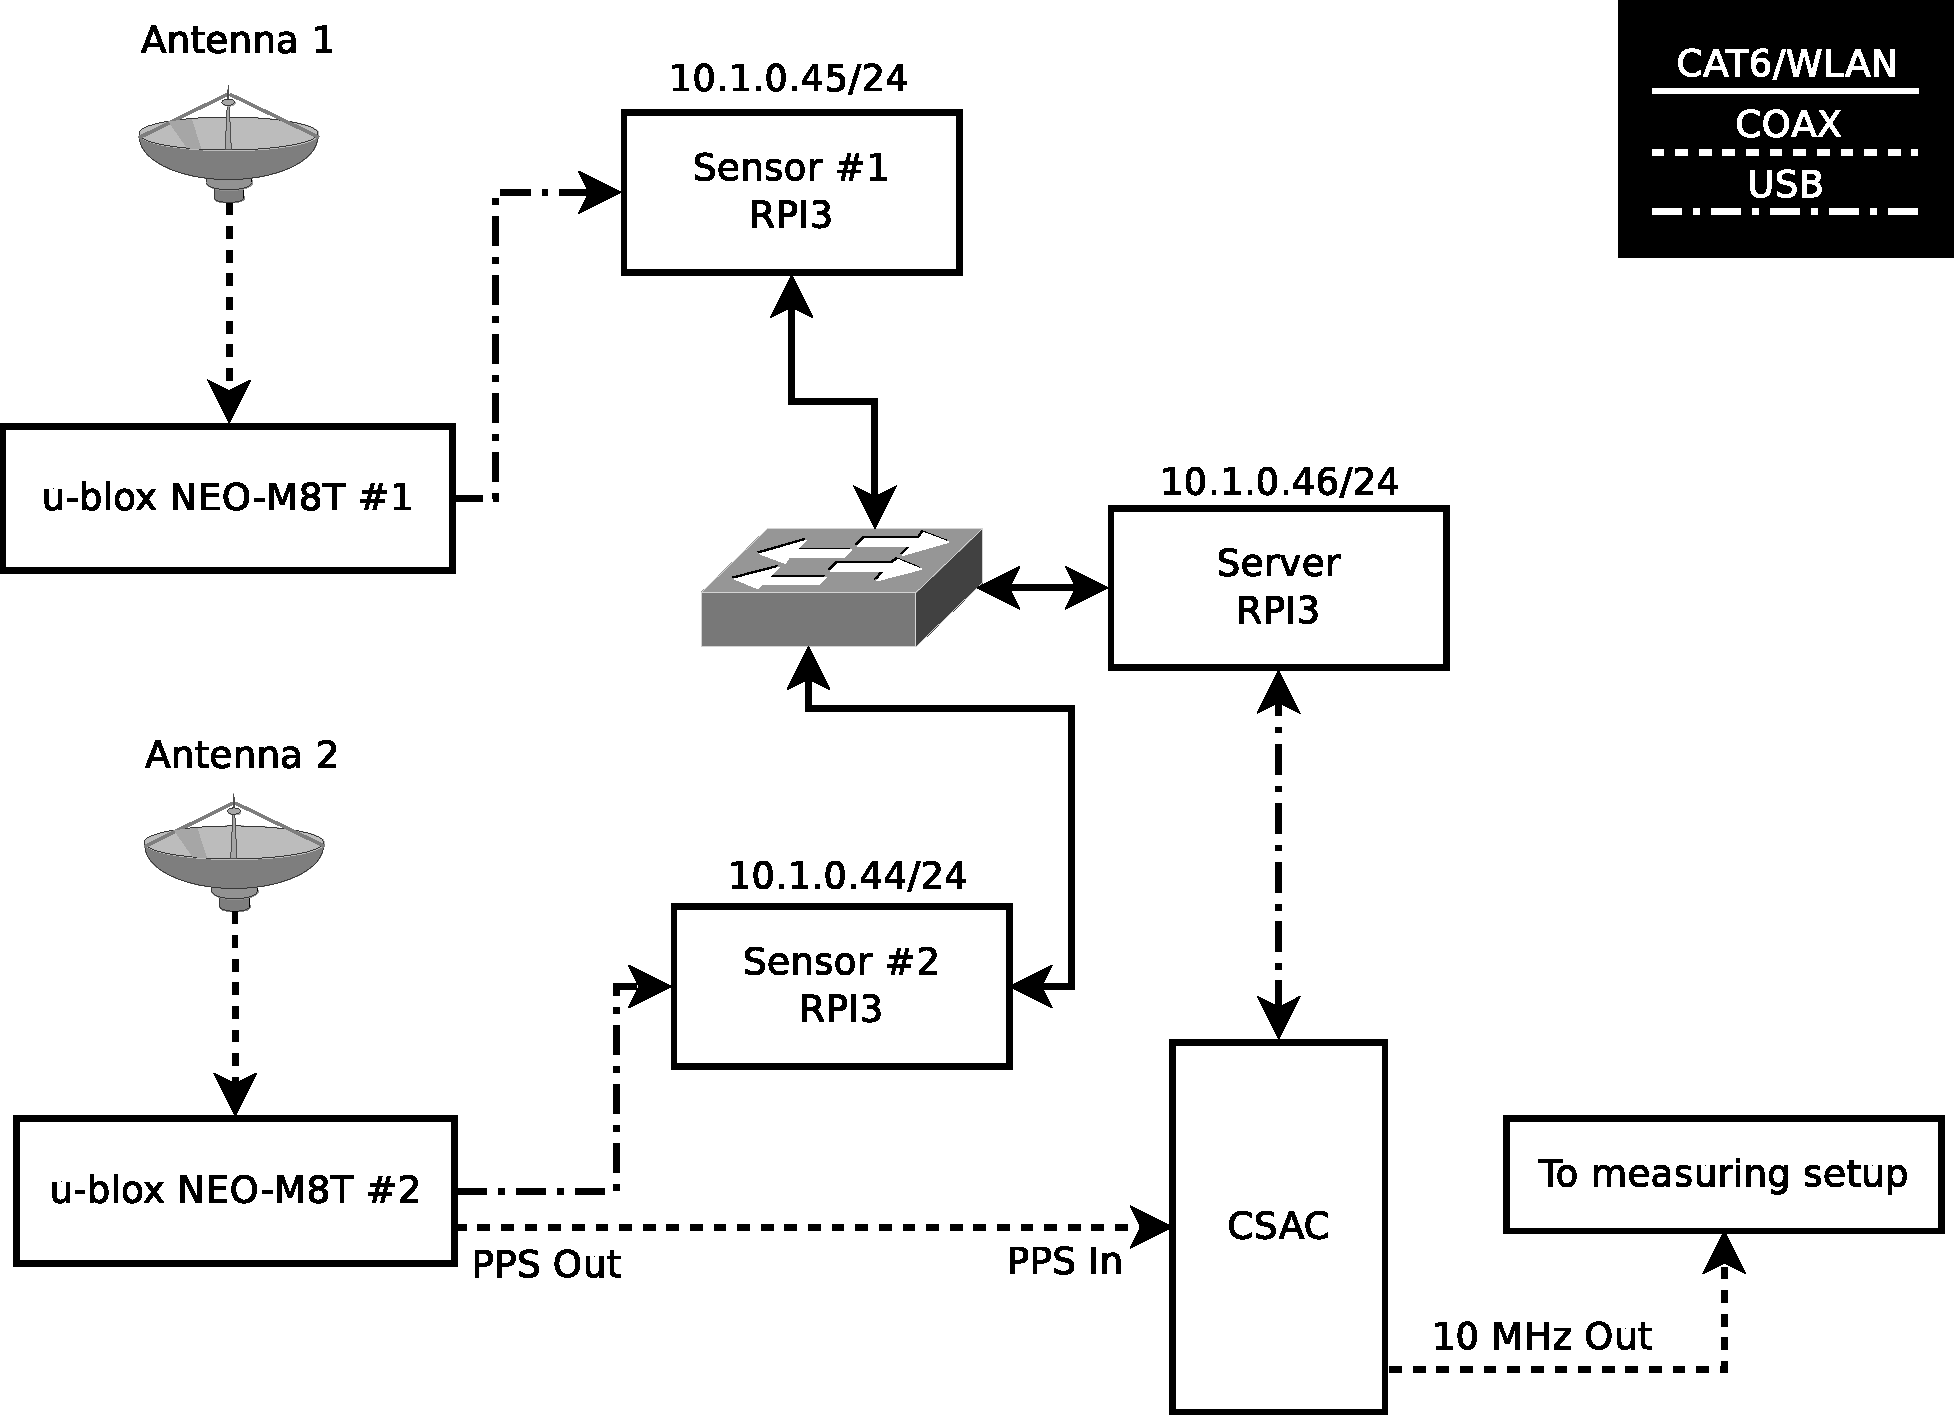
\includegraphics[scale=0.31]{server_layout_bw.pdf}
   \caption[atomic clock controller implementation block diagram]{A block diagram showing the tested implementation.}
   \label{ibd}
\end{figure}
Figure \ref{ibd} shows how the server, sensors and atomic clock were physically set up. In order to assure good GPS satellite geometry, the antennas were placed at the roof of Justervesenet's office at Kjeller. Antenna one was placed at a railing about one meter above the ground, antenna two was placed at ground level. Figure \ref{sensor_kart} shows the placement of the antennas. Antenna one was connected to GPS receiver one, which in turn was connected to sensor one. It was the same deal with antenna two, which was connected to GPS receiver two which in turn was connected to sensor two. The distance between the two antennas was about 35 meters. The antenna connected to sensor one was not placed as far away as the cable would have allowed. This is because it proved challenging to find a suitable place to securely place the antenna and at the same time use the full length of the cable. The sensors and the server were connected to a LAN through a Gigabit Ethernet switch. The server was configured to log telemetry data received from the atomic clock and the clients were configured to log all NMEA data received from their respective GPS receiver. GPS receiver two  supplied the atomic clock with a one PPS signal. Because the atomic clock model needs live data over time to mature, the system was started the 7 October 2016 and the test was performed 10 October 2016. Figure \ref{msd} is a block diagram showing how the measuring setup was physically configured. The measuring was done using a Spectracom CNT-91 frequency counter using a 10 MHz reference from Justervesenet's atomic clocks. The CNT-91 was configured to measure a continuous gap-less frequency at one second time-intervals. Figure \ref{lab_setup_photo} is a photograph of the measuring setup. Both sensors were configured to use Justervesenet's internal NTP server and to use UTC instead of GMT+1.

\section{Test one filter limits}
Table \ref{gps_filter_table} shows the filter thresholds used during test one. 

\begin{table}[!htb]
\centering
\caption{Filter thresholds used during test one. }
\label{gps_filter_table}
  \begin{tabular}{|l|l|l|}
  \hline
  \multicolumn{1}{|c|}{} & \multicolumn{1}{c|}{Sensor one} & \multicolumn{1}{c|}{Sensor two} \\ \hline
  Altitude reference                 & 123.8$^{\circ}$ & 122.427$^{\circ}$                       \\ \hline
  Longitude reference                & 1102.1948$^{\circ}$ & 1102.1934$^{\circ}$                     \\ \hline
  Latitude reference                 & 5958.5448$^{\circ}$ & 5958.5231$^{\circ}$                     \\ \hline
  Speed reference                    & 0 knot        & 0 knot                            \\ \hline
  Altitude deviation                 & 10$^{\circ}$        & 10$^{\circ}$                            \\ \hline
  Longitude deviation                & 0.005$^{\circ}$     & 0.005$^{\circ}$                         \\ \hline
  Latitude deviation                 & 0.005$^{\circ}$     & 0.005$^{\circ}$                         \\ \hline
  Speed deviation                    & 10 knot        & 10 knot                             \\ \hline
  \end{tabular}
\end{table} 

\begin{figure}[!htb]
\centering
  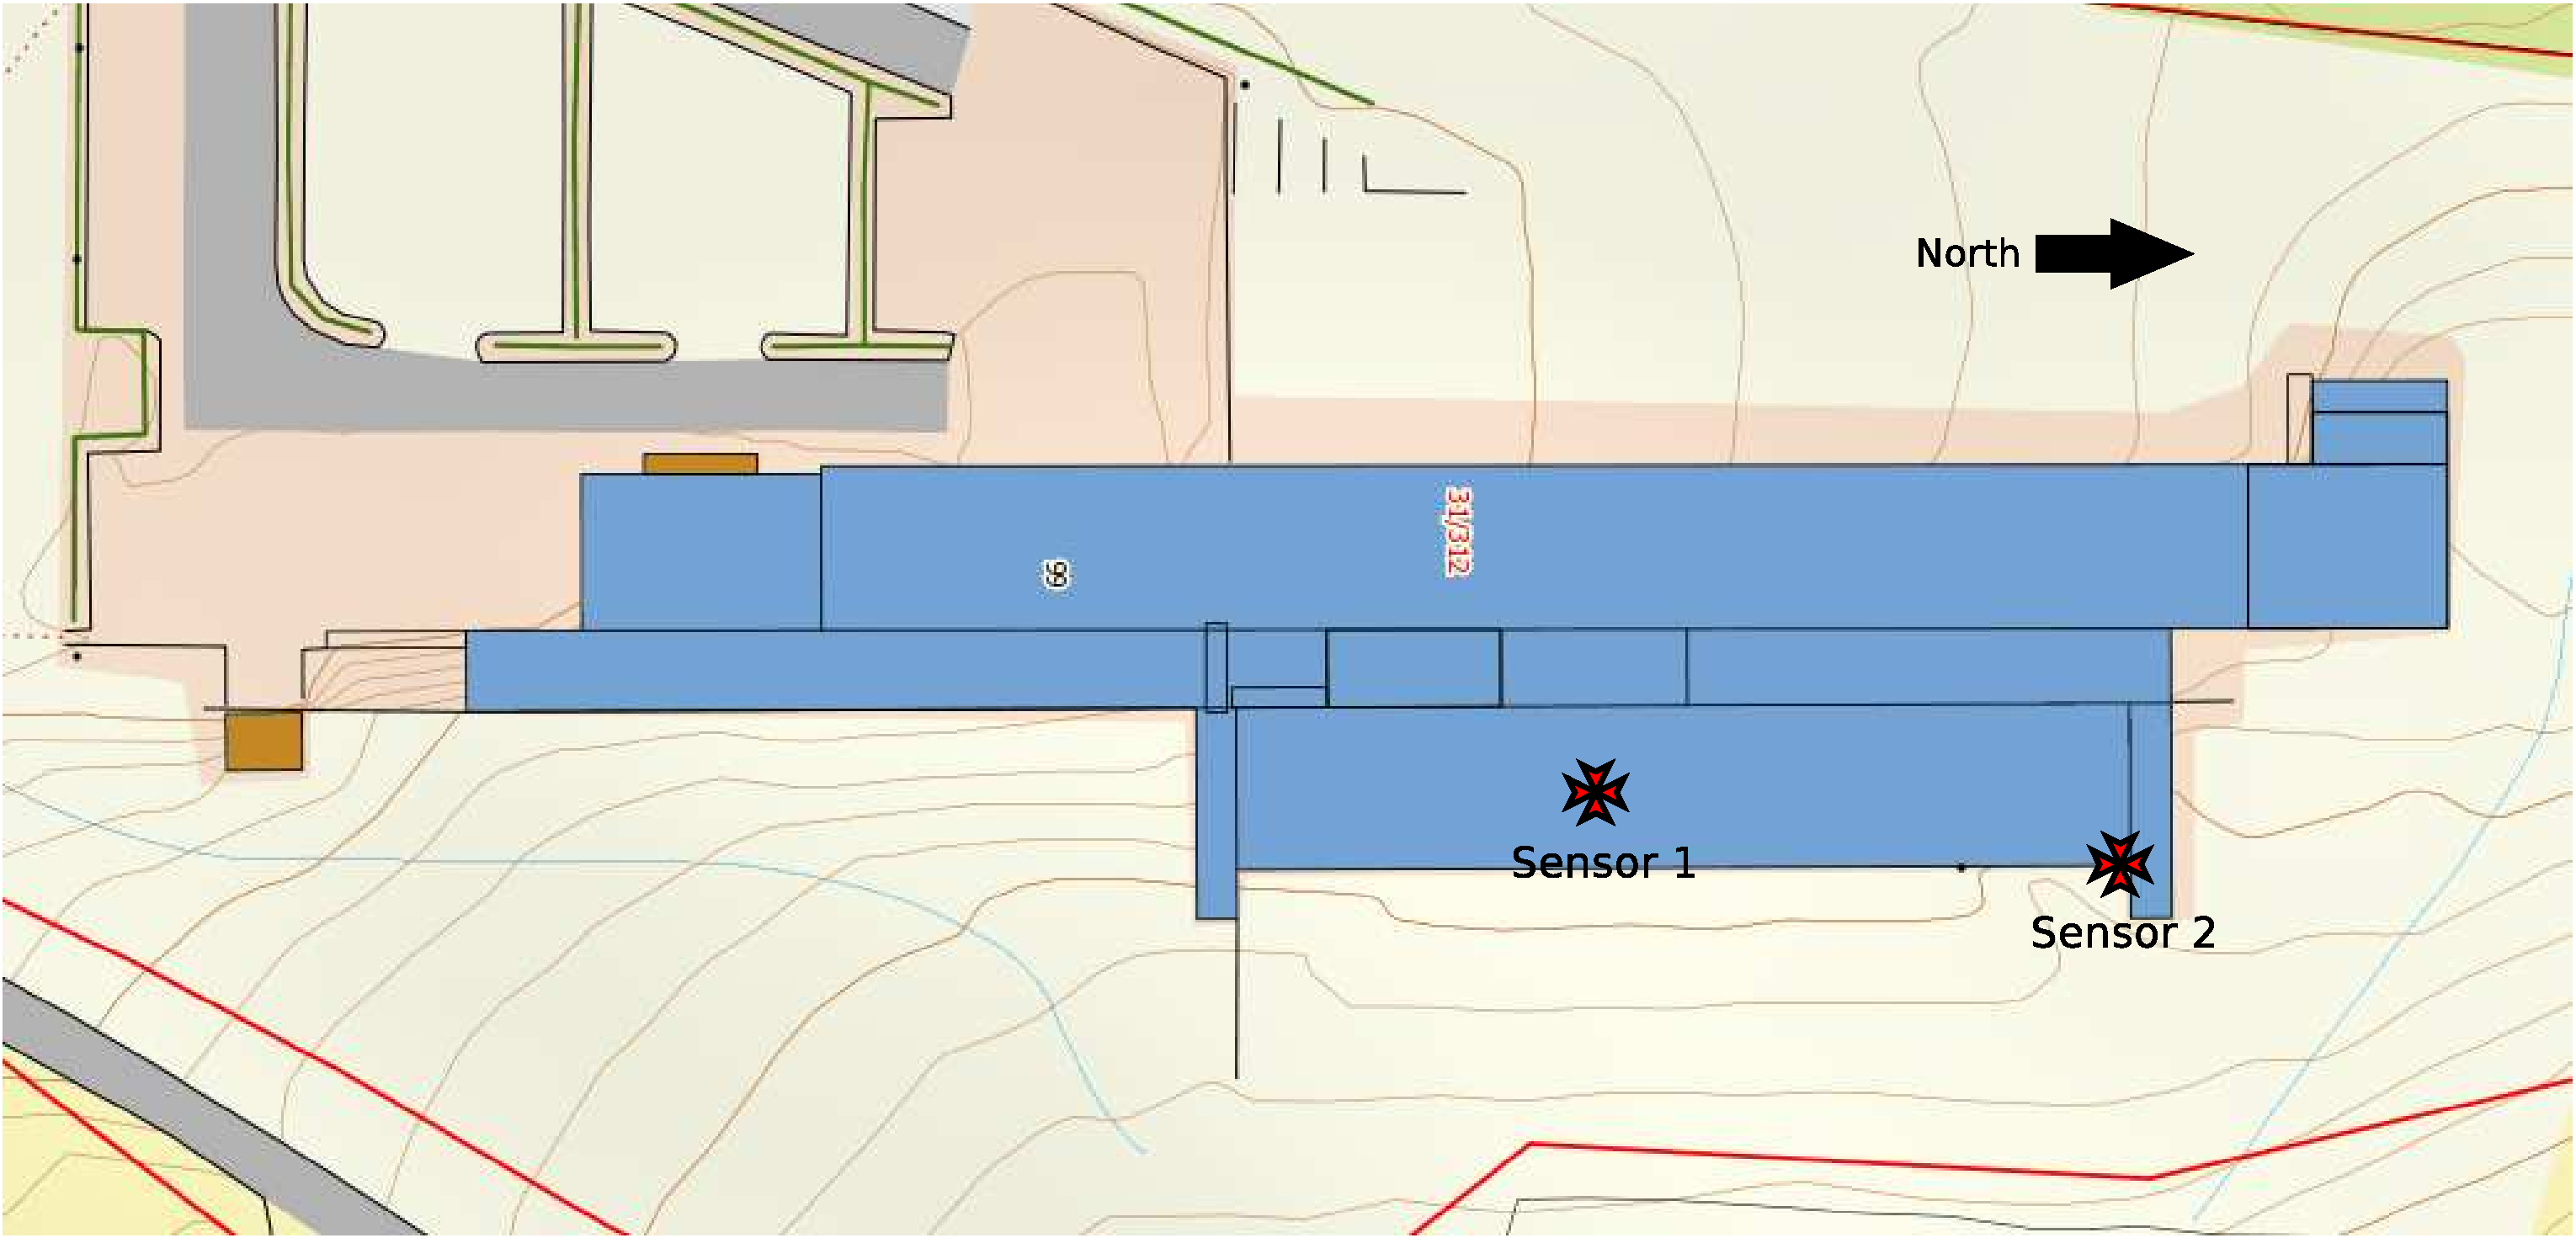
\includegraphics[scale=0.25]{roof.pdf}
   \caption[Measurement setup]{Block diagram showing the position of the antennas as reported by the receivers. Map courtesy of Kartverket \cite{KART}}
   \label{sensor_kart}
\end{figure}

\begin{figure}[!htb]
\centering
  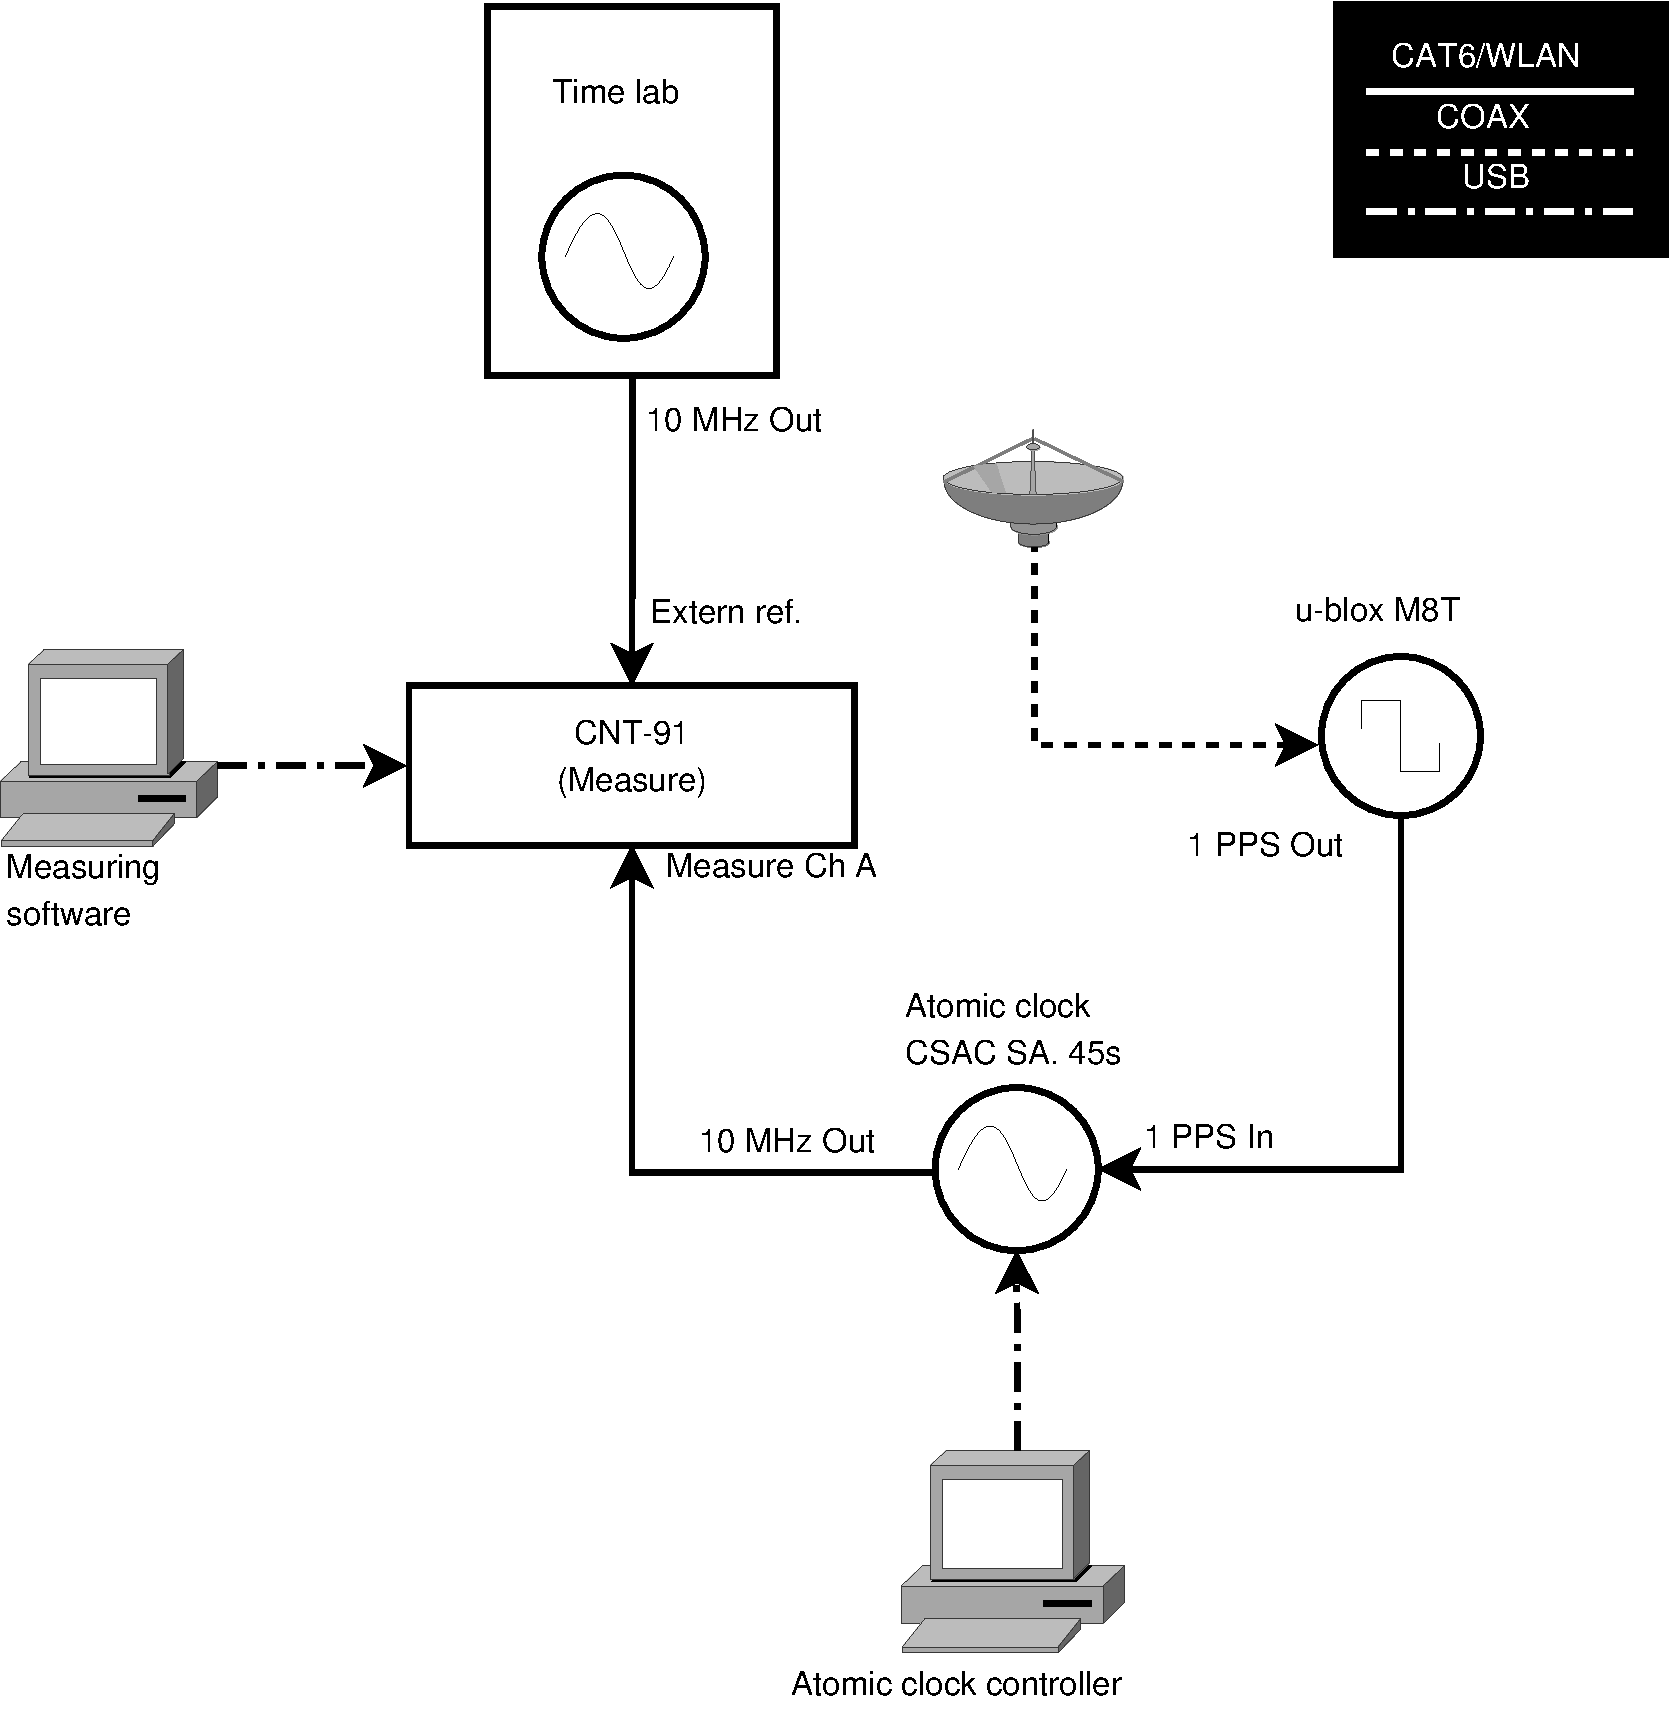
\includegraphics[scale=0.4]{measure_setup_bw.pdf}
   \caption[Measurement setup]{Block diagram showing the setup of the measurement equipment}
   \label{msd}
\end{figure}

\section{Test one}
\subsection{Goal of test one}
The goal with test one was to use the atomic clock controller to detect a simulated spoofing attack. By moving the antennas, the location and speed filter should be triggered as the solved longitude, altitude, latitude and speed change. See section \ref{ls_filter} for more about the location and speed filter. The result is observable by analyzing the log files produced by the server and clients and the data collected by the measuring setup.

\subsection{Description}\label{test1_description}
The following is a step by step description of how the test was conducted. The time in the brackets was obtained from a wristwatch. The time is written in the normal format (hours and minutes) as well as number of seconds after 10:48. This is because the data used to draw the graphs started at 10:48 but uses seconds on the x-axis, to ease comparison. It is important to note that neither the resolution nor the accuracy was of any notable concern when the time was noted down. The time was mainly noted to make it easier to find any correlation between the steps taken and patterns found in the log files. 

\begin{itemize}
  \item\relax 10:58 - 600: Moved antenna 1 approximately 15 meters to the south.
  \item\relax 11:03 - 900: Moved antenna 1 back to original location.
  \item\relax 11:07 - 1140: Moved antenna 2 approximately 15 meters to the north.
  \item\relax 11:12 - 1440: Moved antenna 2 back to original location.
  \item\relax 11:14 - 1560: Waved antenna 1 around horizontally in a half circle motion at an increasing tempo.
  \item\relax 11:18 - 1800: Waved antenna 2 around horizontally in a half circle motion at an increasing tempo.
  \item\relax 11:20 - 1920: Covered antenna 1 with aluminium foil.
  \item\relax 11:25 - 2220: Covered antenna 2 with aluminium foil.
  \item\relax 11:28 - 2400: Removed foil from antenna 1.
  \item\relax 11:33 - 2700: Removed foil from antenna 2.
\end{itemize}

Step one and two were designed to trigger the location and speed filter, especially the check of solved latitude, longitude and altitude but also the speed against known values. Step five and six were also designed to trigger the location and speed filter but more specifically the checking of solved speed. By waving the antenna around while standing still, the solved location should not exceed the configured limits except for speed. Step seven and eight were designed to reveal what would happen during a jamming attack as it was believed that covering the antennas with aluminium foil would block all signals out. A photography showing how the antenna was covered with aluminium foil can be seen in section \ref{antenna_foil_cover} in the appendix.

\subsection{Observations}\label{test1_observations}
\subsubsection{Sensor Server logs}
By reviewing the log produced by the server, the following was observed:

\begin{itemize}
  \item No false positives were reported. The filters were not triggered before the test started.
  \item The location and speed filter was triggered by sensor one at 10:59:19 and cleared at 11:04:35.
  \begin{lstlisting}
    [10/10/16 - 10:59:17] [ ALARM ] Sensor 1 triggered LS filter!
    ...
    [10/10/16 - 11:04:35] [ ALARM ] Sensor 1 cleared LS filter!
  \end{lstlisting}
  \item The location and speed filter was triggered again at 11:08:27, but this time by sensor one. The alarm was cleared at 11:13:43.
    \begin{lstlisting}
    [10/10/16 - 11:08:27] [ ALARM ] Sensor 2 triggered LS filter!
    ...
    [10/10/16 - 11:13:43] [ ALARM ] Sensor 2 cleared LS filter!
  \end{lstlisting}
  \item Once again, 11:22:03 the location and speed filter was triggered by sensor one and was not cleared until 11:29:21
     \begin{lstlisting}
    [10/10/16 - 11:22:03] [ ALARM ] Sensor 1 triggered LS filter!
    ...
    [10/10/16 - 11:29:21] [ ALARM ] Sensor 1 cleared LS filter!
  \end{lstlisting} 
  \item Sensor two triggered the location and speed filter 11:27:31 and cleared at 11:34:16.
    \begin{lstlisting}
    [10/10/16 - 11:27:31] [ ALARM ] Sensor 2 triggered LS filter!
    [10/10/16 - 11:34:16] [ ALARM ] Sensor 2 cleared LS filter!
  \end{lstlisting} 
  \item The last three seconds, sensor two triggered and cleared the location and speed filter.
  \begin{lstlisting}
    [10/10/16 - 11:34:17] [ ALARM ] Sensor 2 triggered LS filter!
    [10/10/16 - 11:34:20] [ ALARM ] Sensor 2 cleared LS filter!
  \end{lstlisting} 
\end{itemize}

\subsubsection{GPS data}\label{gpsdata_test1}
The figures in this section are plots of the GPS data that was logged by the sensors during test one. Figure \ref{sensor1_alt} shows the altitude in meters reported by sensor one. The only thing that stands out in the plot is when the antenna is covered in aluminium foil as shown at around the 2000 second mark. At this point the receiver is no longer able to solve for a position thus generating valid but empty fields in the NMEA data. This creates a deep void in the plot. Because both receivers' antennas were covered in aluminium foil, the plots all share this trait. Figure \ref{sensor2_alt} shows the altitude in meters as reported by sensor two. When compared with the altitude plot for sensor one \ref{sensor1_alt}, sensor one seems to correlate better. It remains a puzzle why sensor two reported to have been moved seven meters down which it clearly was not. When examining figures \ref{sensor1_lat} and \ref{sensor2_lat} showing the latitude for sensor one and two (in that order), one can clearly see that sensor one was moved to the south and sensor two was moved to the north. One might also notice that sensor two traveled further. The difference in travel is because sensor one's cable is shorter. This is explained in the description of test one. Figures \ref{sensor1_long} and \ref{sensor2_long} shows a plot for the solved longitude for sensor one and two. When examining figure \ref{sensor1_long}, it seems as if the antenna were never moved. This is because the building the antenna was placed on is position in a north to south line and the receiver was moved along with the roof. The antenna connected to sensor two was not moved in straight line because the cable got caught in vegetation. The last two figures, figure \ref{sensor1_speed} and figure \ref{sensor2_speed} show the speed solved by sensor one and two. They both correlate well with when the antennas were moved. However, the antenna connected to sensor two seems to be slightly more sensitive than the antenna connected to sensor one.

\begin{sidewaysfigure}
  \centering
  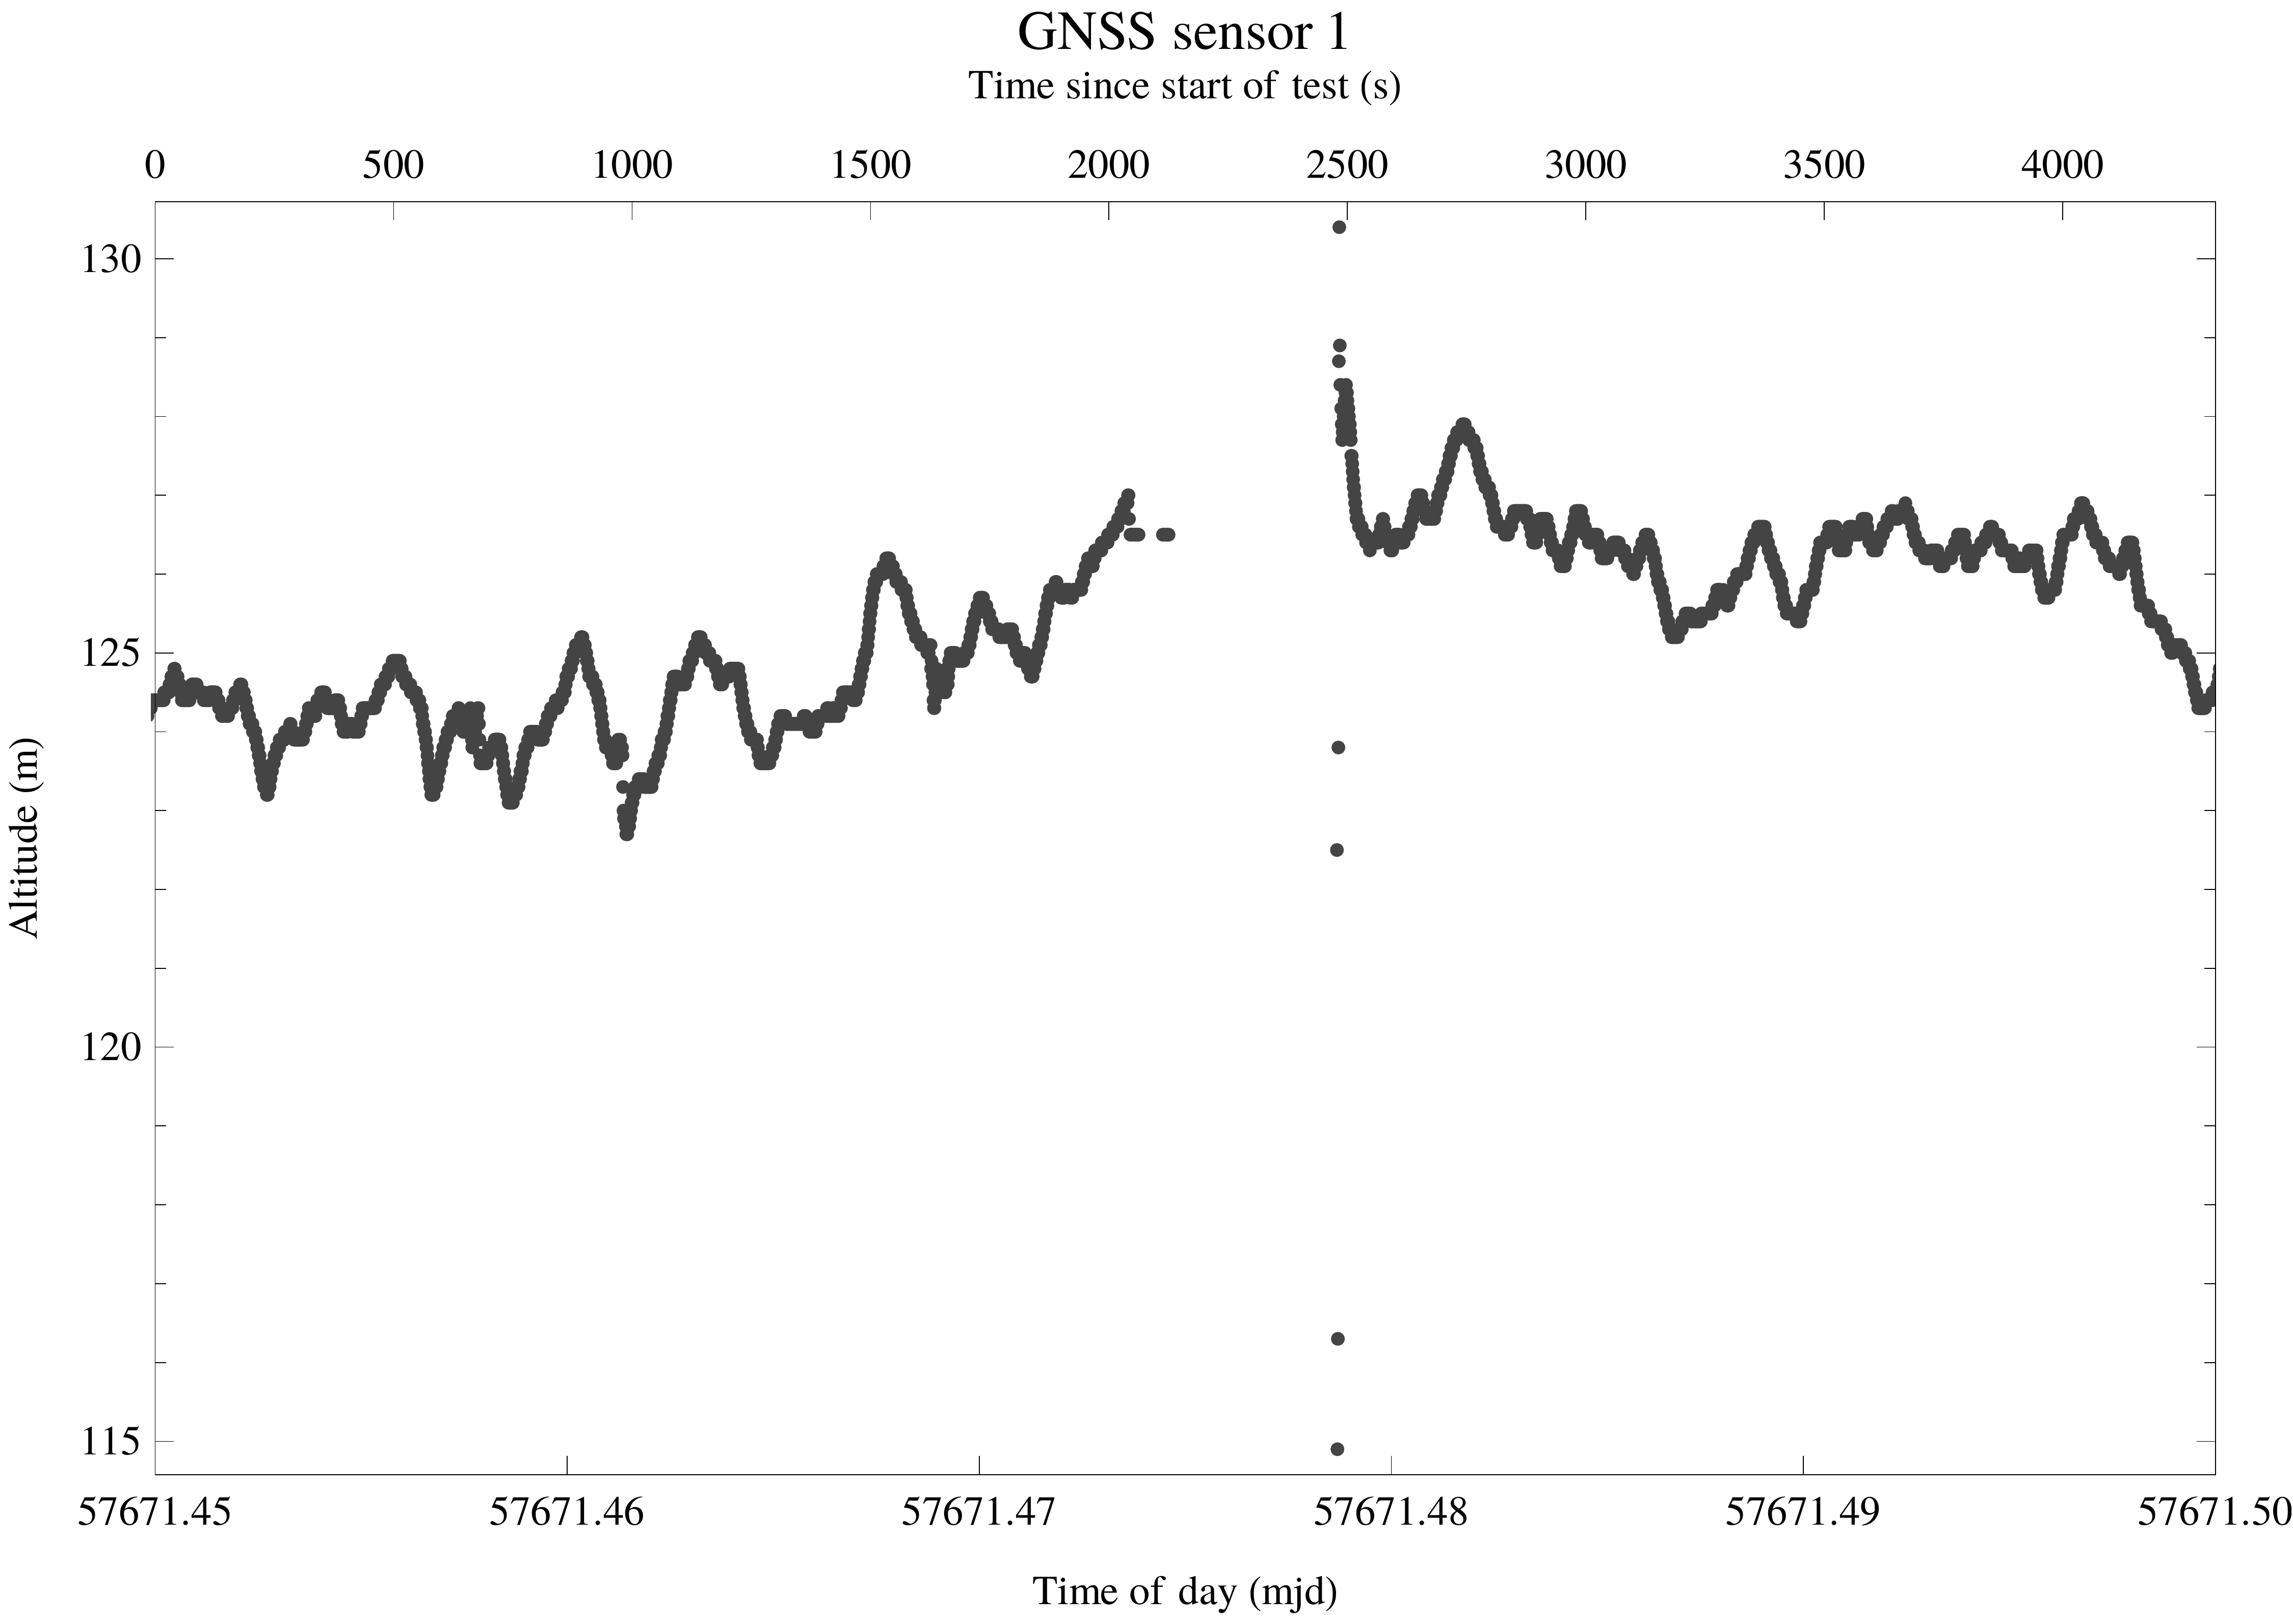
\includegraphics[width=1\textwidth]{gnssAlt1-1g.png}
  \caption{The figure shows the solved altitude of the GPS receiver connected to sensor one, during test one}
  \label{sensor1_alt}
\end{sidewaysfigure}

\begin{sidewaysfigure}
  \centering
  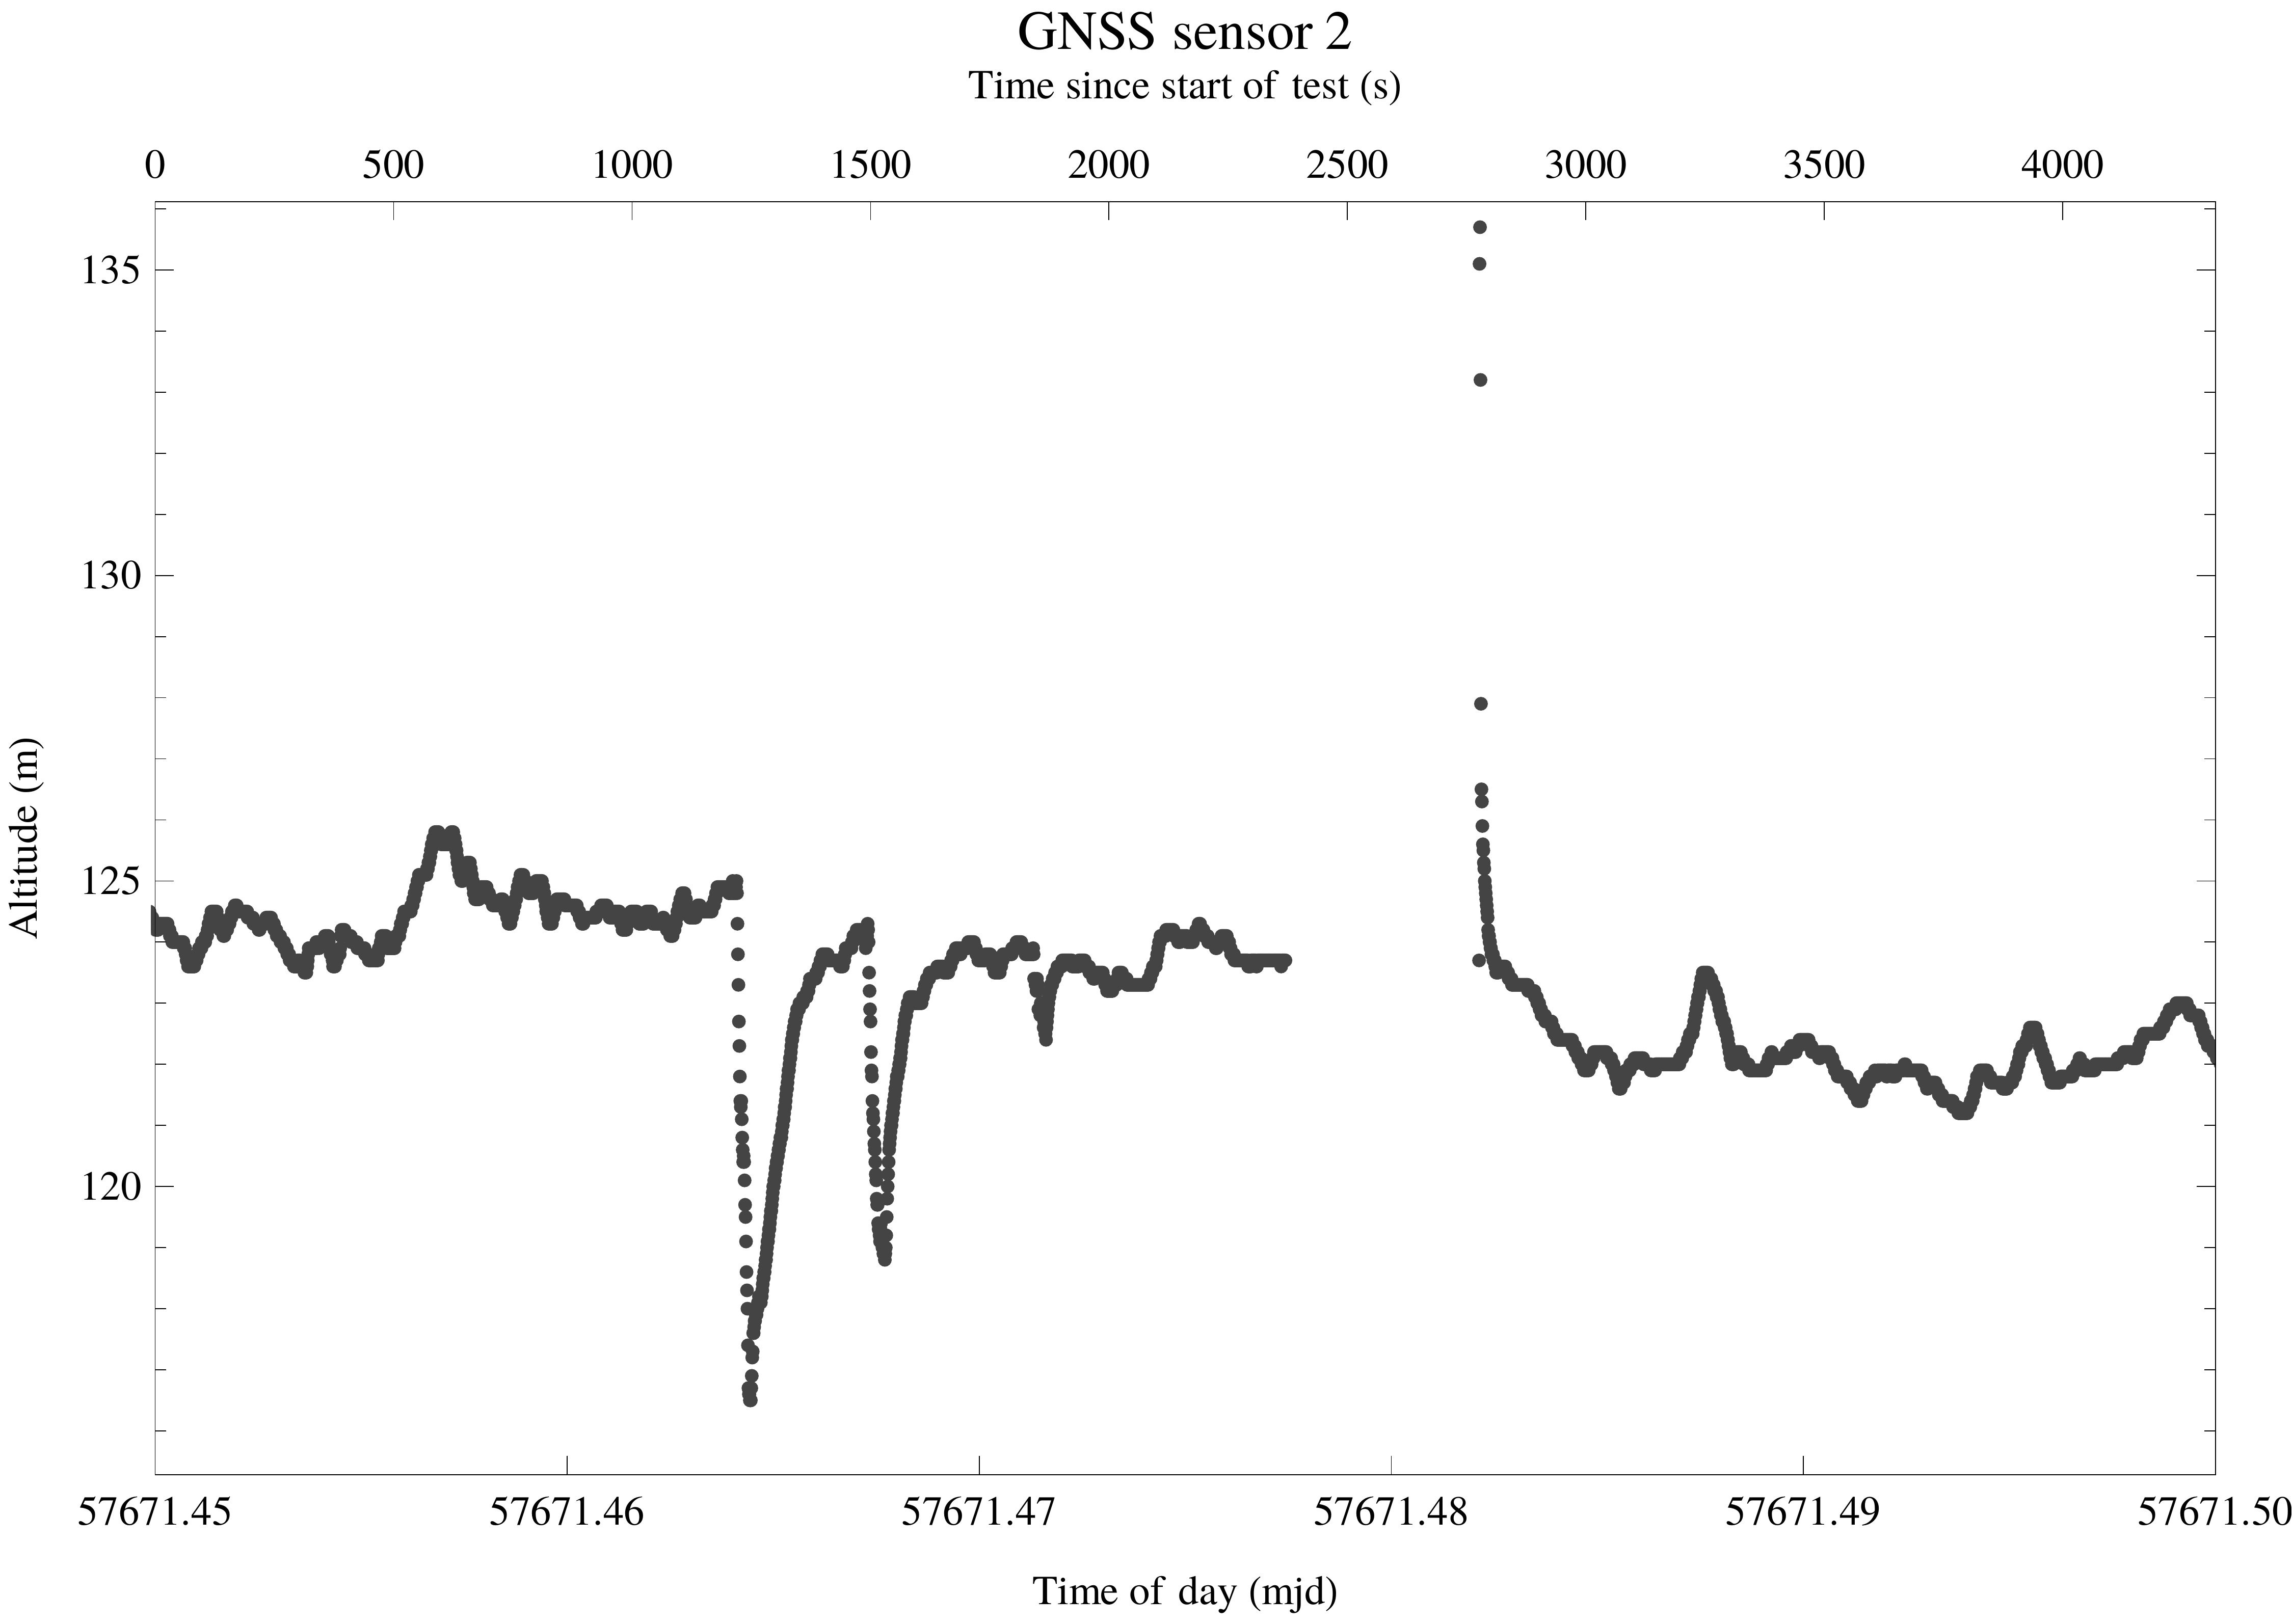
\includegraphics[width=1\textwidth]{gnssAlt2-1g.png}
  \caption{The figure shows the solved altitude of the GPS receiver connected to sensor two, during test one}
  \label{sensor2_alt}
\end{sidewaysfigure}

\begin{sidewaysfigure}
  \centering
  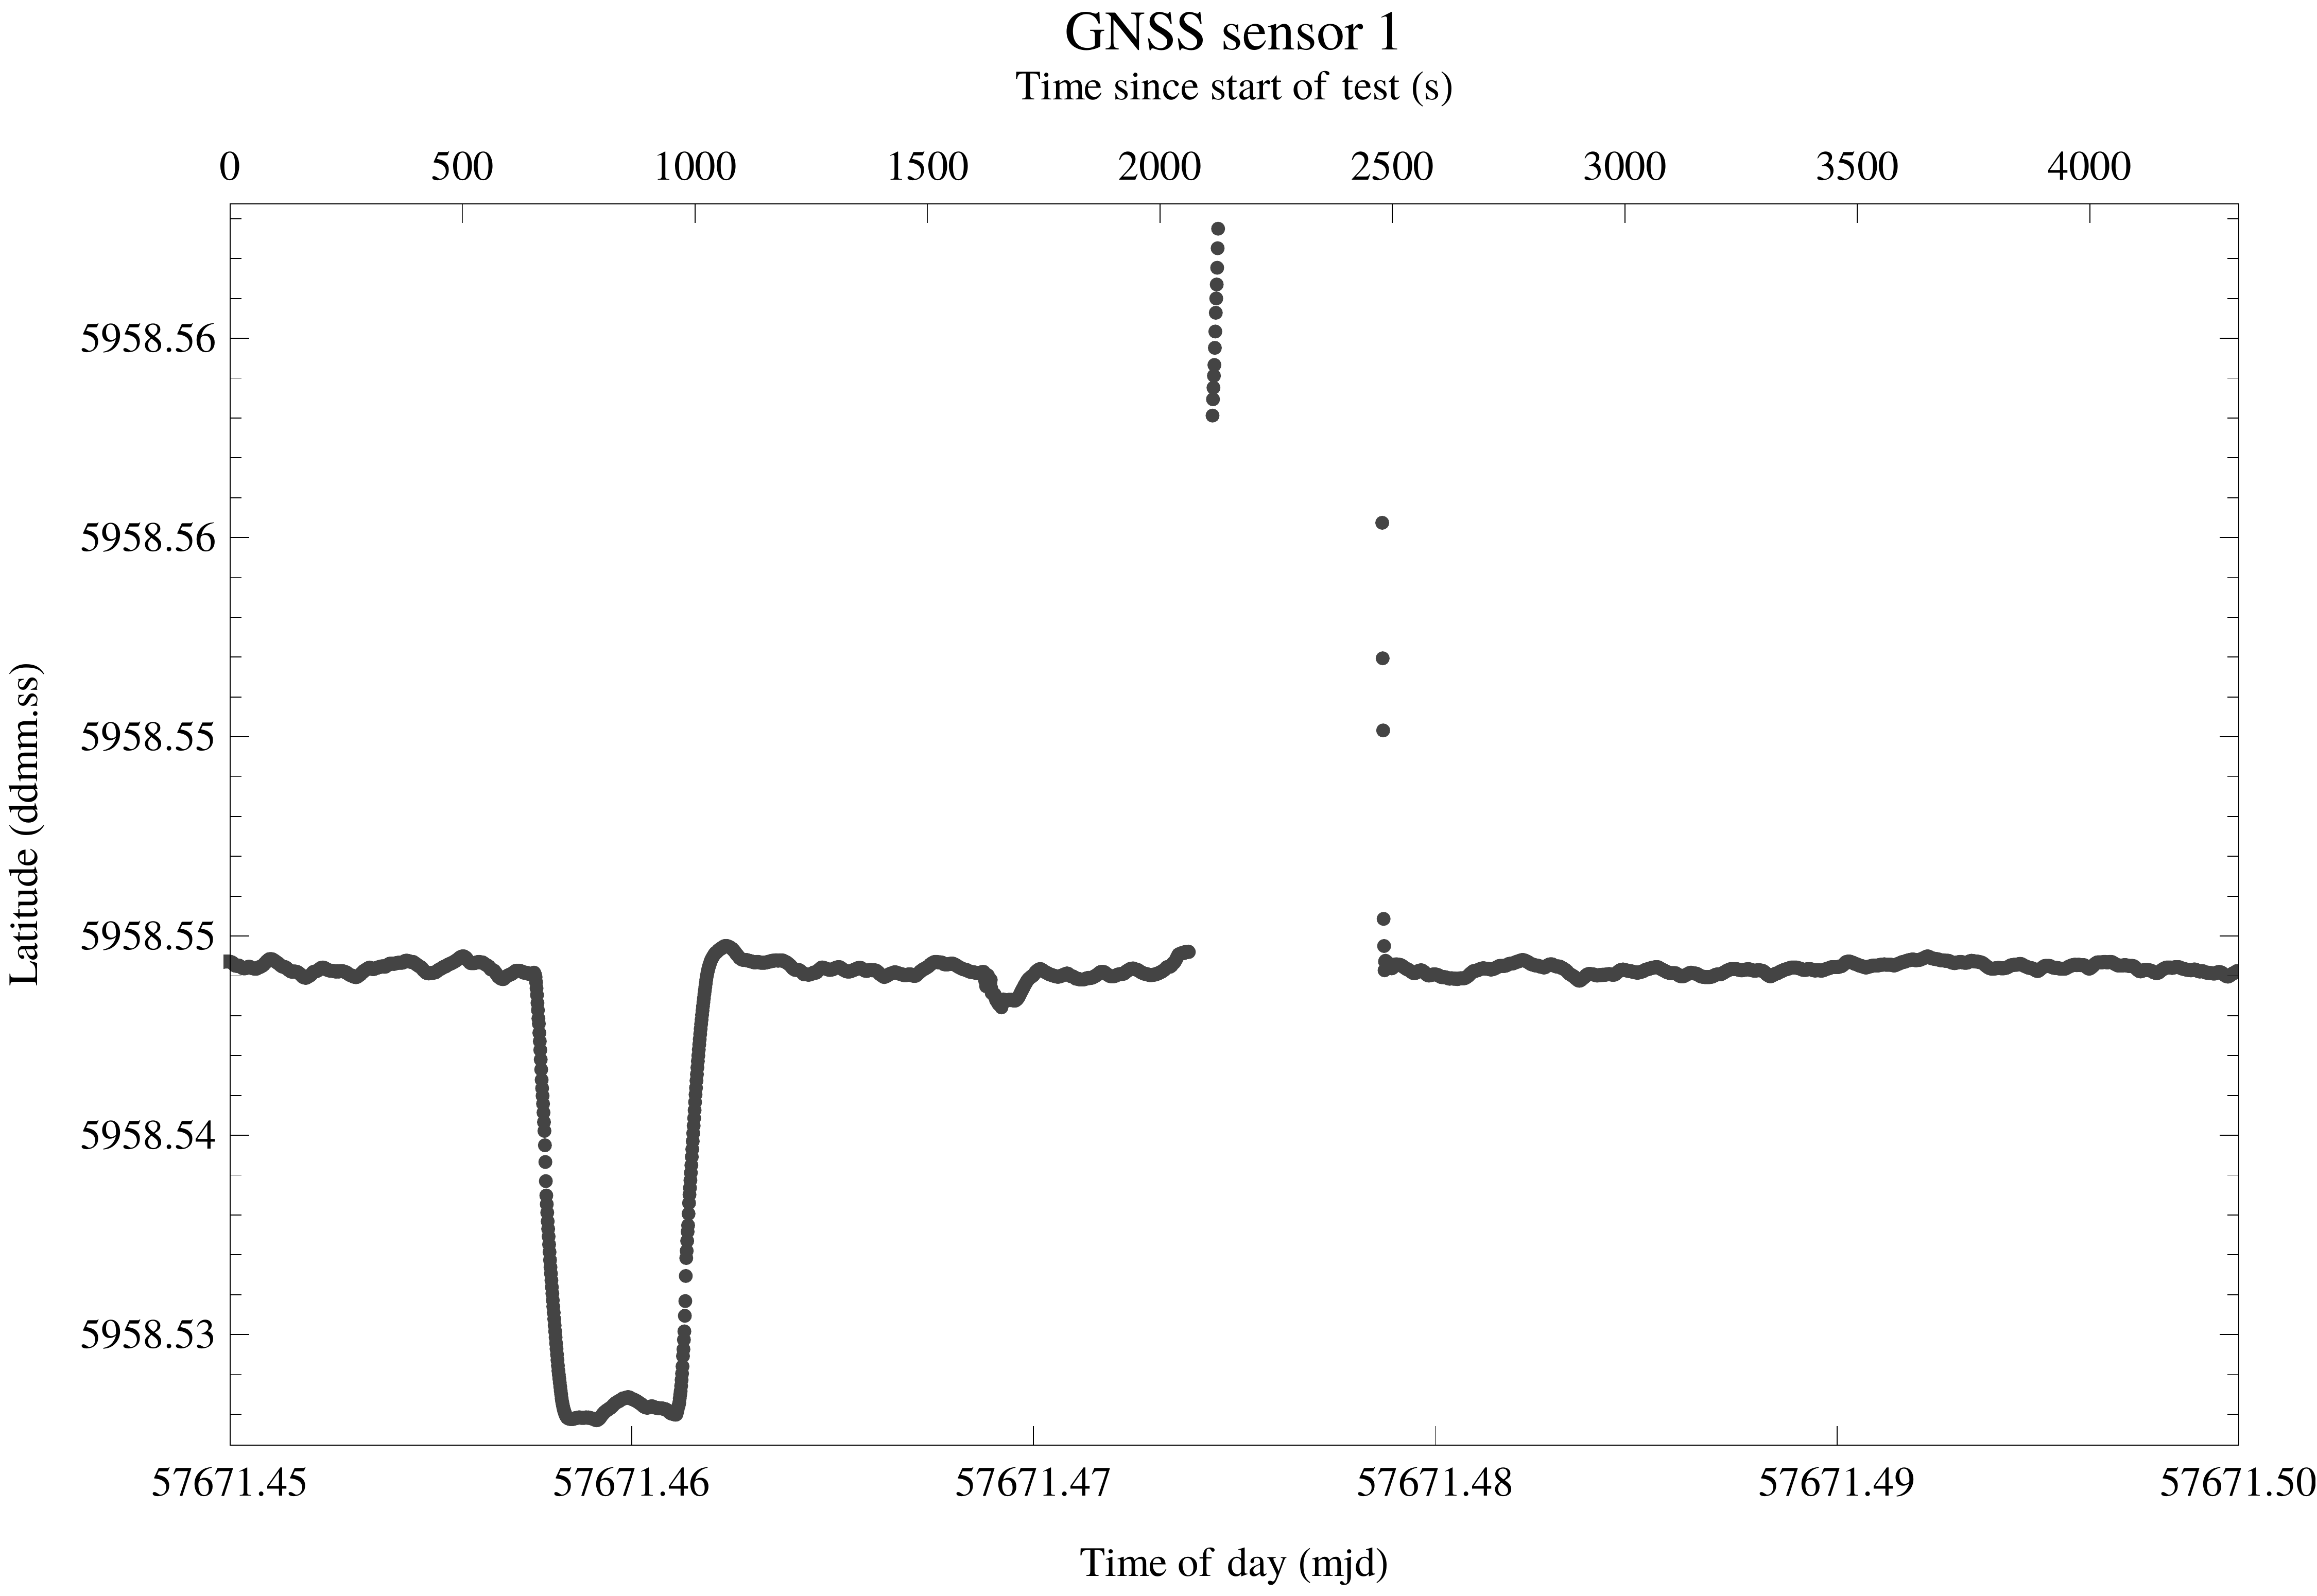
\includegraphics[width=1\textwidth]{gnssLat1-1g.png}
  \caption{The figure shows the solved latitude of the GPS receiver connected to sensor one, during test one}
  \label{sensor1_lat}
\end{sidewaysfigure}
 

\begin{sidewaysfigure}
  \centering
  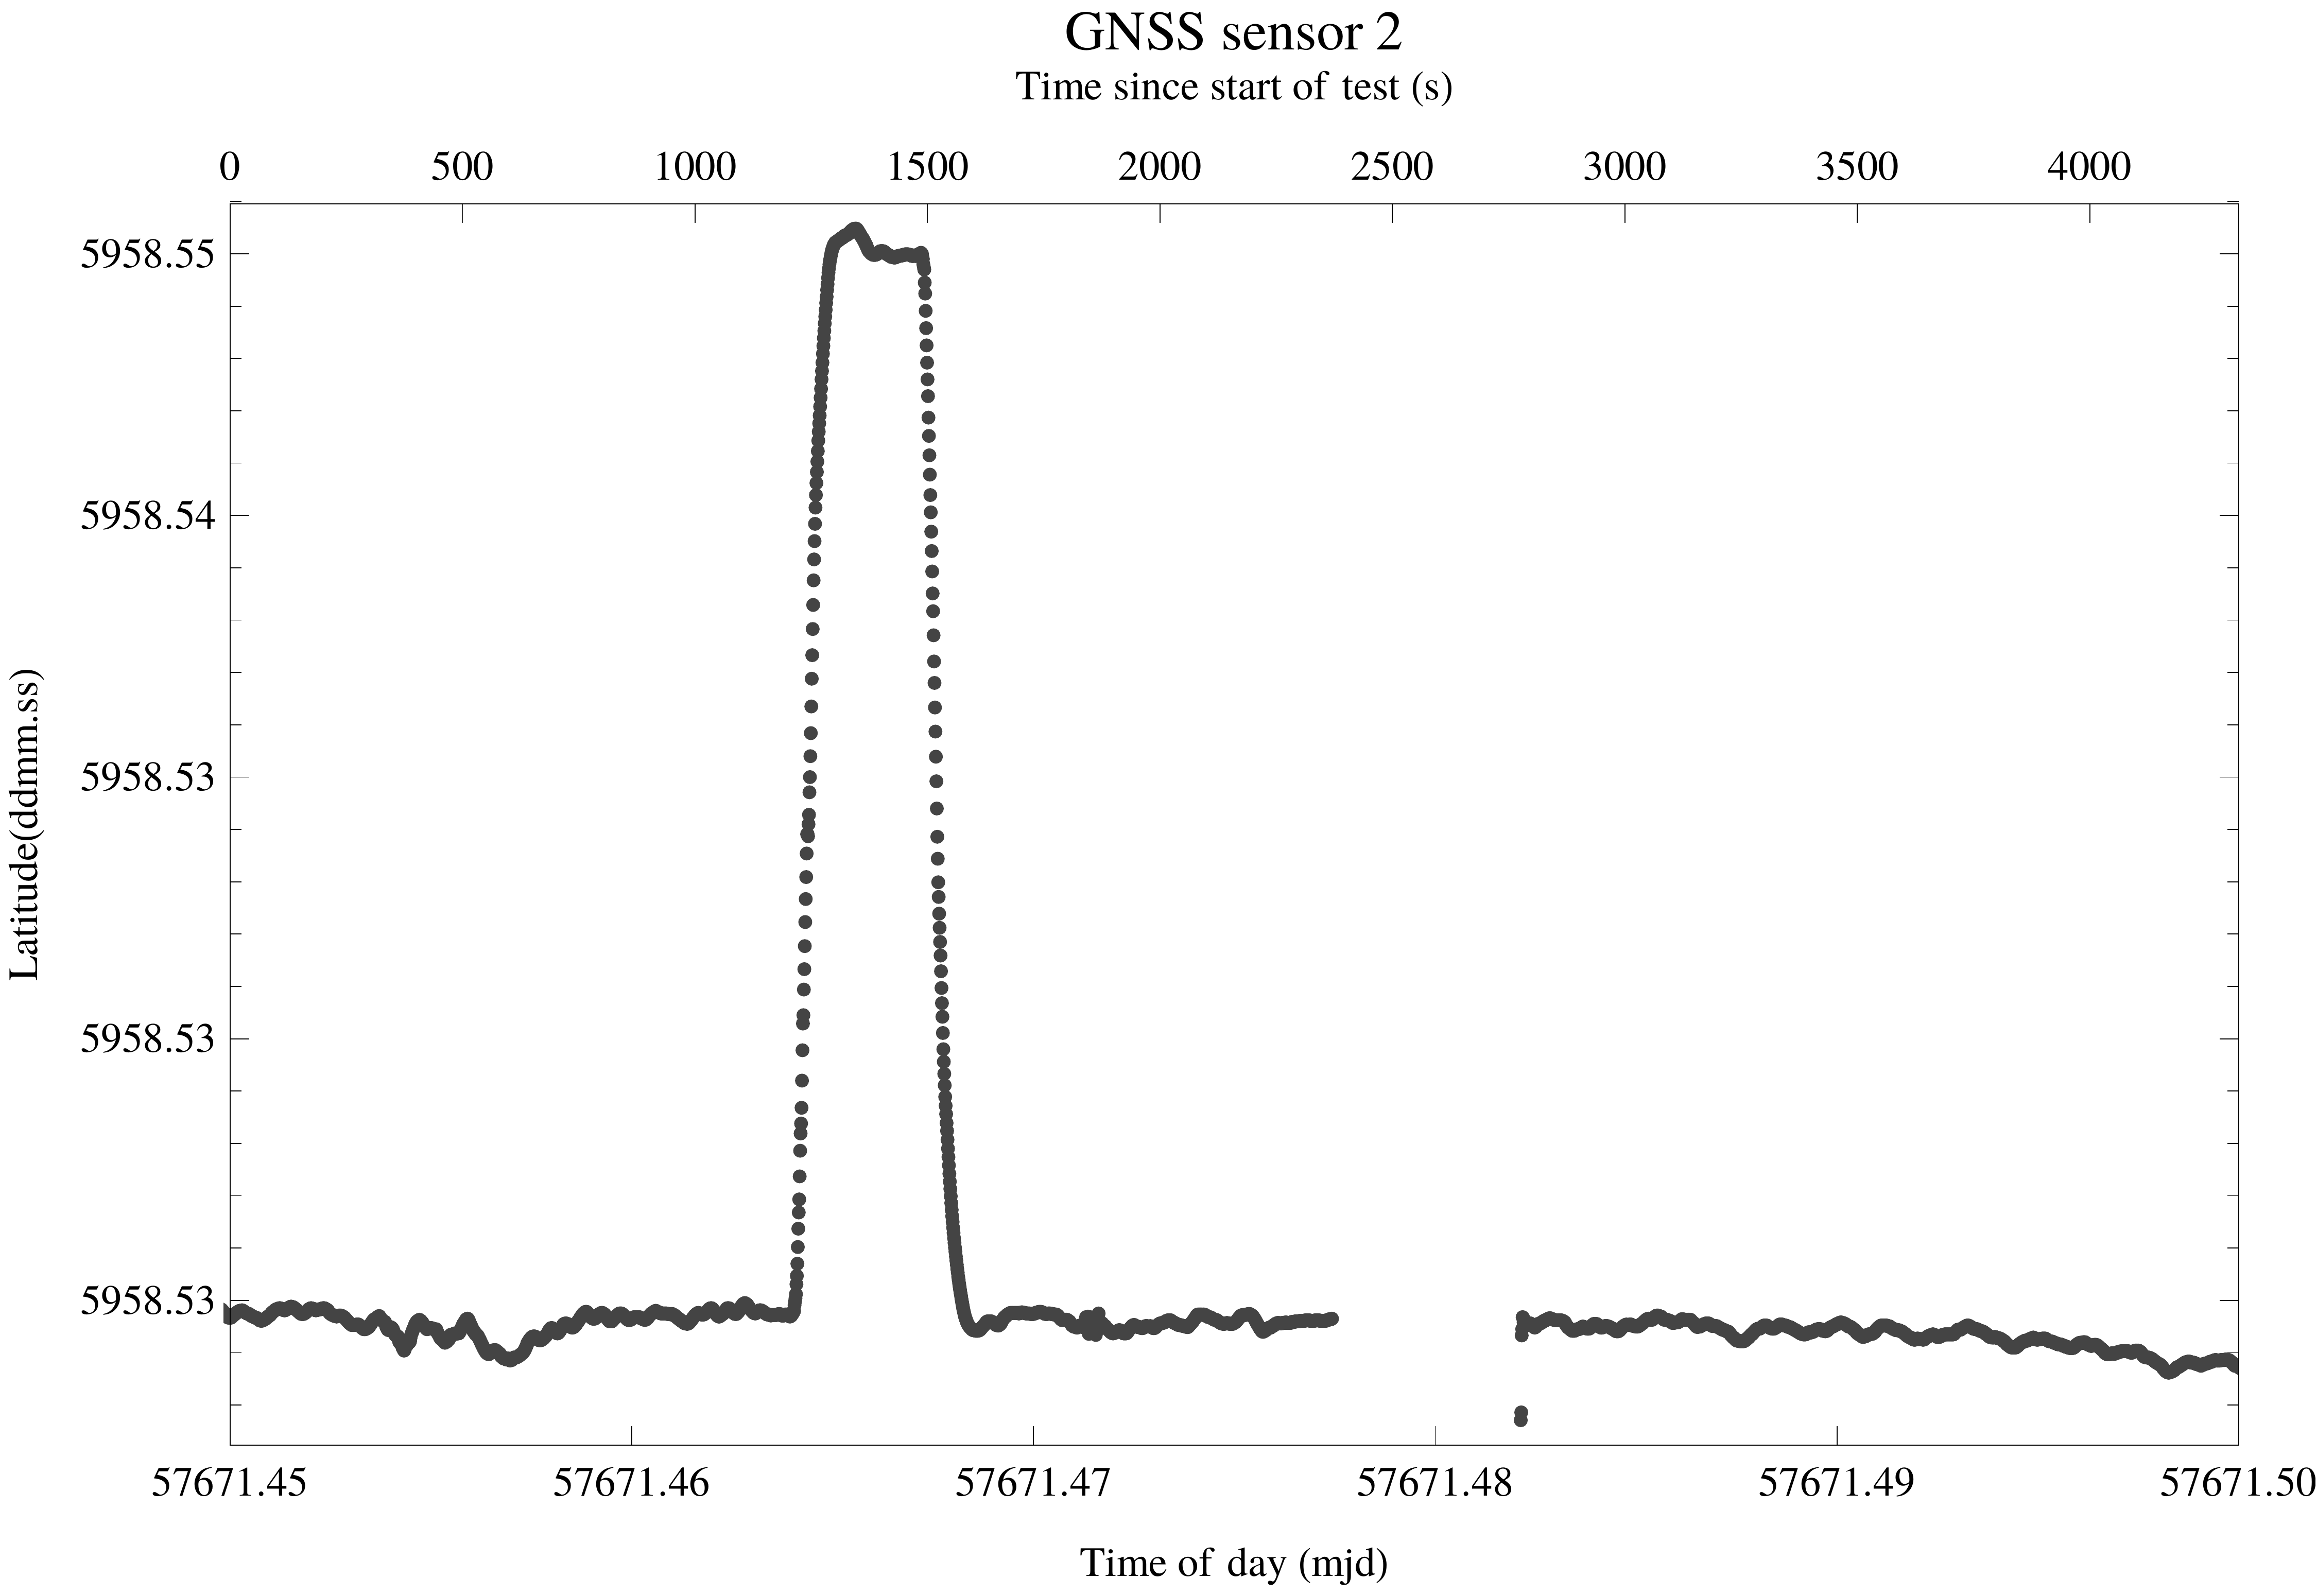
\includegraphics[width=1\textwidth]{gnssLat2-1g.png}
  \caption{The figure shows the solved latitude of the GPS receiver connected to sensor two, during test one}
  \label{sensor2_lat}
\end{sidewaysfigure}
 

\begin{sidewaysfigure}
  \centering
  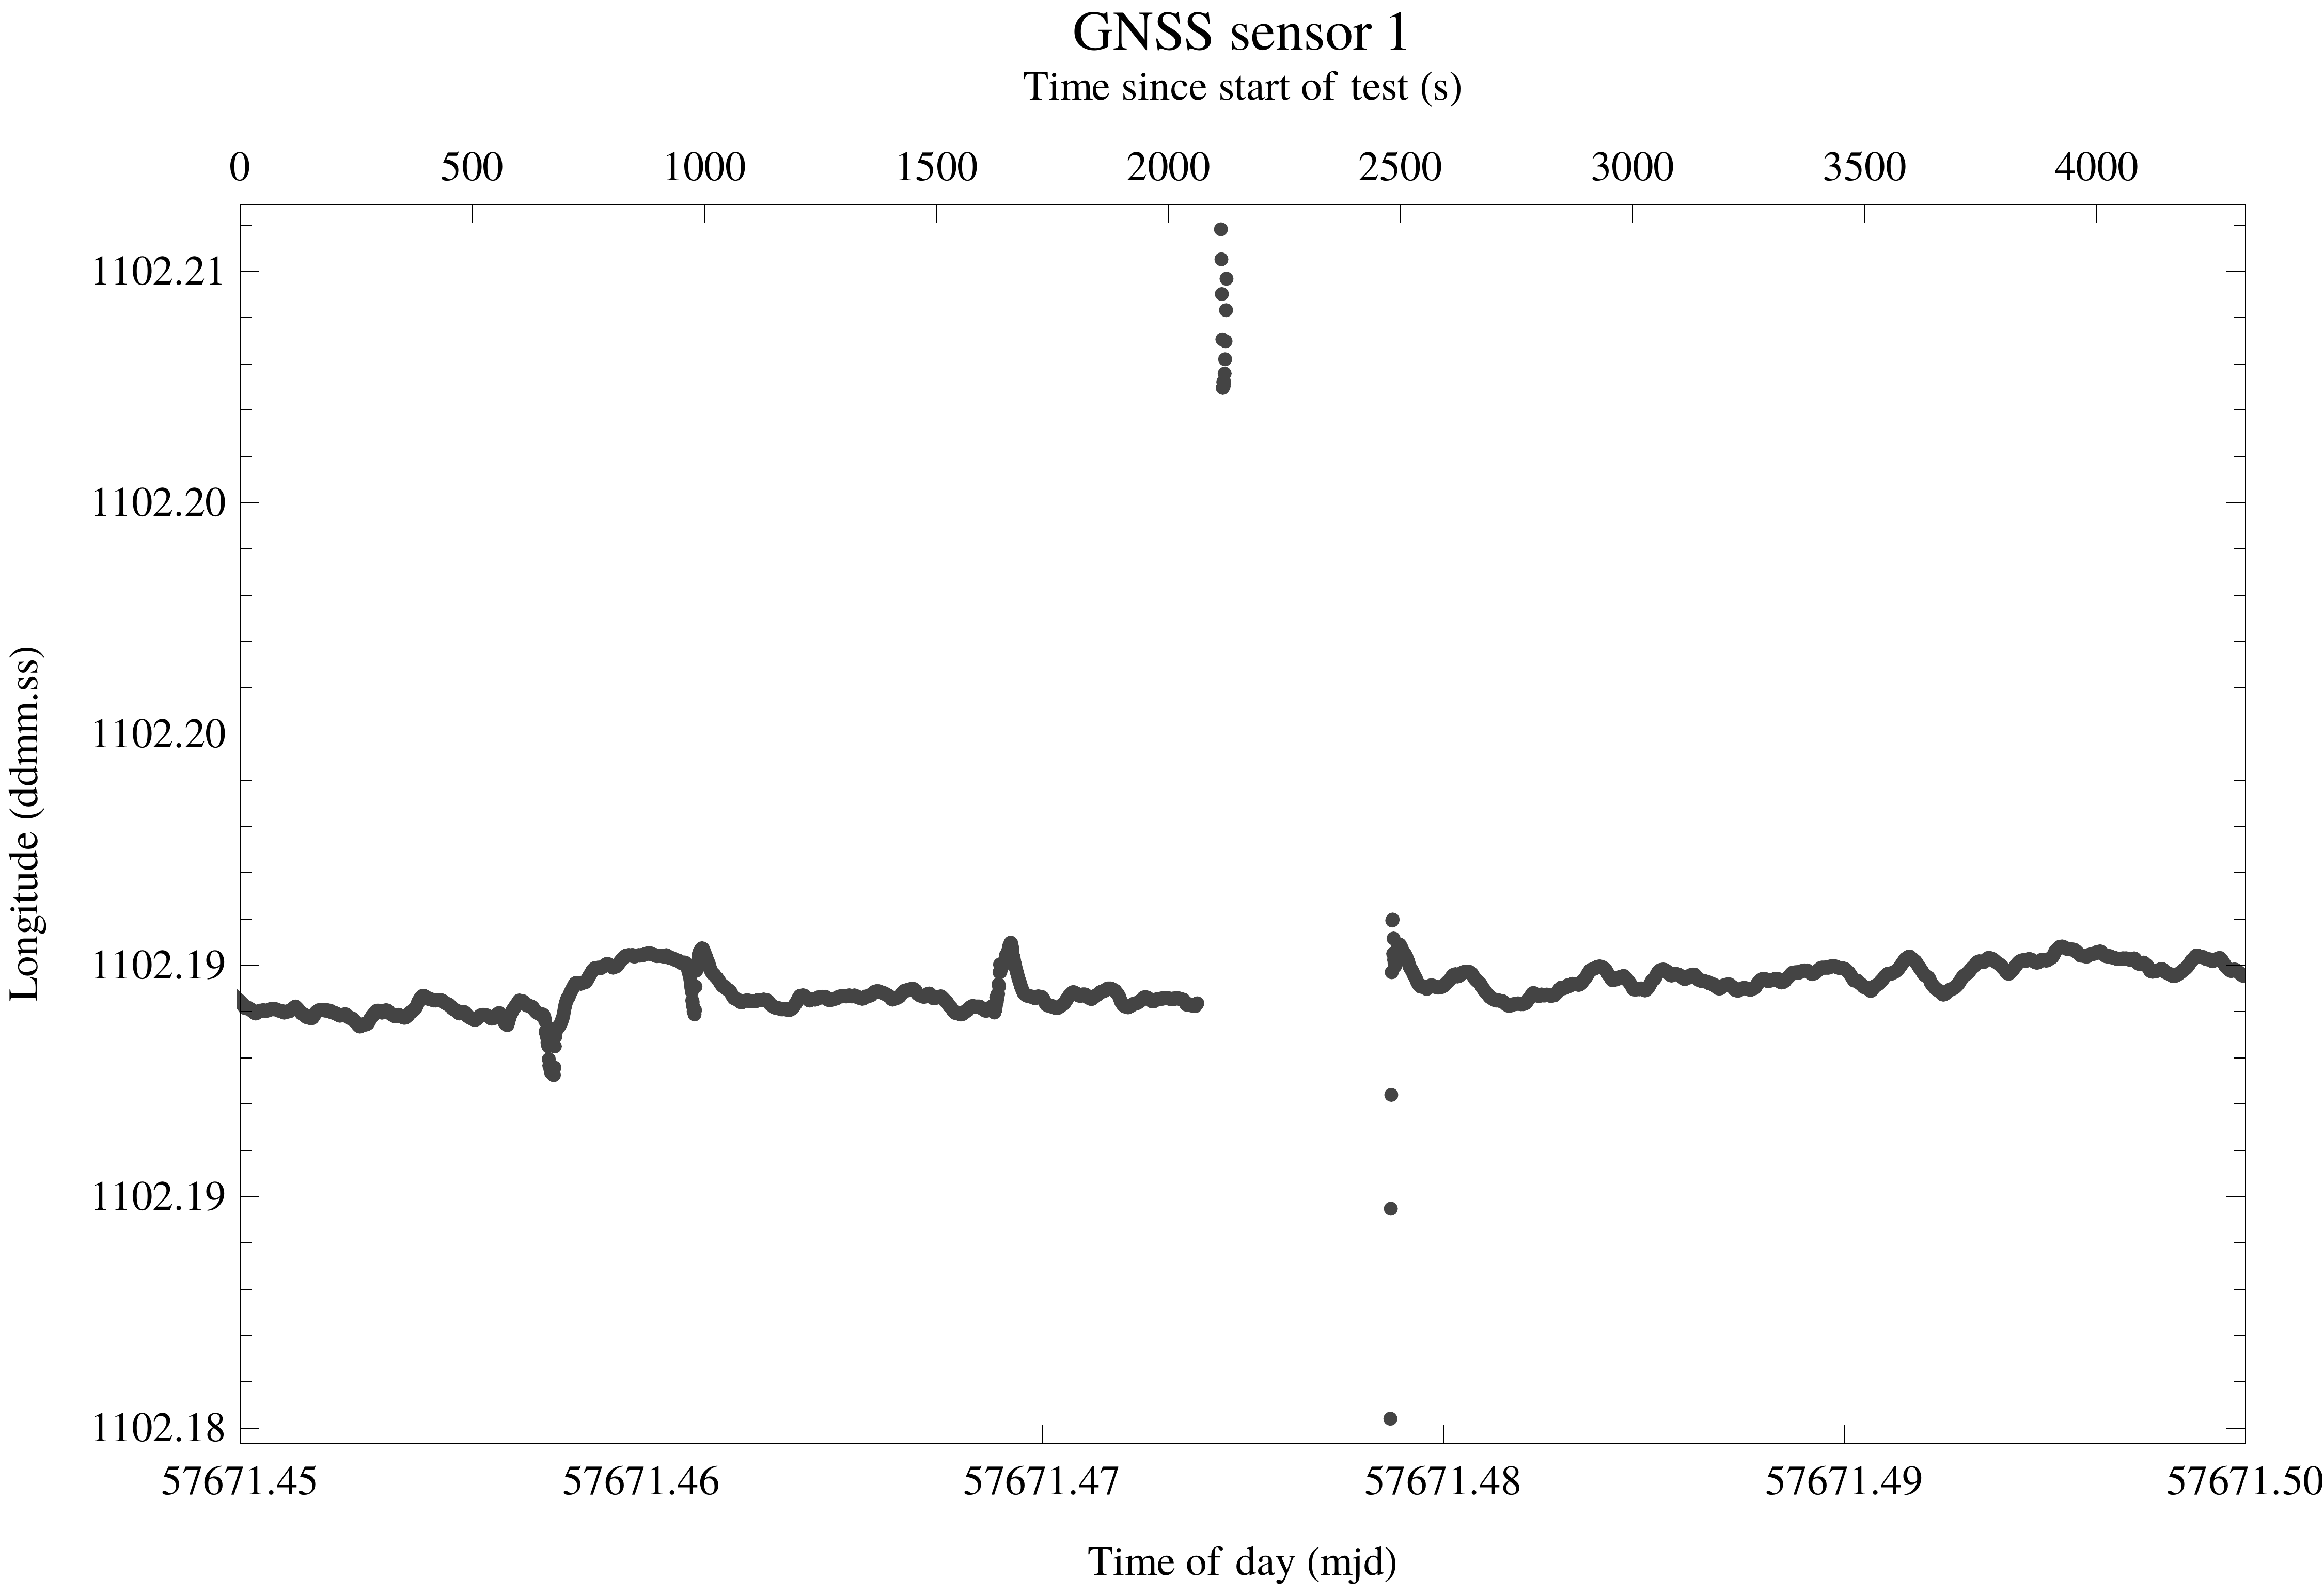
\includegraphics[width=1\textwidth]{gnssLong1-1g.png}
  \caption{The figure shows the solved longitude of the GPS receiver connected to sensor one, during test one}
  \label{sensor1_long}
\end{sidewaysfigure}
 

\begin{sidewaysfigure}
  \centering
  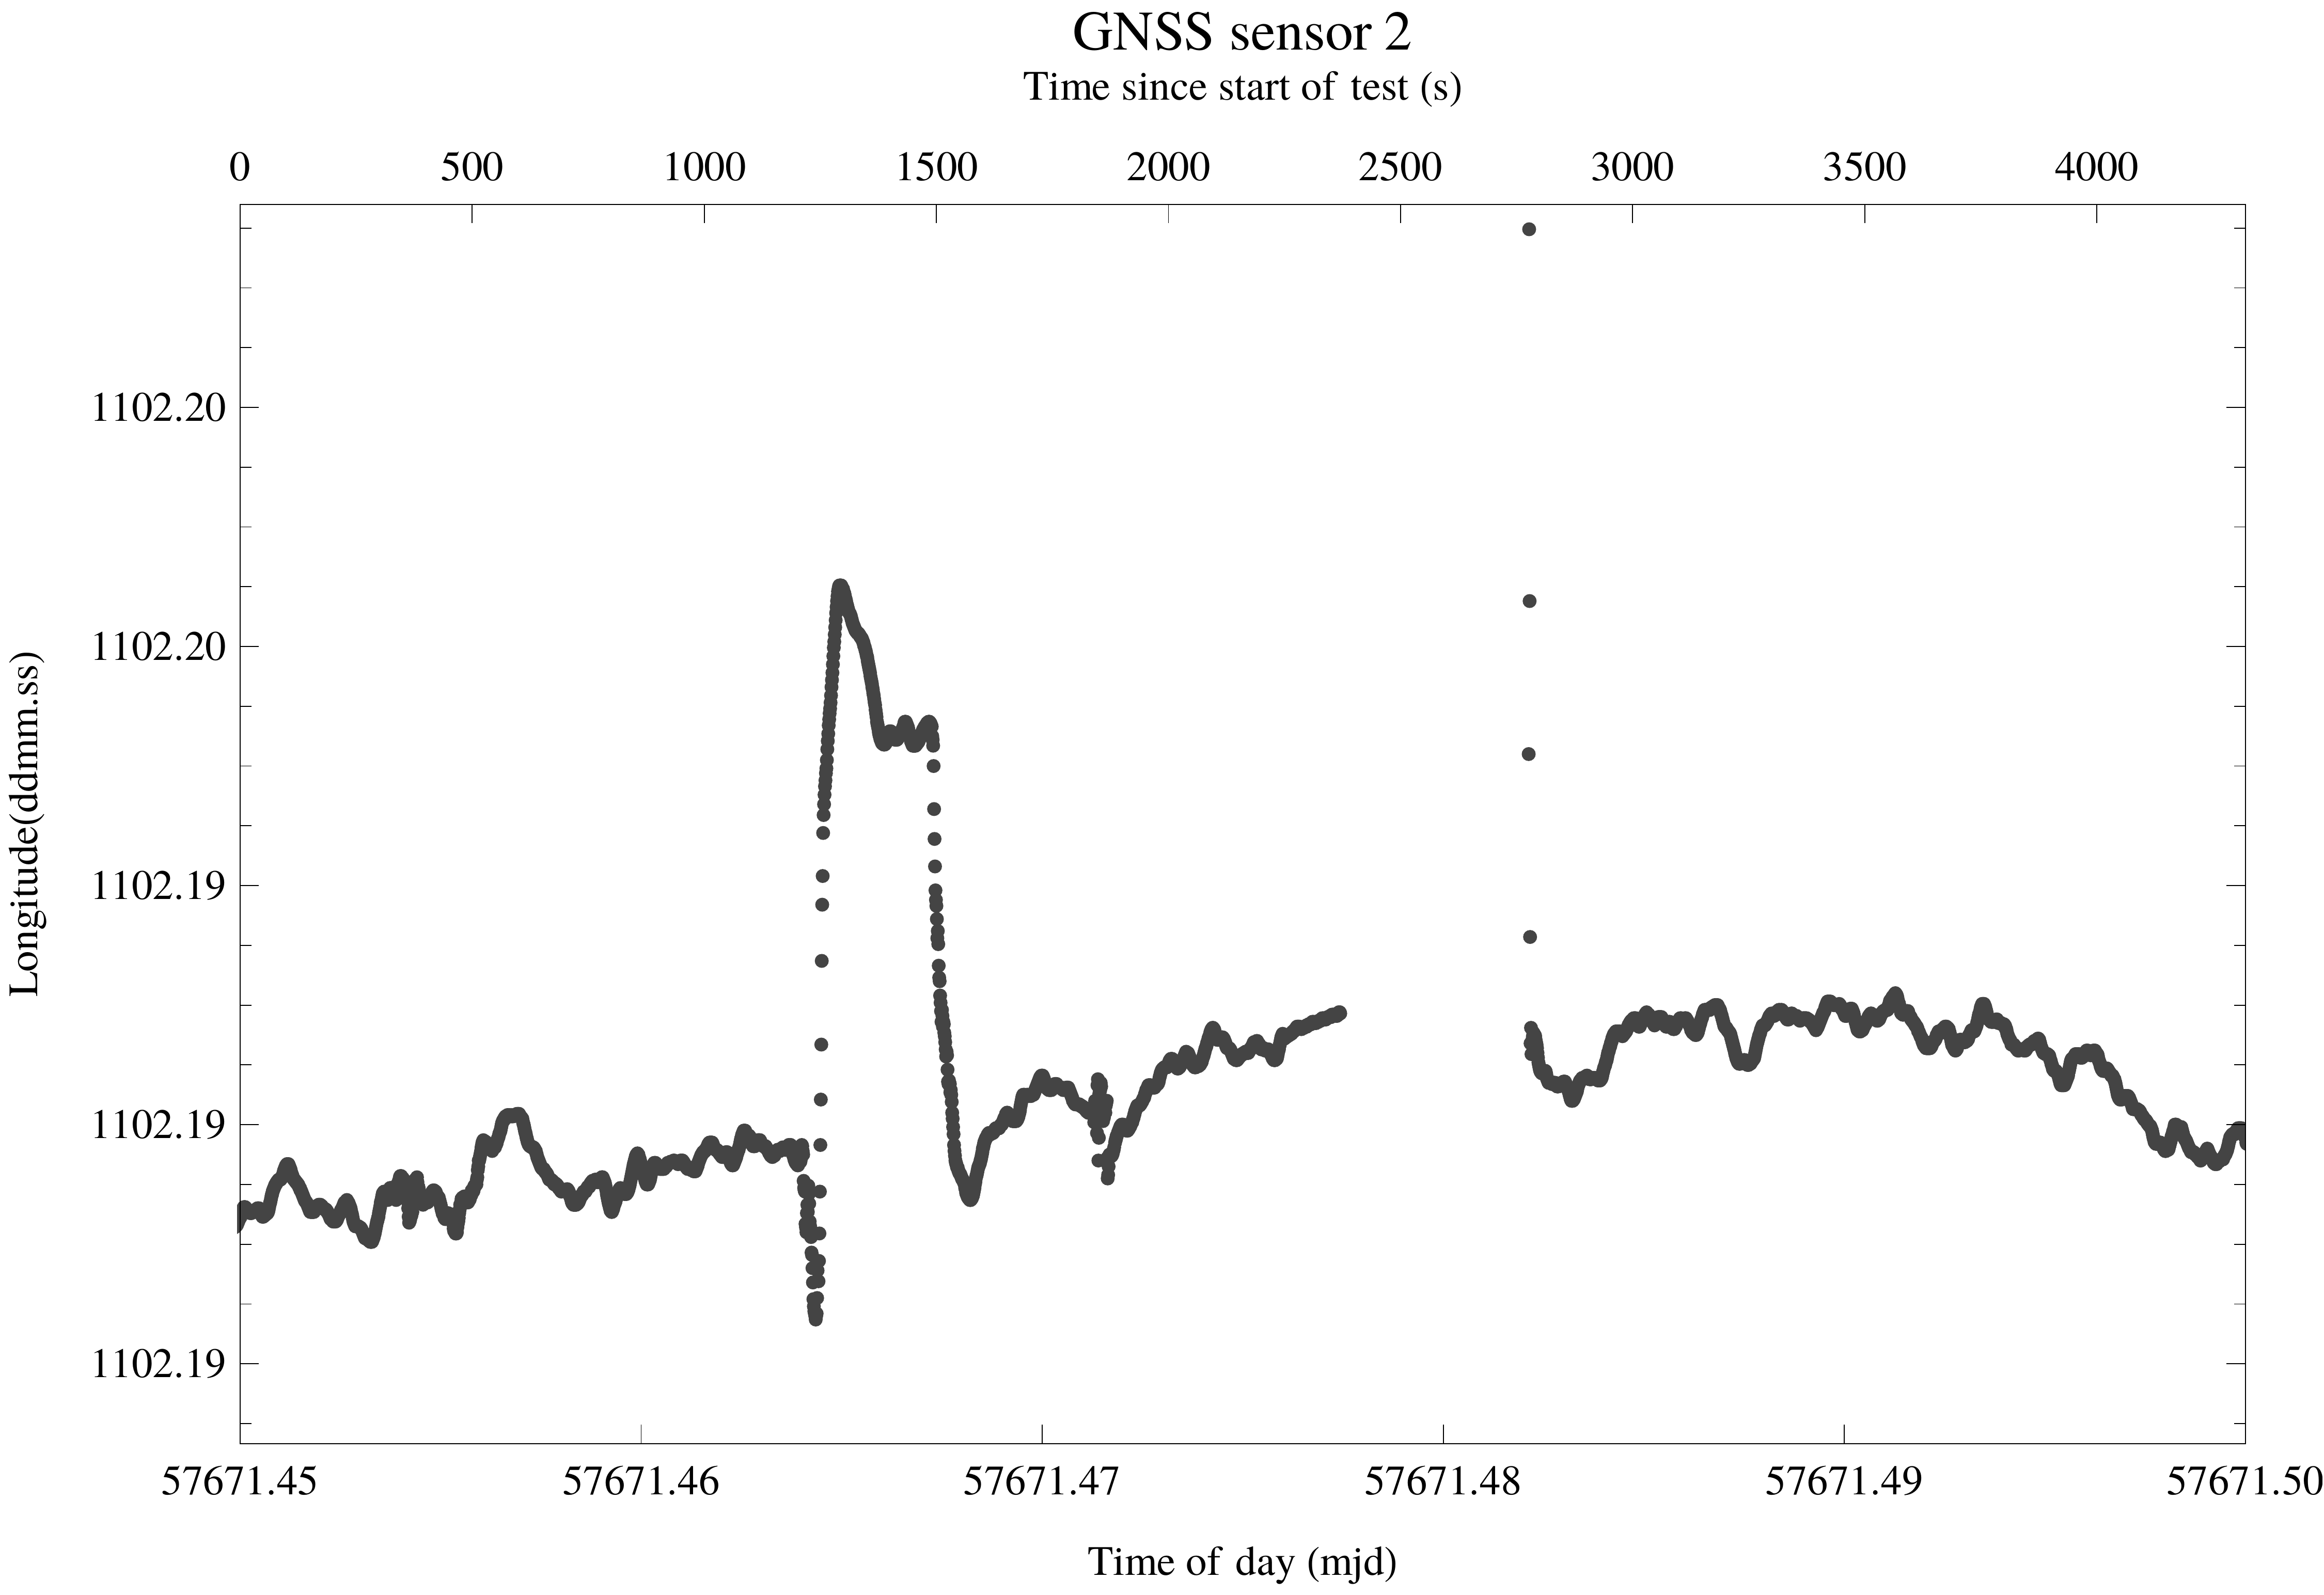
\includegraphics[width=1\textwidth]{gnssLong2-1g.png}
  \caption{The figure shows the solved longitude of the GPS receiver connected to sensor two, during test one}
  \label{sensor2_long}
\end{sidewaysfigure}
 

\begin{sidewaysfigure}
  \centering
  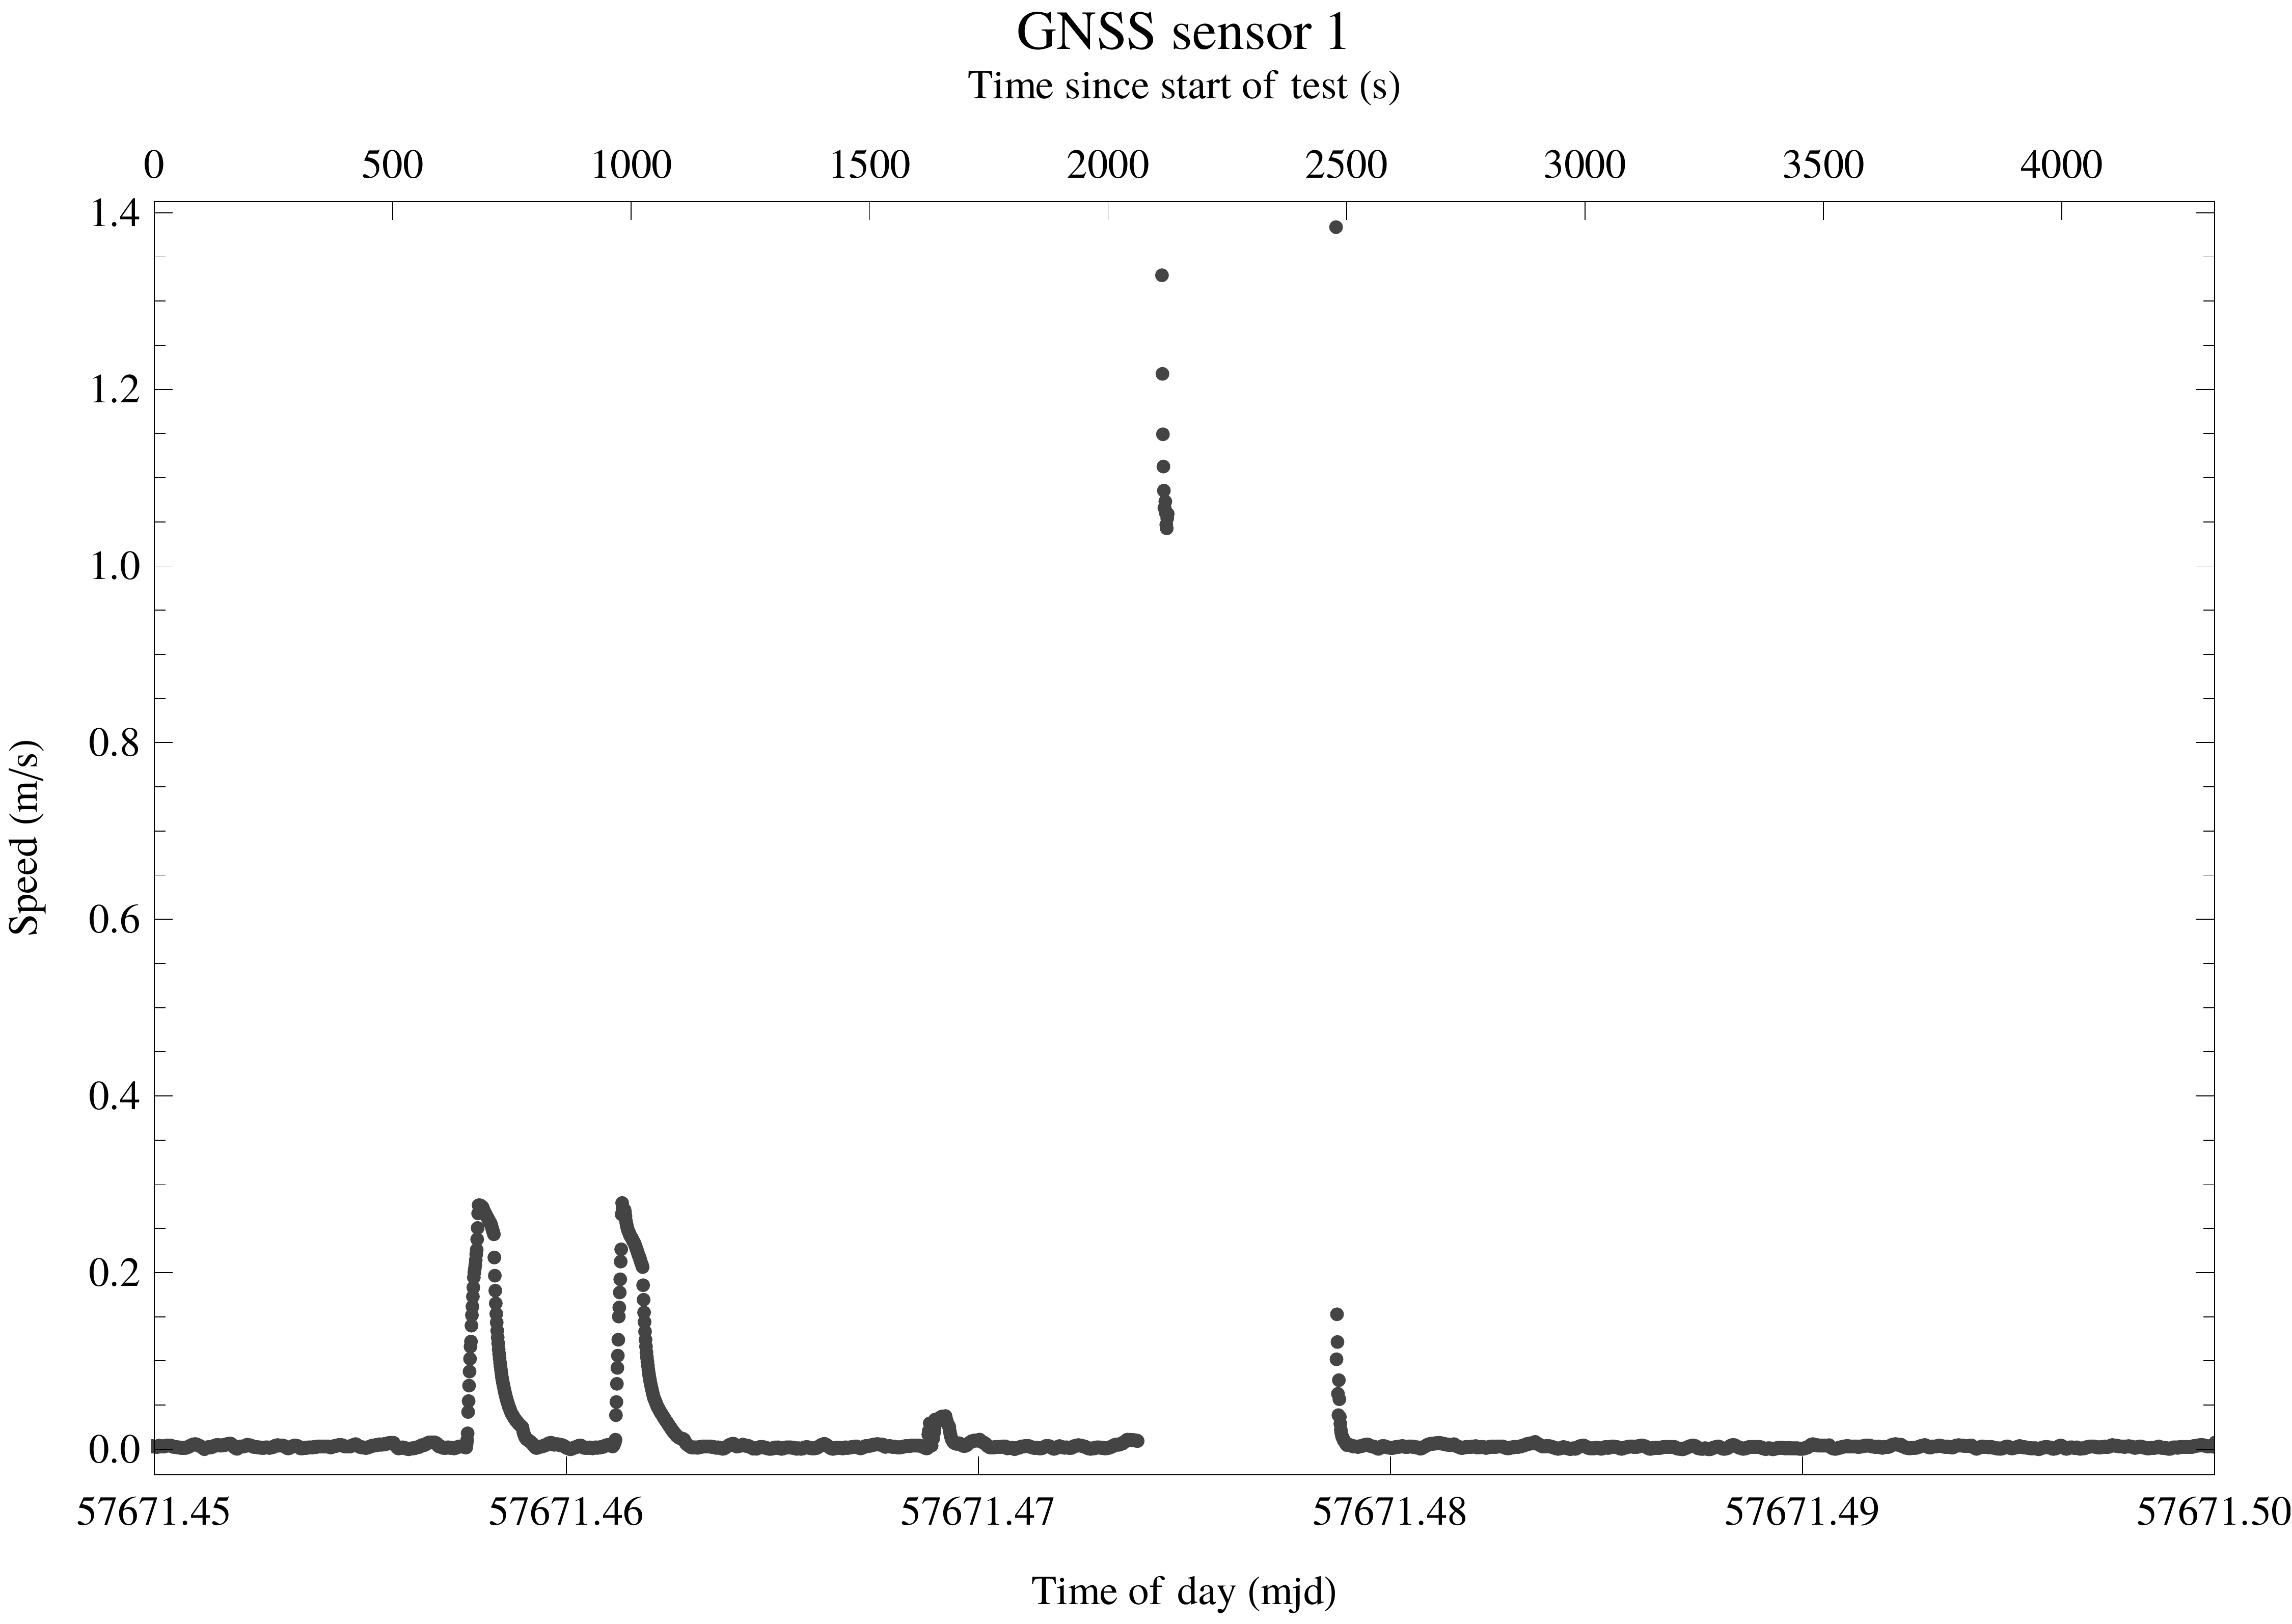
\includegraphics[width=1\textwidth]{gnssSpeed1-1g.png}
  \caption{The figure shows the solved speed of the GPS receiver connected to sensor one, during test one}
  \label{sensor1_speed}
\end{sidewaysfigure}
 

\begin{sidewaysfigure}
  \centering
  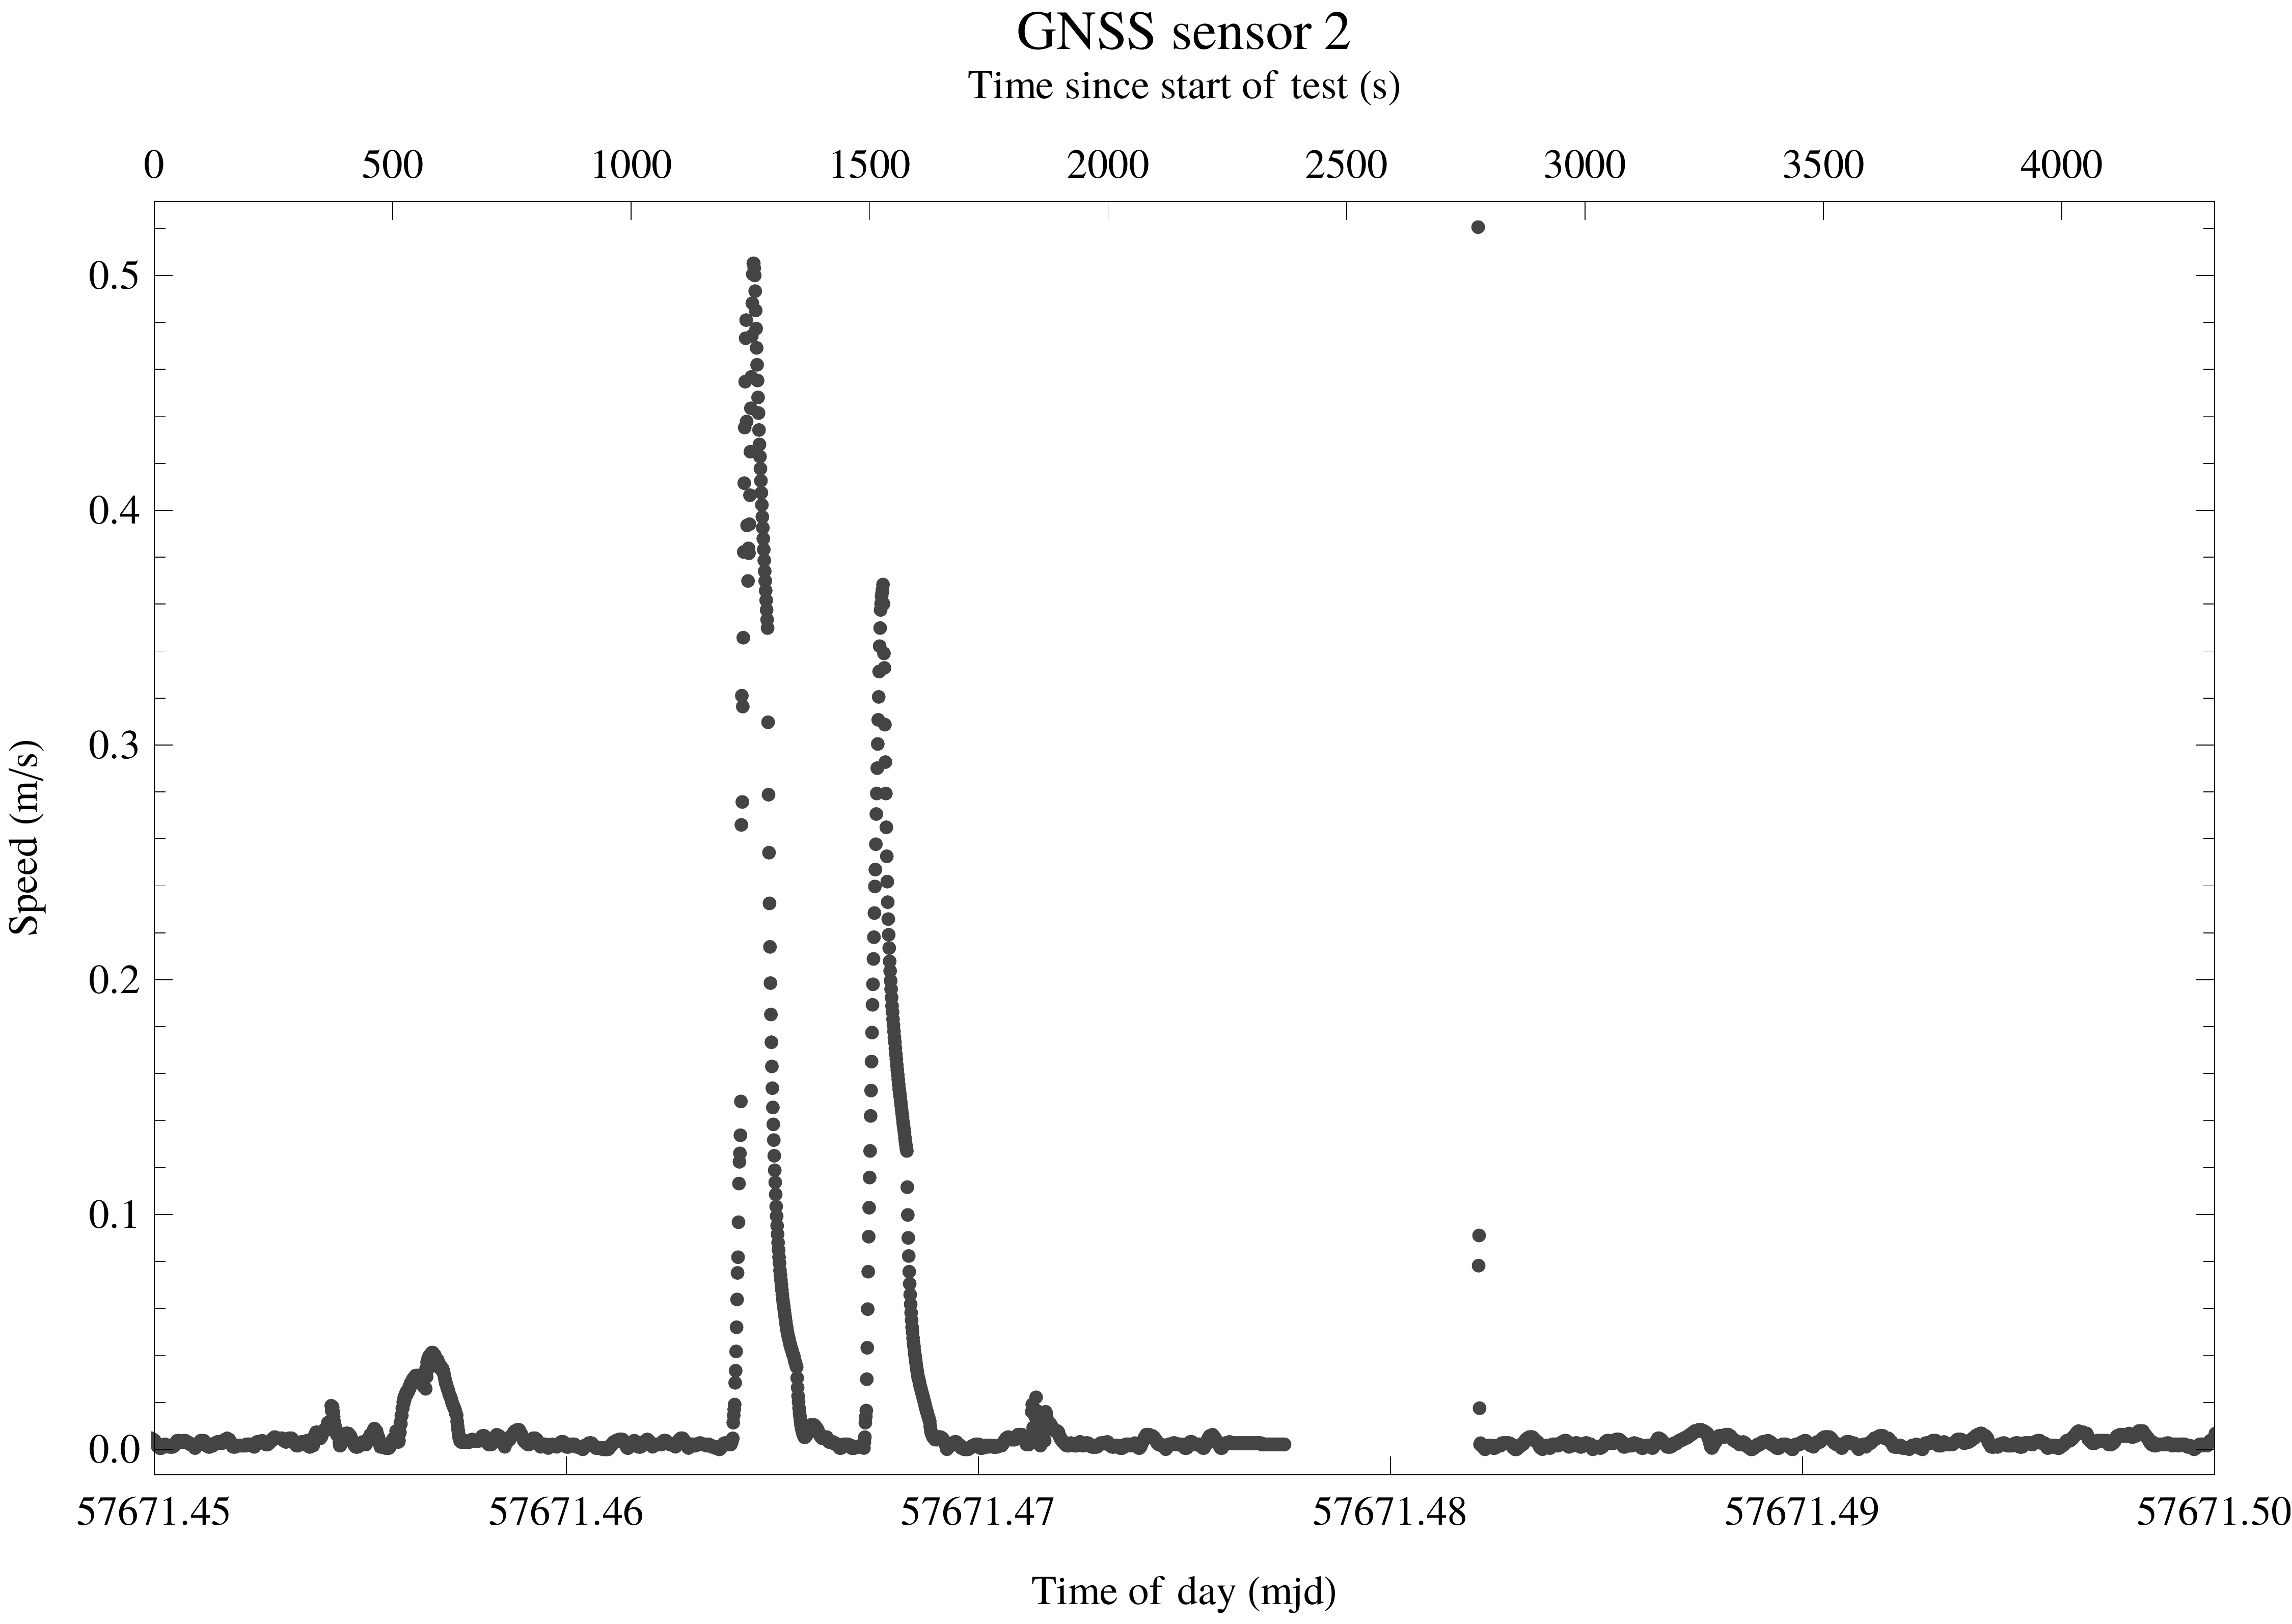
\includegraphics[width=1\textwidth]{gnssSpeed2-1g.png}
  \caption{The figure shows the solved speed of the GPS receiver connected to sensor two, during test one}
  \label{sensor2_speed}
\end{sidewaysfigure}
 

\newpage
\subsection{Timing measurements}\label{test1_measurements}
Figure \ref{cns91_tel_freq} shows the relative frequency offset ($10^{12}$) for the atomic clock. The thick dark plot in the middle is from telemetry data gathered from the atomic clock. Figure \ref{cns91_tel_phase} shows the phase offset in nanoseconds for the atomic clock. The interesting thing to observe in both of these figures, is the jump in frequency and phase offset once the antenna was covered in aluminium foil. There is also a clear correlation between movement of the antenna and the relative frequency offset as seen in figure \ref{cns91_tel_freq}. 

\begin{figure}[!htb]
  \centering
  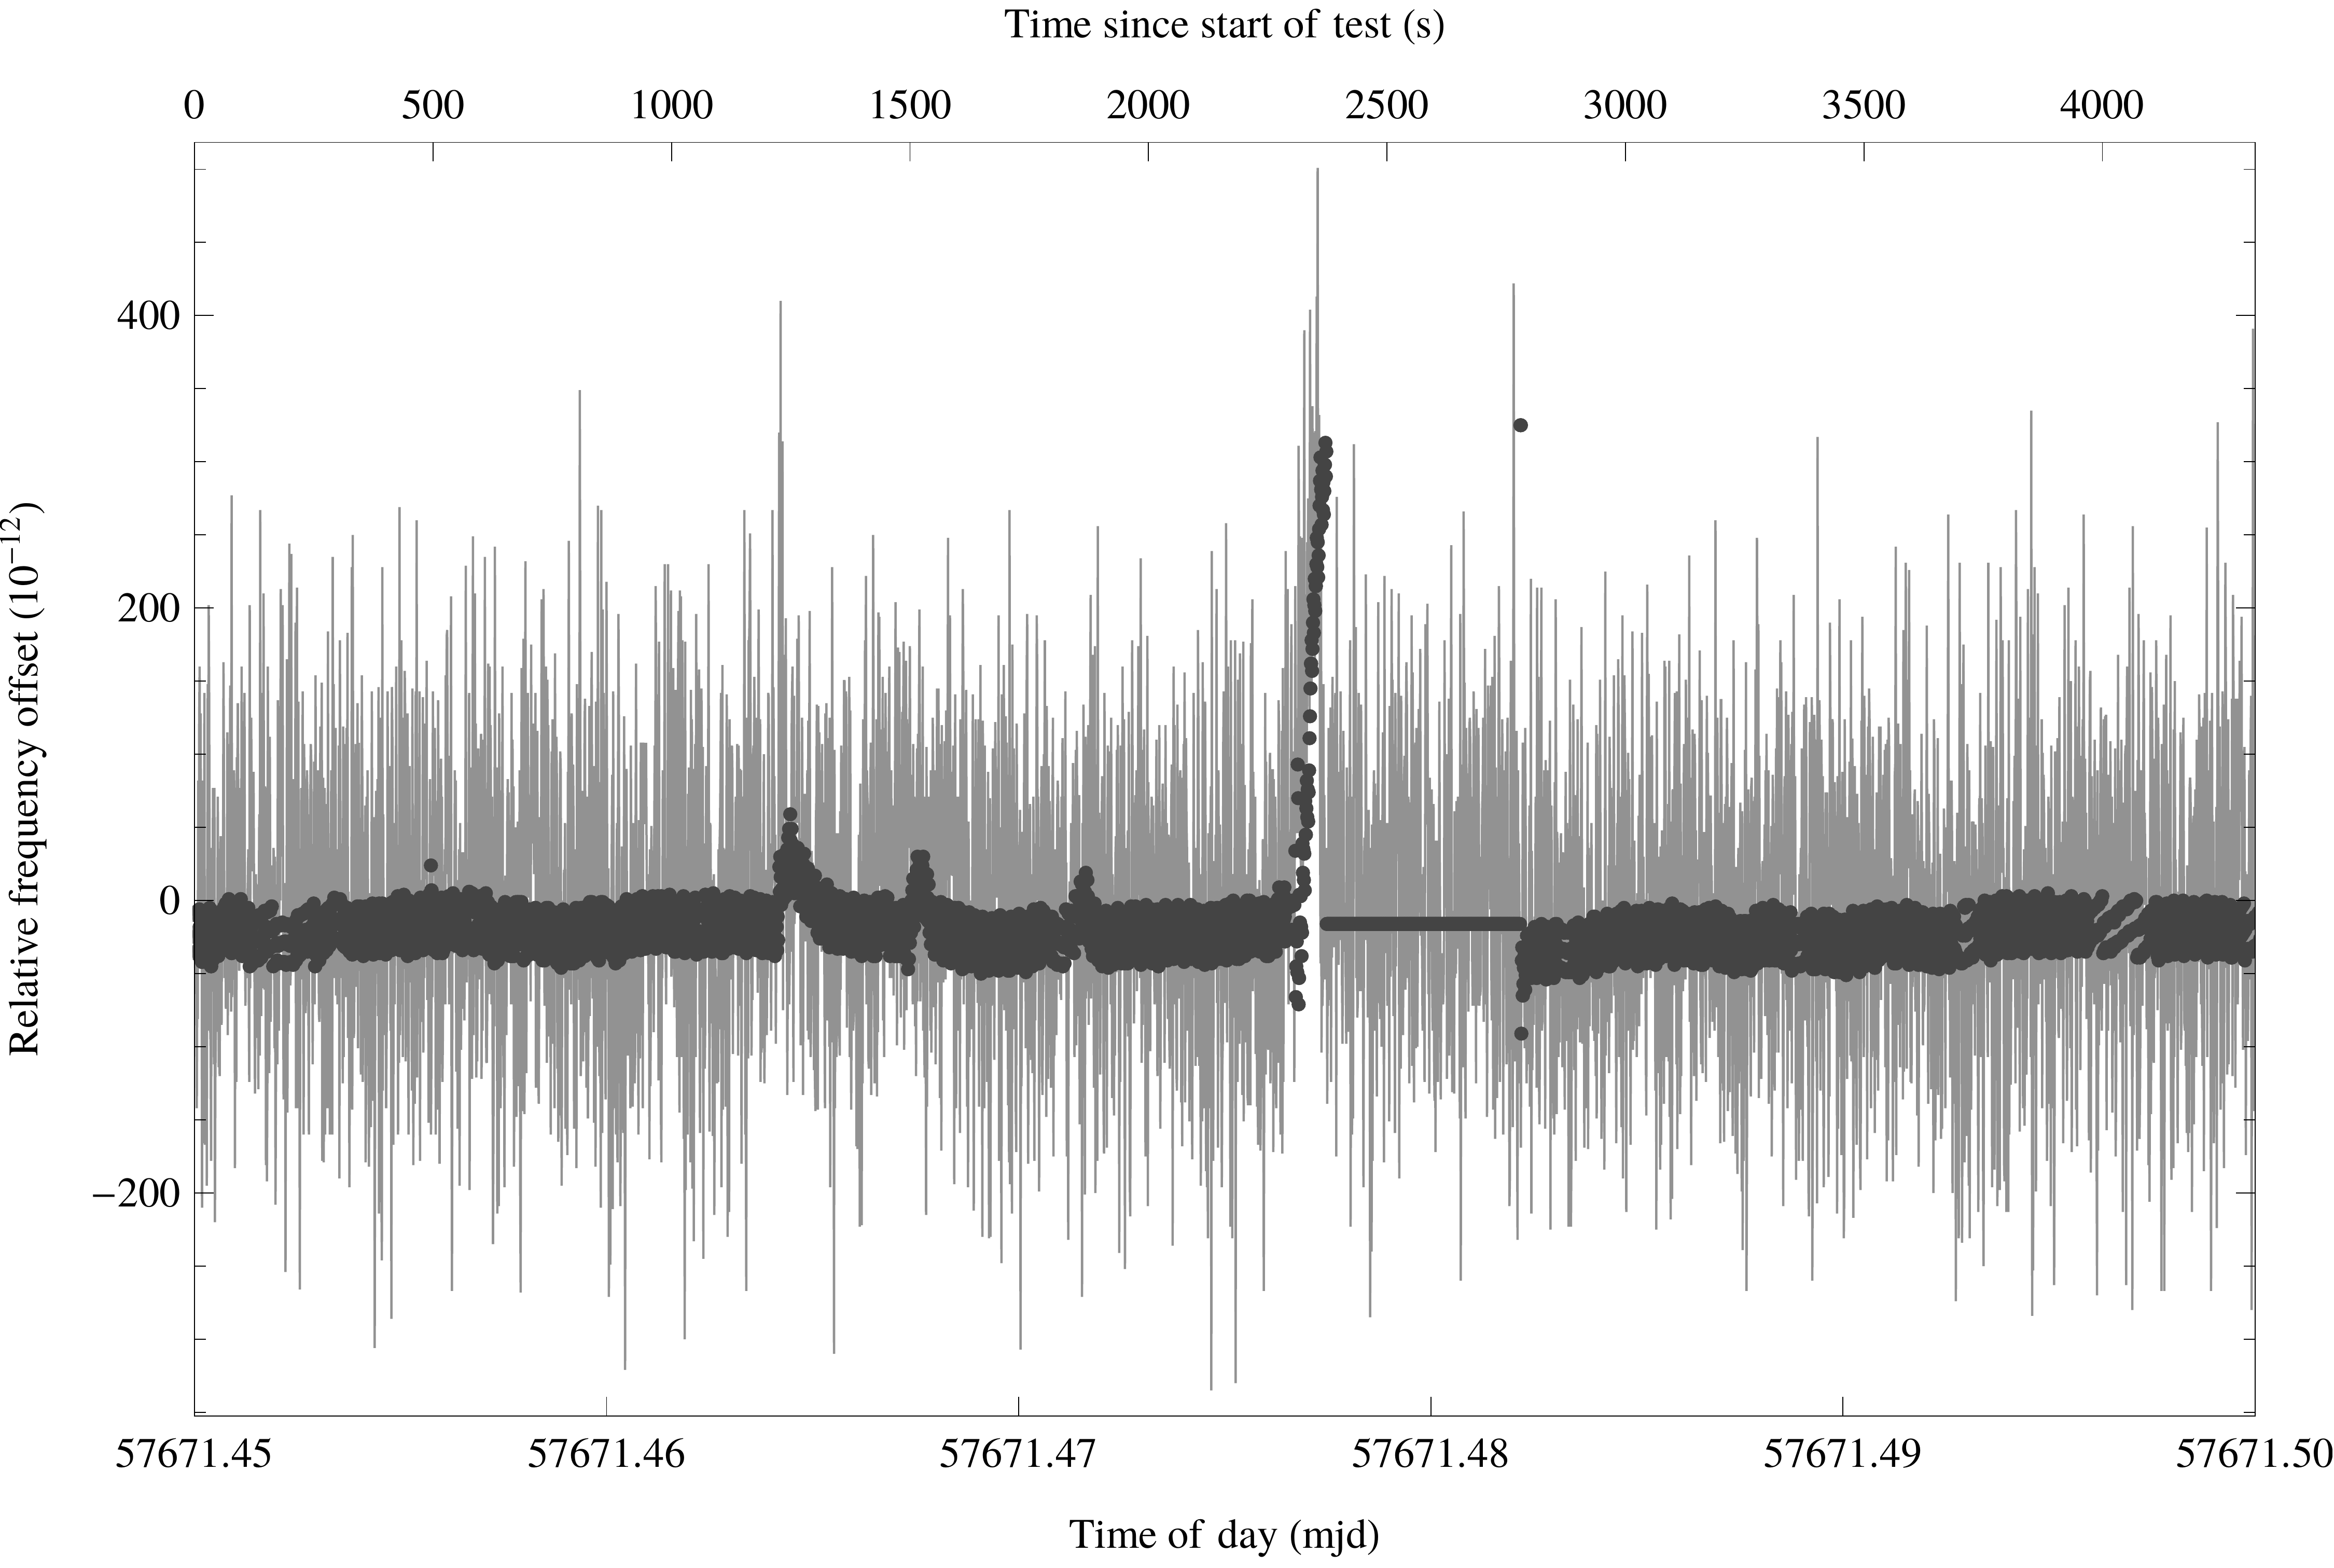
\includegraphics[width=1\textwidth]{cns91-and-csac-telemetry-frequency-1g.png}
  \caption{The figure shows the relative frequency offset for the atomic clock. The thick dark plot in the middle is from telemetry data gathered from the atomic clock. The lighter plot in the background is data from the CNT-91 frequency counter.}
  \label{cns91_tel_freq}
\end{figure} 

\begin{sidewaysfigure}
  \centering
  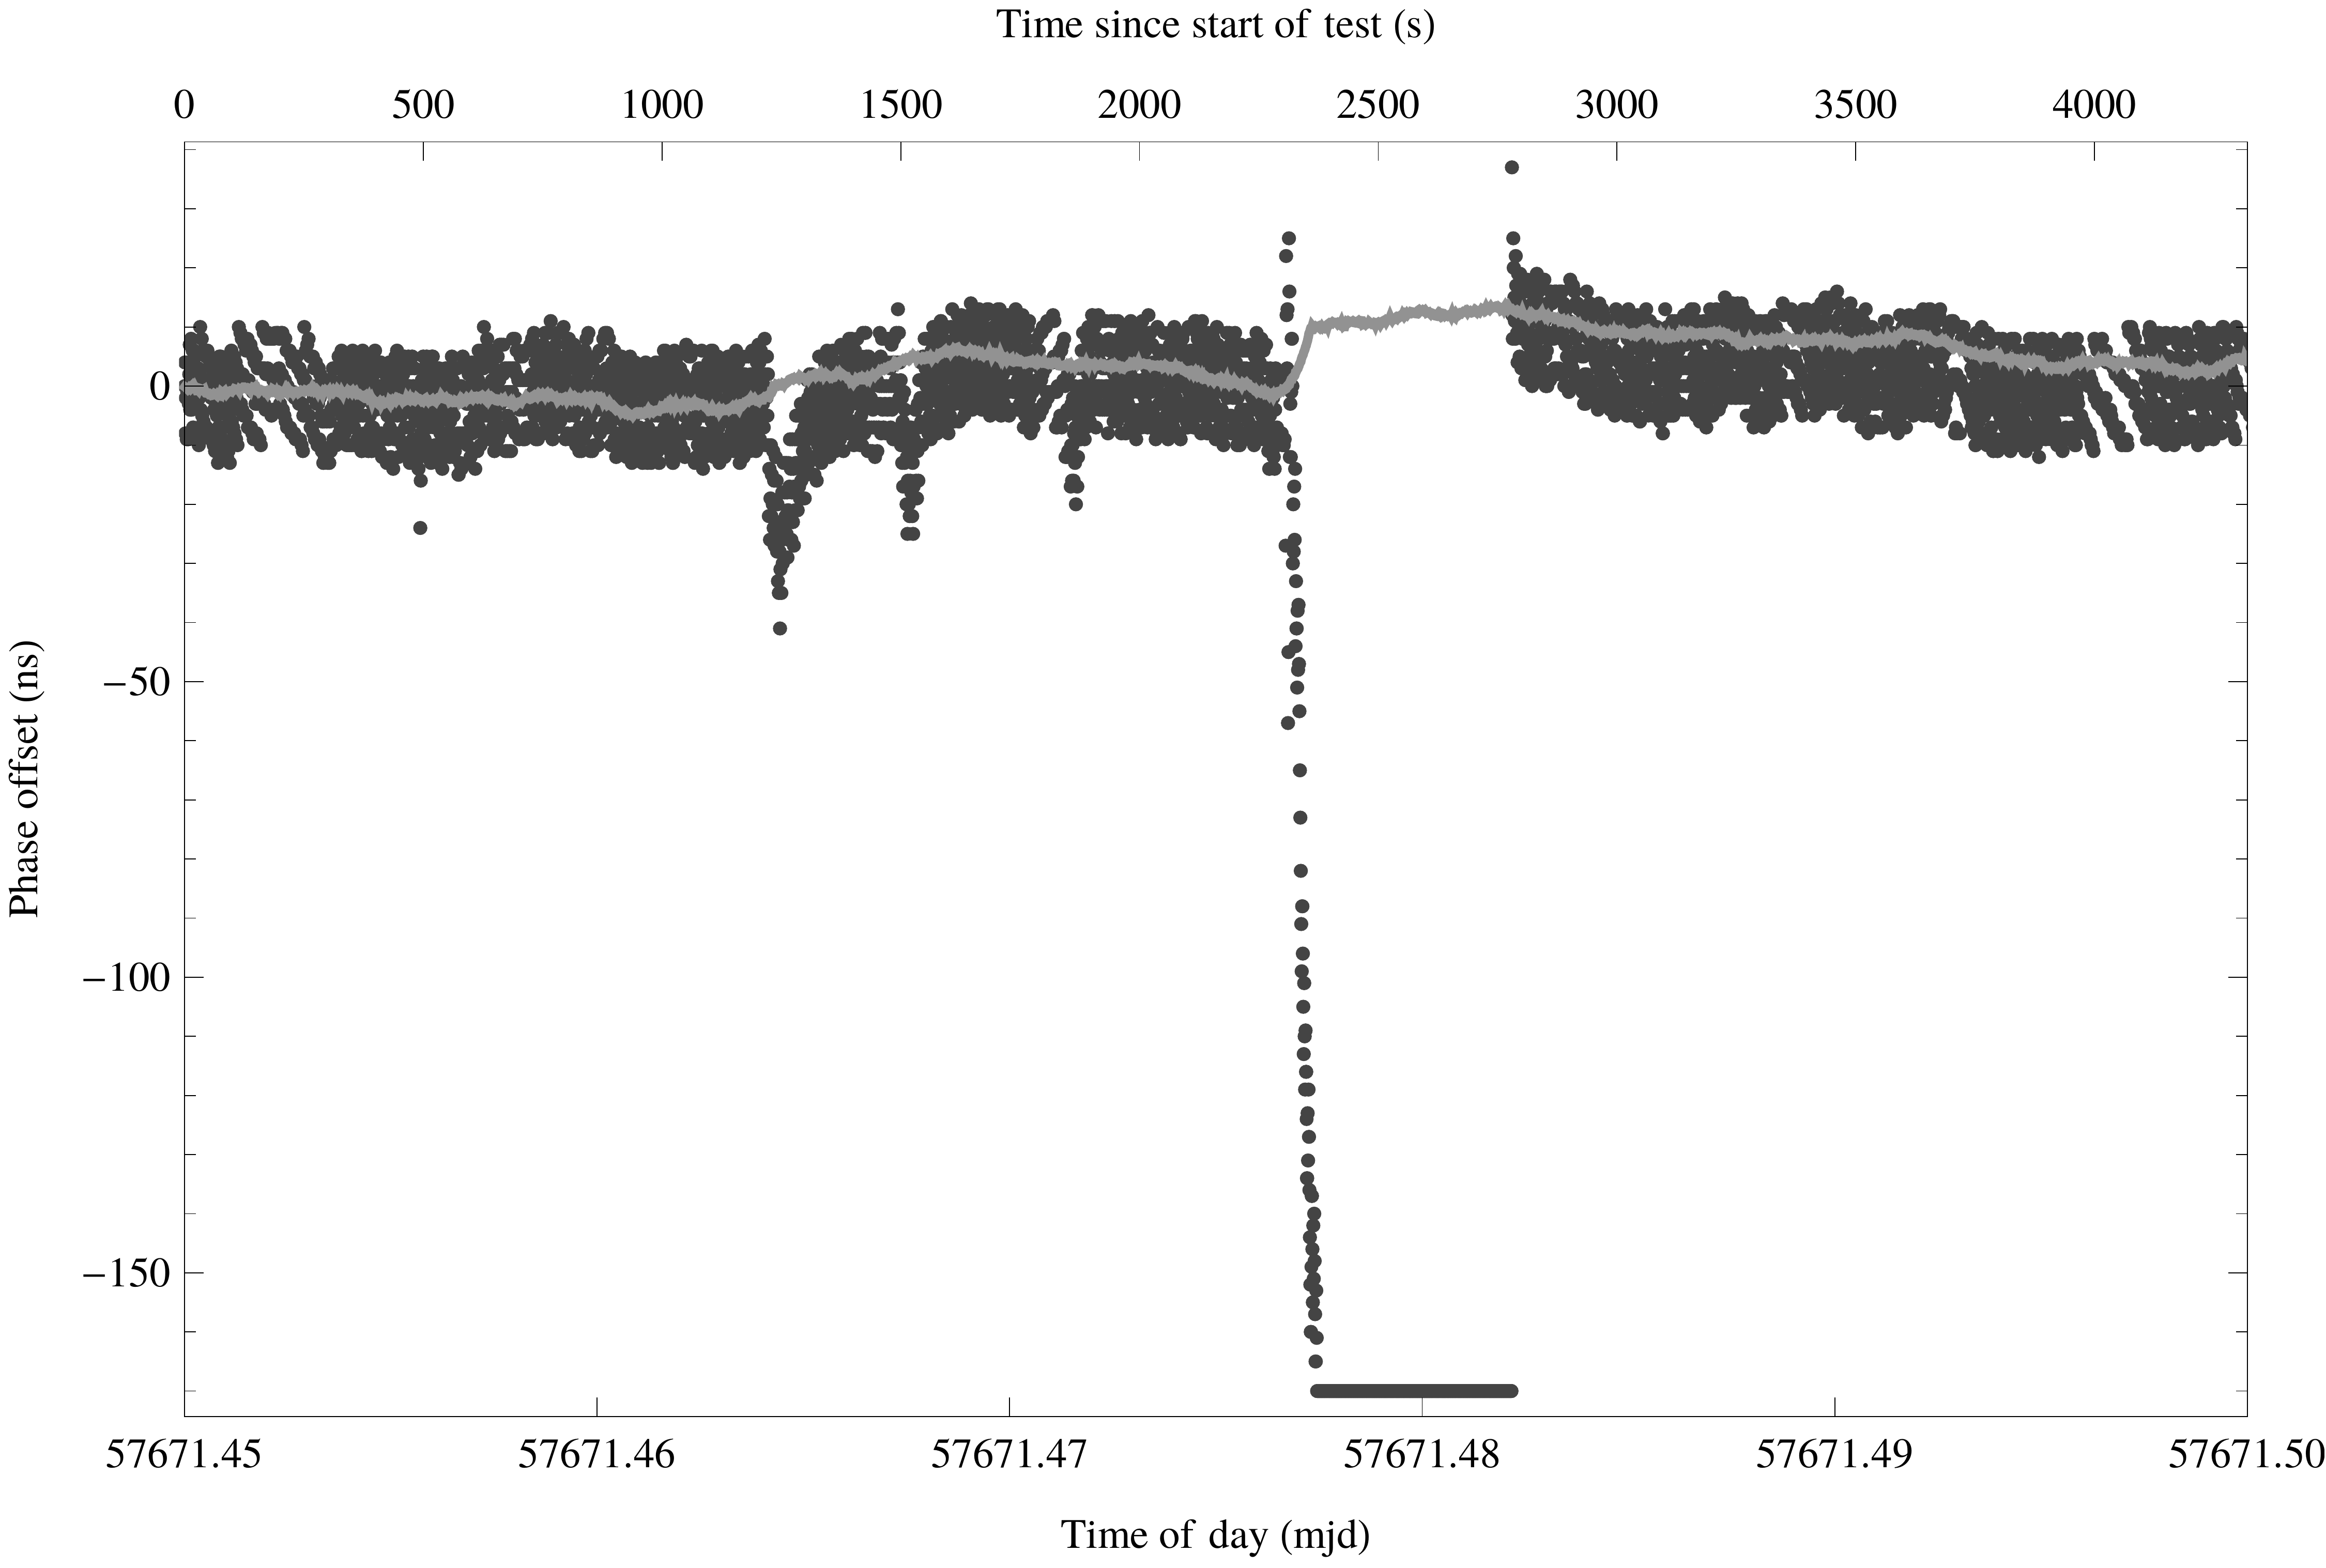
\includegraphics[width=1\textwidth]{cns91-and-csac-telemetry-phase-1g.png}
  \caption{The figure shows the phase offset in nanoseconds for the atomic clock. The thick dark plot is from telemetry data gathered from the atomic clock. The lighter thin plot is data from the CNT-91 frequency counter.}
  \label{cns91_tel_phase}
\end{sidewaysfigure}

\newpage
\subsection{Test one results}
The observations from test one revealed some surprising results. When the antennas were moved horizontally the altitude solved by sensor two dramatically changed. The movement also resulted in a change in the timing solution. The GPS filter did, however, perform as expected. We discovered that the reason why the step five and six failed to trigger the filter, was that the limit for speed (see section \ref{gps_filter_table} for more) was erroneously set too high. 

\section{Test two}\label{test2}
\subsection{Goal of test two}
The goal of the second test was to test the clock model based filters. The test should make the atomic clock controller disable the atomic clock's disciplining mode and steer the atomic clock based on the clock model's predictions. We also wanted to test the location and speed filter again to make sure we had fixed the error in the filter configuration from the last test.

\subsection{Change in setup}
The setup in test one is quite similar to test two. There is however some changes. Sensor one is no longer connected to the atomic clock controller because the location and speed filter no longer was the main priority to test. 

\subsection{Test two filter limits}
Table \ref{gps_filter_table2} shows the filter limits used in test two. Note that the speed deviation is set to 1 knot. Table \ref{clock_filter_table} shows the limits for the clock model based filters.

\begin{table}[!htb]
\centering
\caption{Filter thresholds used during test two}
\label{gps_filter_table2}
  \begin{tabular}{|l|l|l|}
  \hline
\multicolumn{1}{|c|}{Config value} & \multicolumn{1}{c|}{Sensor 2} \\ \hline
Altitude reference                 & 122.427                       \\ \hline
Longitude reference                & 1102.1934                     \\ \hline
Latitude reference                 & 5958.5231                     \\ \hline
Speed reference                    & 0                             \\ \hline
Altitude deviation                 & 10                            \\ \hline
Longitude deviation                & 0.005                         \\ \hline
Latitude deviation                 & 0.005                         \\ \hline
Speed deviation                    & 1                             \\ \hline
\end{tabular}
\end{table}

\begin{table}[!htb]
\centering
\caption{Clock model filter configuration}
\label{clock_filter_table}
\begin{tabular}{|l|l|}
\hline
Phase limit      & 50     \\ \hline
Steer limit      & 50 \\ \hline
Time constant    & 10000 \\ \hline
Warmup time      & 2         \\ \hline
Prediction limit & 200        \\ \hline
\end{tabular}
\end{table}

\newpage
\subsection{Description}\label{test2_description}
The description of test two is similar to test one (see section \ref{test1_description}). One difference is that greater care was taken in obtaining an accurate time for the steps.

\begin{itemize}
  \item\relax 13:12:00 - 125: Started to move antenna two towards north.
  \item\relax 13:12:45 - 170: Reached destination.
  \item\relax 13:18:00 - 485: Started the move back to original location.
  \item\relax 13:19:00 - 545: Reached destination.
  \item\relax 13:23:00 - 785: Waved the antenna around at an increasing tempo in a half circle motion.
  \item\relax 13:23:45 - 830: Stopped waving.
  \item\relax 13:27:00 - 1070: Manually enabled the disciplining of the atomic clock.
\end{itemize}

\subsection{Observations}\label{test2_observations}
\subsubsection{Sensor Server logs}
By reviewing the log produced by the sensor server the following was observed:

\begin{itemize}
  \item No false positives, the filters were not triggered before the test started.
  \item The location and speed filter was triggered by at 13:12:10 and cleared at 13:19:54
  \begin{lstlisting}
    [10/24/16 - 13:12:10] [ ALARM ] Sensor 2 triggered LS filter!
    ...
    [10/24/16 - 13:19:54] [ ALARM ] Sensor 2 cleared LS filter!
  \end{lstlisting}
  \item The location and speed filter was triggered again at 13:23:12 for only a second. It was then triggered again two seconds later and was not cleared until 13:23:43.
    \begin{lstlisting}
    [10/24/16 - 13:23:12] [ ALARM ] Sensor 2 triggered LS filter!
    ...
    [10/24/16 - 13:23:13] [ ALARM ] Sensor 2 cleared LS filter!
    ...
    [10/24/16 - 13:23:15] [ ALARM ] Sensor 2 triggered LS filter!
    ...
    [10/24/16 - 13:23:43] [ ALARM ] Sensor 2 cleared LS filter!
  \end{lstlisting}
  \item More interesting was the fact that the \textit{Frequency correction filter} was triggered.
    \begin{lstlisting}
      [10/24/16 - 13:12:42] [ ALARM ] Steer > predicted!
    \end{lstlisting}
\end{itemize}

\subsubsection{GPS data}\label{gpsdata_test2}
Figure \ref{sensor2_everything} shows the plotted GPS data collected during test two. As with the GPS data observed during test one, there is a clear correlation between the plotted data and when the antenna was moved. The strange phenomena as described in test one (\ref{gpsdata_test1}) where the altitude was reported to be way too low, occurred in test two as well. 

\begin{figure}
  \centering
  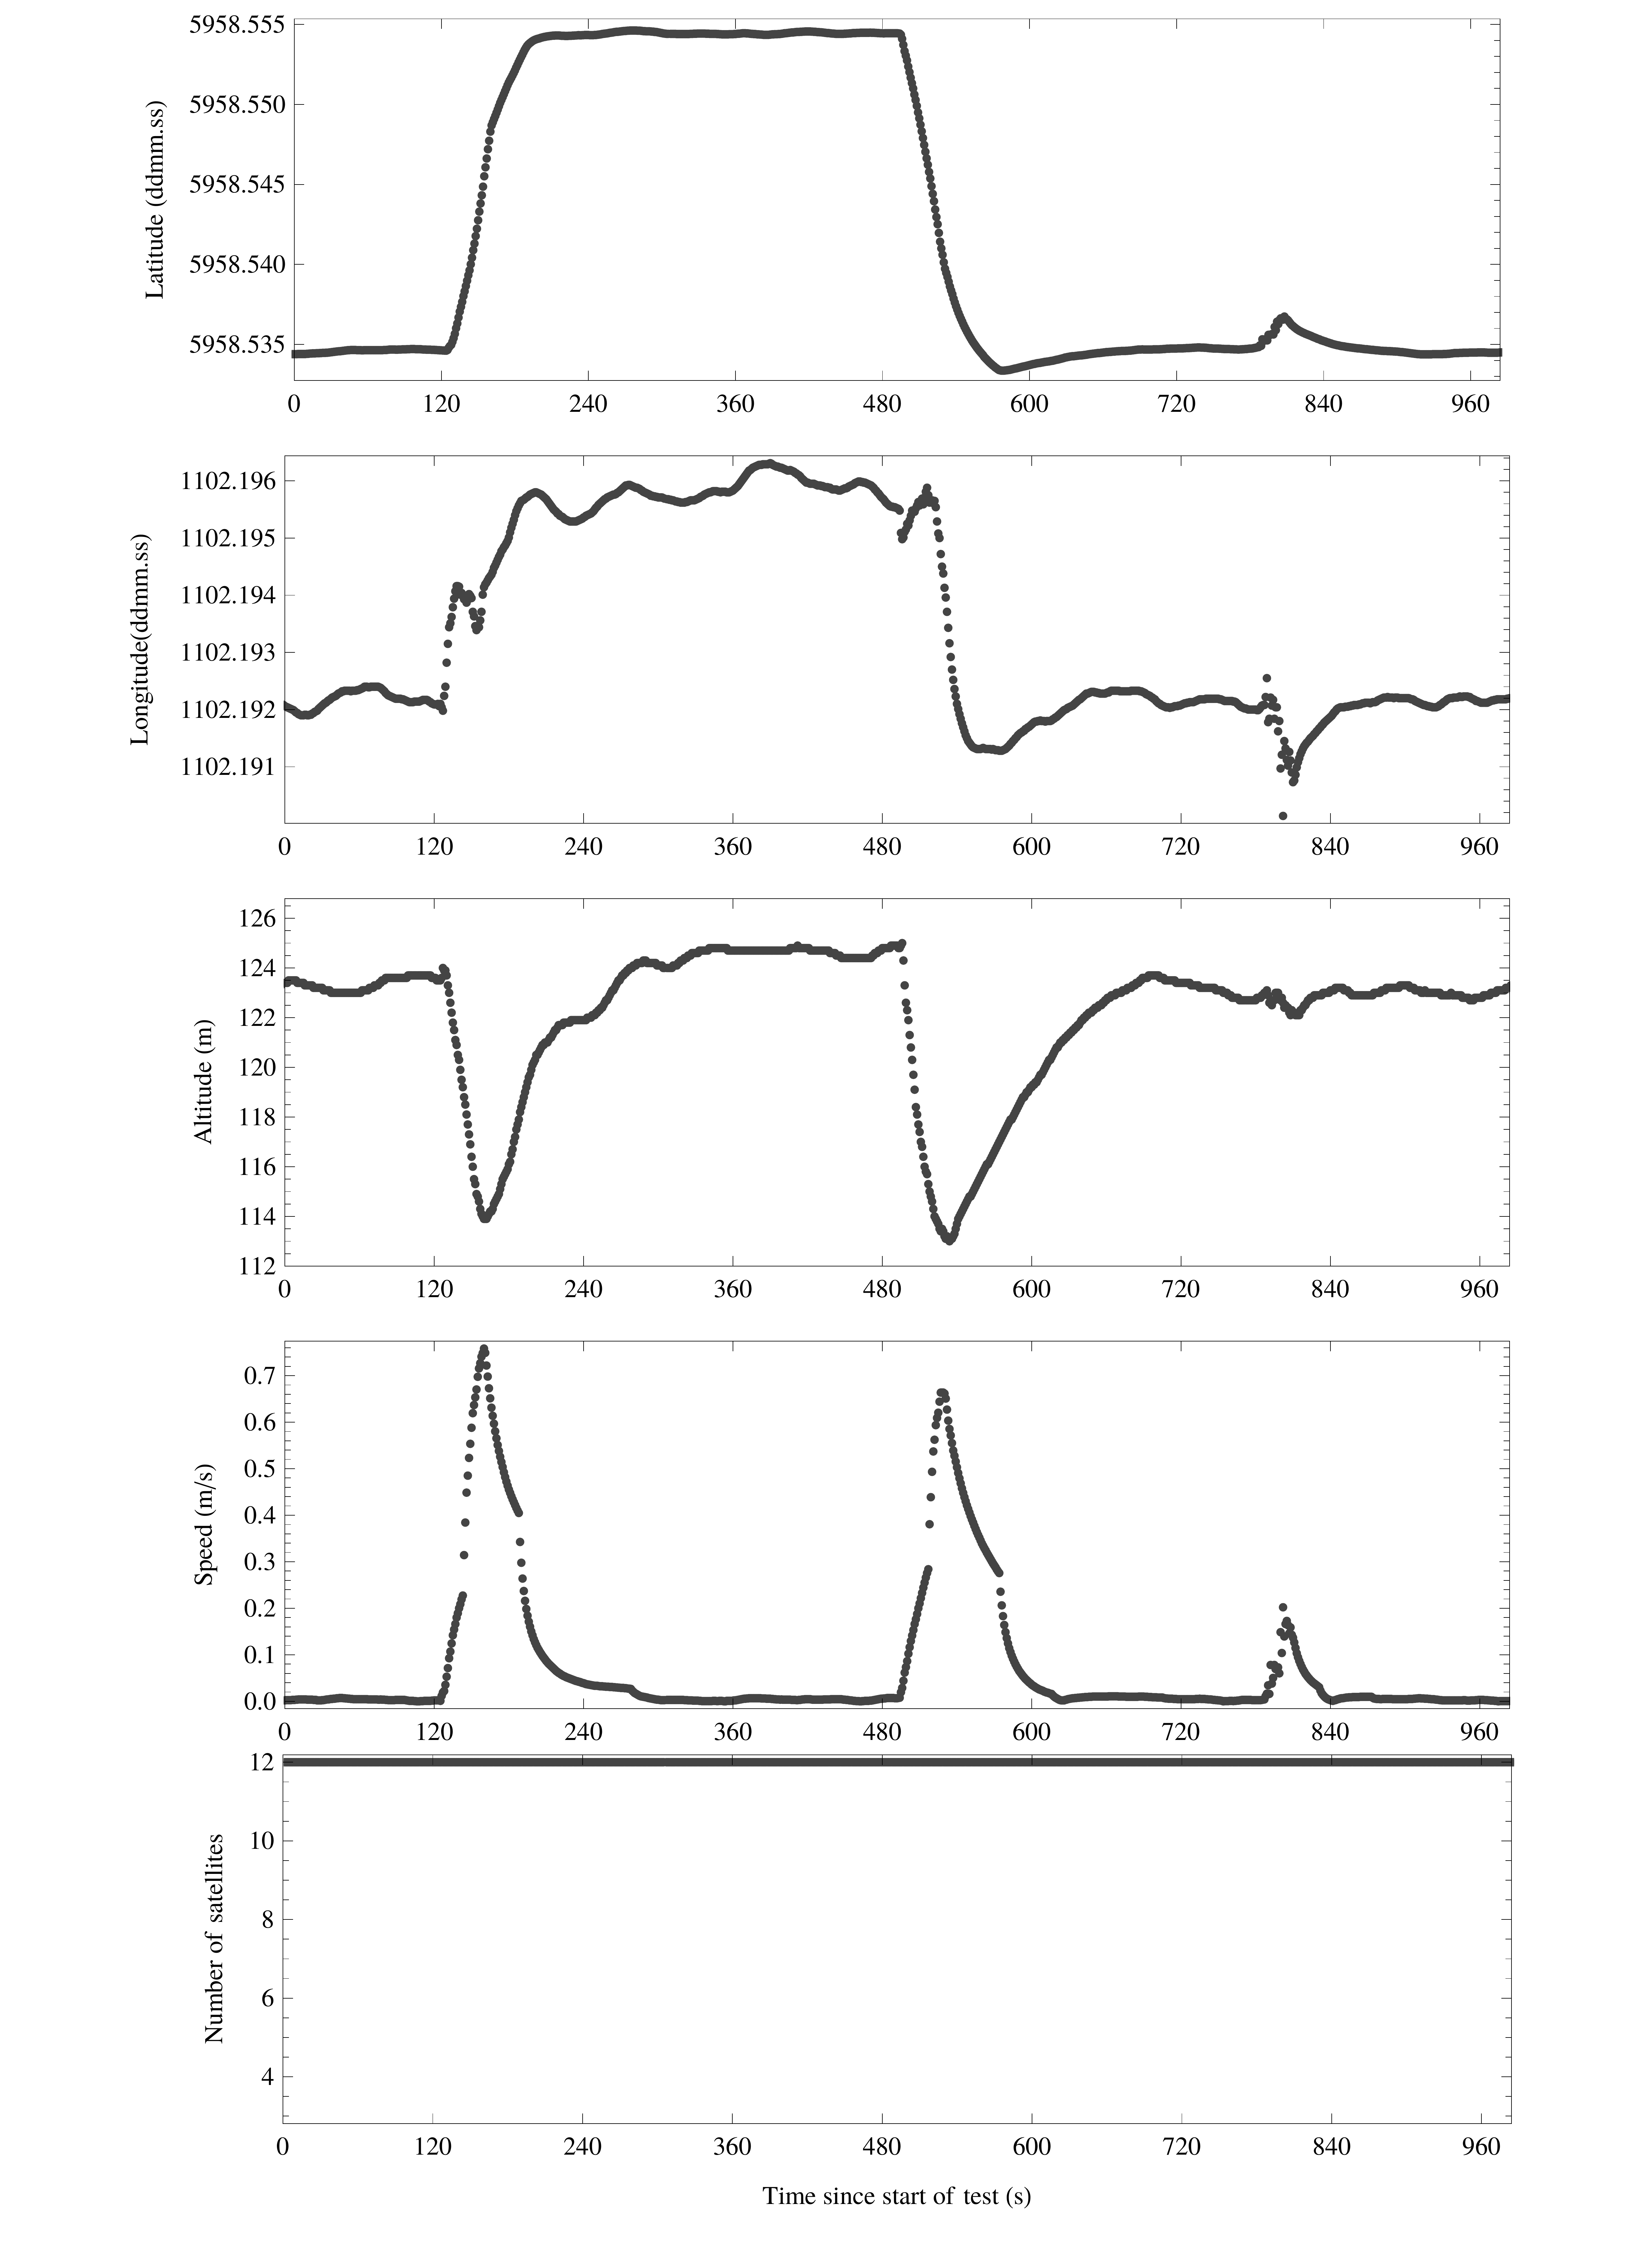
\includegraphics[width=1\textwidth]{20161024-test2-sensor2-multipanel-1g.png}
  \caption{The figure shows (from the top) the latitude, longitude, altitude, speed and number of satellites as plotted from the GPS data collected during test two.}
  \label{sensor2_everything}
\end{figure} 

\newpage
\subsection{Timing measurements}\label{test2_meaurements}
Figure \ref{sensor2_measure} shows measurements done during test two as two graphs with two time series each. The thin solid line in the top panel shows phase offset in nanoseconds. It reveals that the atomic clock was \textit{not} steered based on the clock model once the disciplining was disabled. The panel at the bottom of figure \ref{sensor2_measure} shows relative frequency offset as measured by the CNT-91 frequency counter. The thin darkly colored line is a plot of the data received as telemetry from the atomic clock. The plot shows that the disciplining of the atomic clock stopped after roughly 140 seconds. 

\subsection{Test two results}
As mentioned under subsection \ref{test2_meaurements}, the disciplining of the atomic clock was successfully deactivated when the steer value reported by the atomic clock exceeded the steer value that was predicted by the model. The phase jump filter was not triggered because the phase offset never reached the configured limit. The frequency correction filter, on the other hand, was triggered because the steer value exceeded the configured limit (see table \ref{clock_filter_table} for limits). It also shows that the atomic clock sadly was \textit{not} steered using the clock model.

\begin{figure}
  \centering
  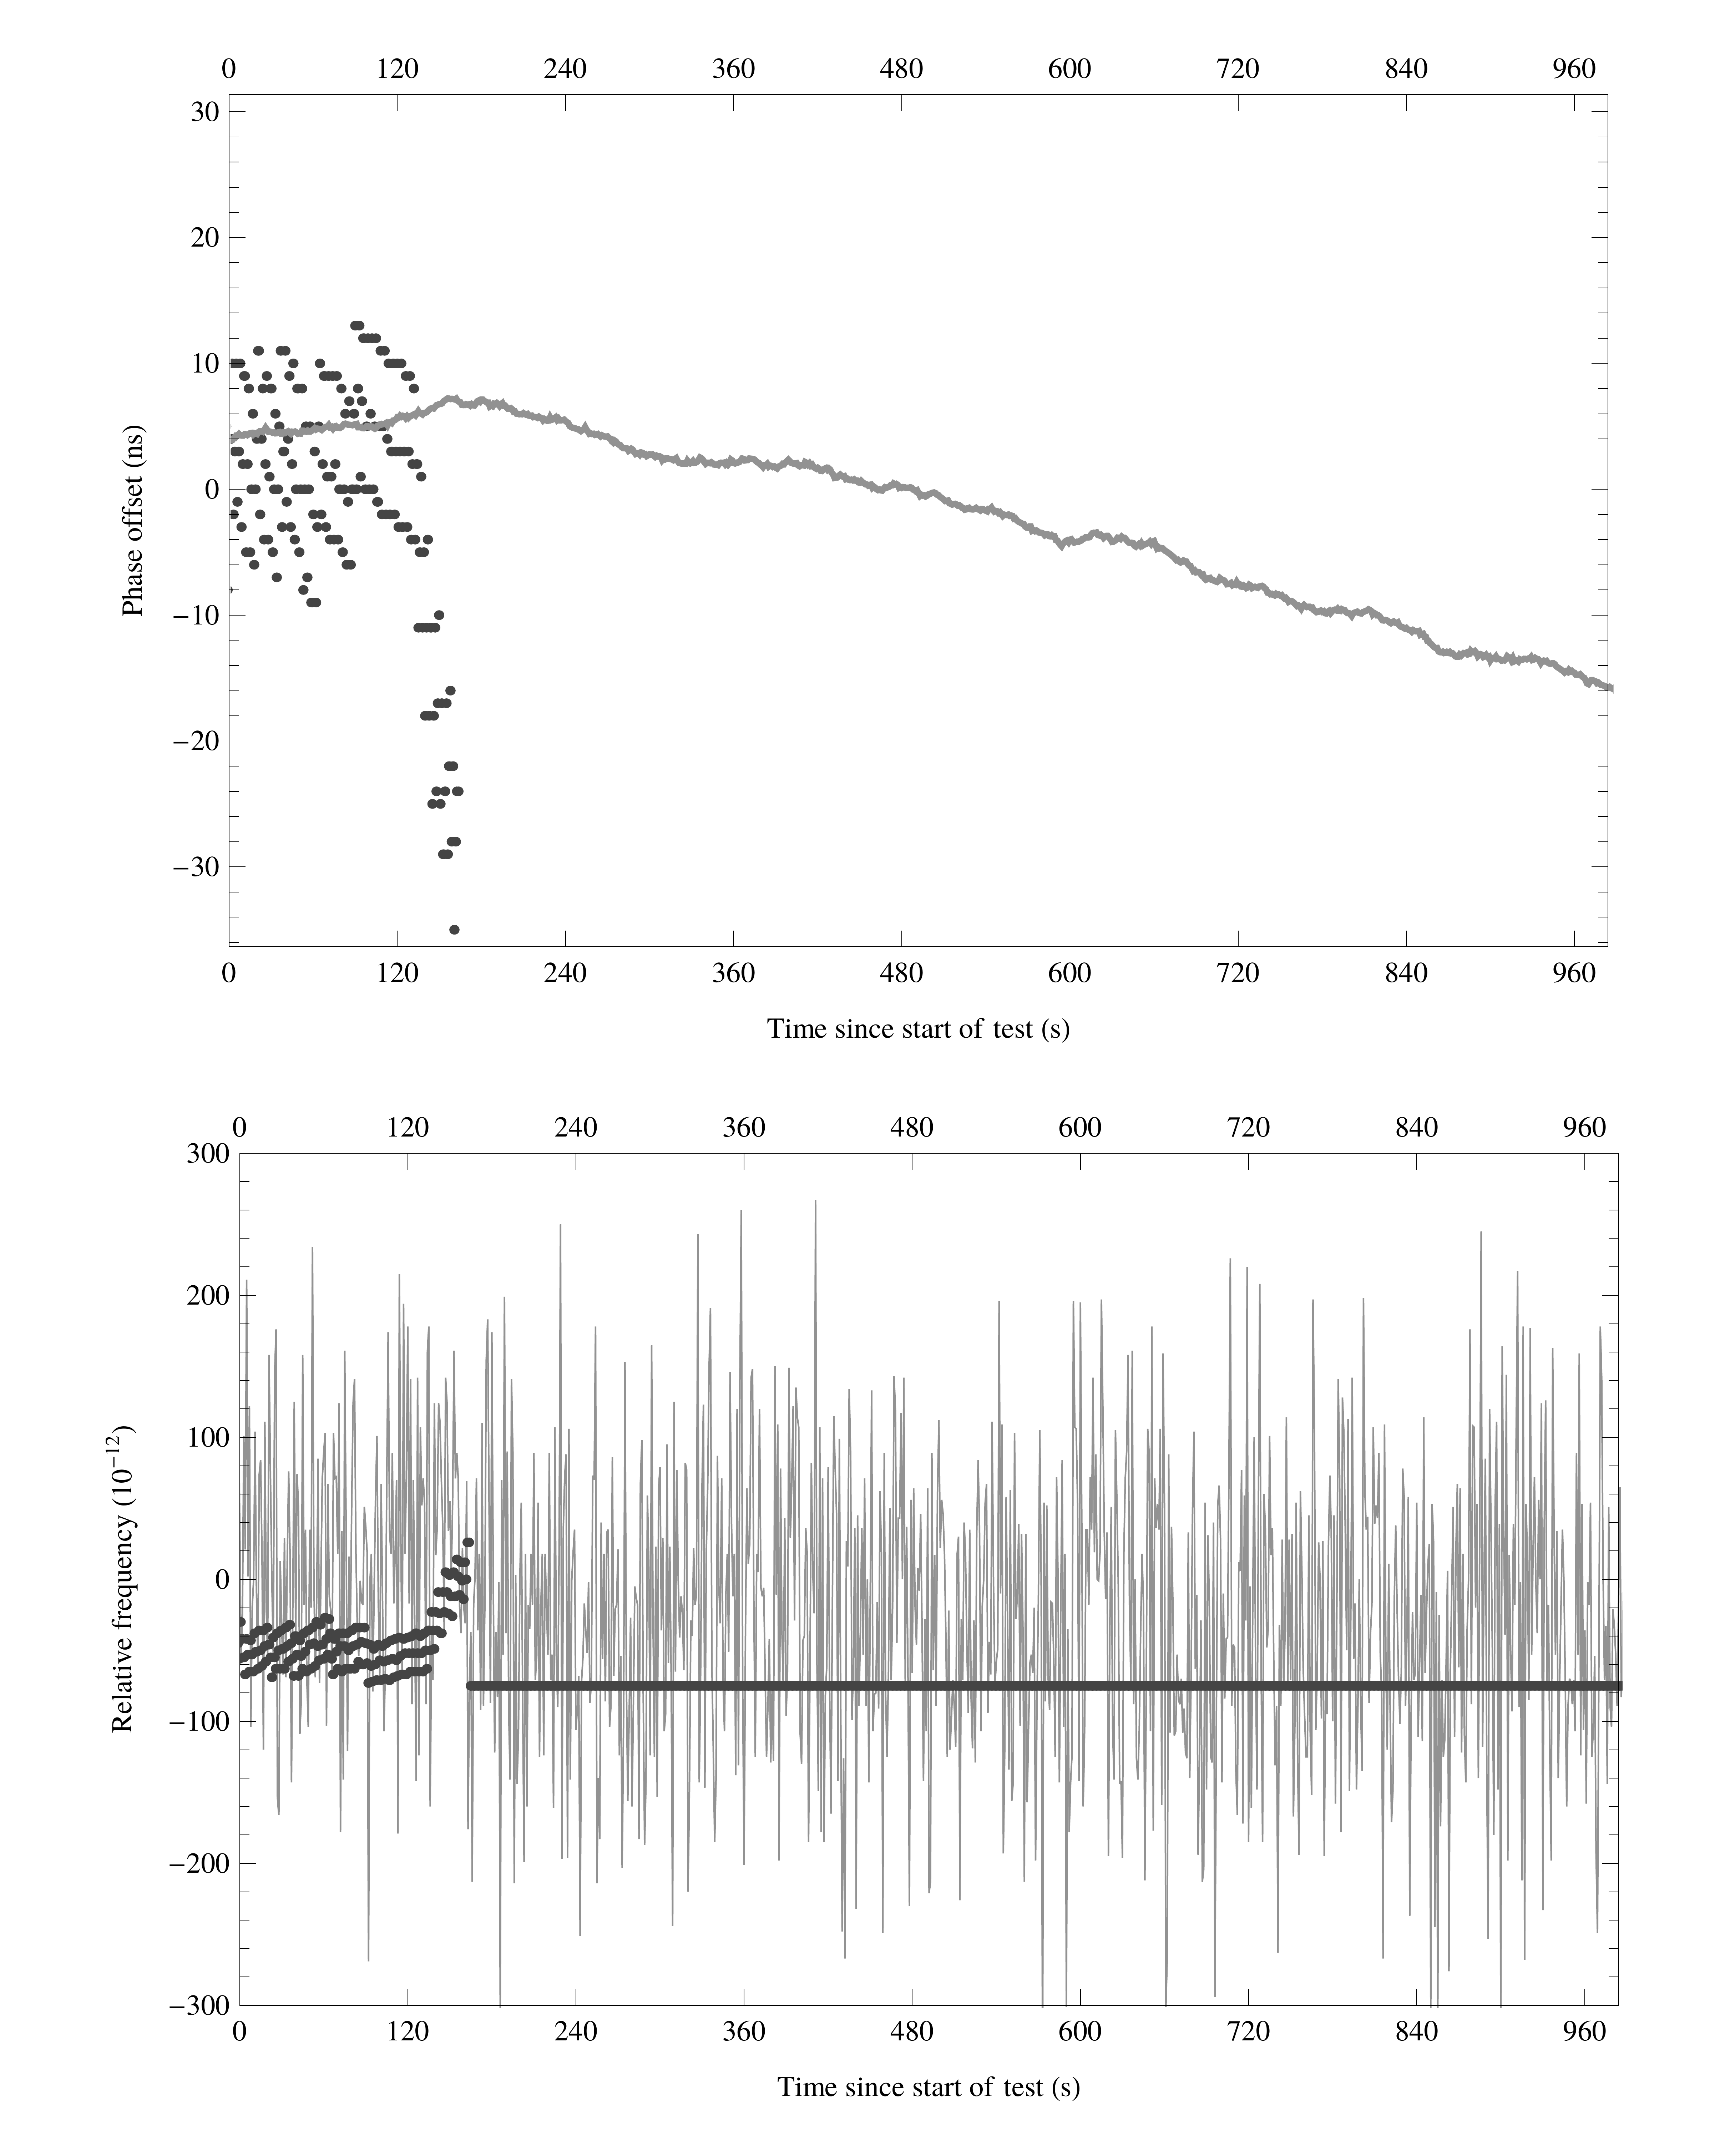
\includegraphics[width=1\textwidth]{20161024-test2-telemetry-and-cnt91-combined-1g.png}
  \caption{Timing measurements and clock telemetry data. The upper panel is phase offset in nanoseconds. The long, sloped light line is a plot of the measurements done by the CNT-91 frequency counter. The dotted dark plot, is also the phase offset but as reported by the atomic clock. The lighter plot in the background of the bottom panel is frequency steering as measured by the CNT-91 frequency counter. The dark plot is frequency offset as reported by the atomic clock.}
  \label{sensor2_measure}
\end{figure} 

\newpage
\section{Unplanned disturbance}\label{unplanned_disturb}
The data presented in this section was gathered while the atomic clock controller was building the clock model for one of the planned tests. The data is interesting because it shows a disturbance from an unknown source. The data shown in the figures are from the 5 October 2016 to 6 October 2016. Figure \ref{disturbance_holdover} shows that about 10 minutes after midnight on 6 October 2016, the atomic clock entered "holdover mode", indicating that the 1 PPS signal from the GPS receiver was lost. Figure \ref{disturbance_multipanel} shows the GPS receiver's solved altitude, longitude, latitude, speed and number of satellites. By examining the figure, it is obvious that the signal was lost minutes after the 57667 MJD (midnight) mark. The GPS receiver did not achieve consistent lock before approximately 57667.32 MJD (7:45 in the morning). In the meantime, the clock stability was impaired as figure \ref{disturbance_phase_frequency} and \ref{disturbance_phase_steer} clearly show. Figure \ref{disturbance_phase_steer} is interesting because it shows how the atomic clock seems to have a delay in its steering algorithm. If the atomic clock controller applied the clock model filters while this data was collected, the phase jump filter would have triggered before the atomic clock would have been able to apply steering. 

We have no idea what might be the origin of the disturbance. The following is therefore pure speculation: It is possible that a trucker spent the night parked by the road used a GPS jammer to hide his or her activities from an employer, and that the observed disturbance is a reflection of the jammer's signal. We did not find any traces of the disturbance when examining the logs from sensor one. Sensor one might have been shielded from a reflection because of its position. The time-frame for the disturbance also supports this theory since the disturbance started around midnight and ended at around 7:45, in other words "a good night sleep". This is of course only speculation as we do not have any data supporting it. 

\begin{figure}[!hbt]
  \centering
  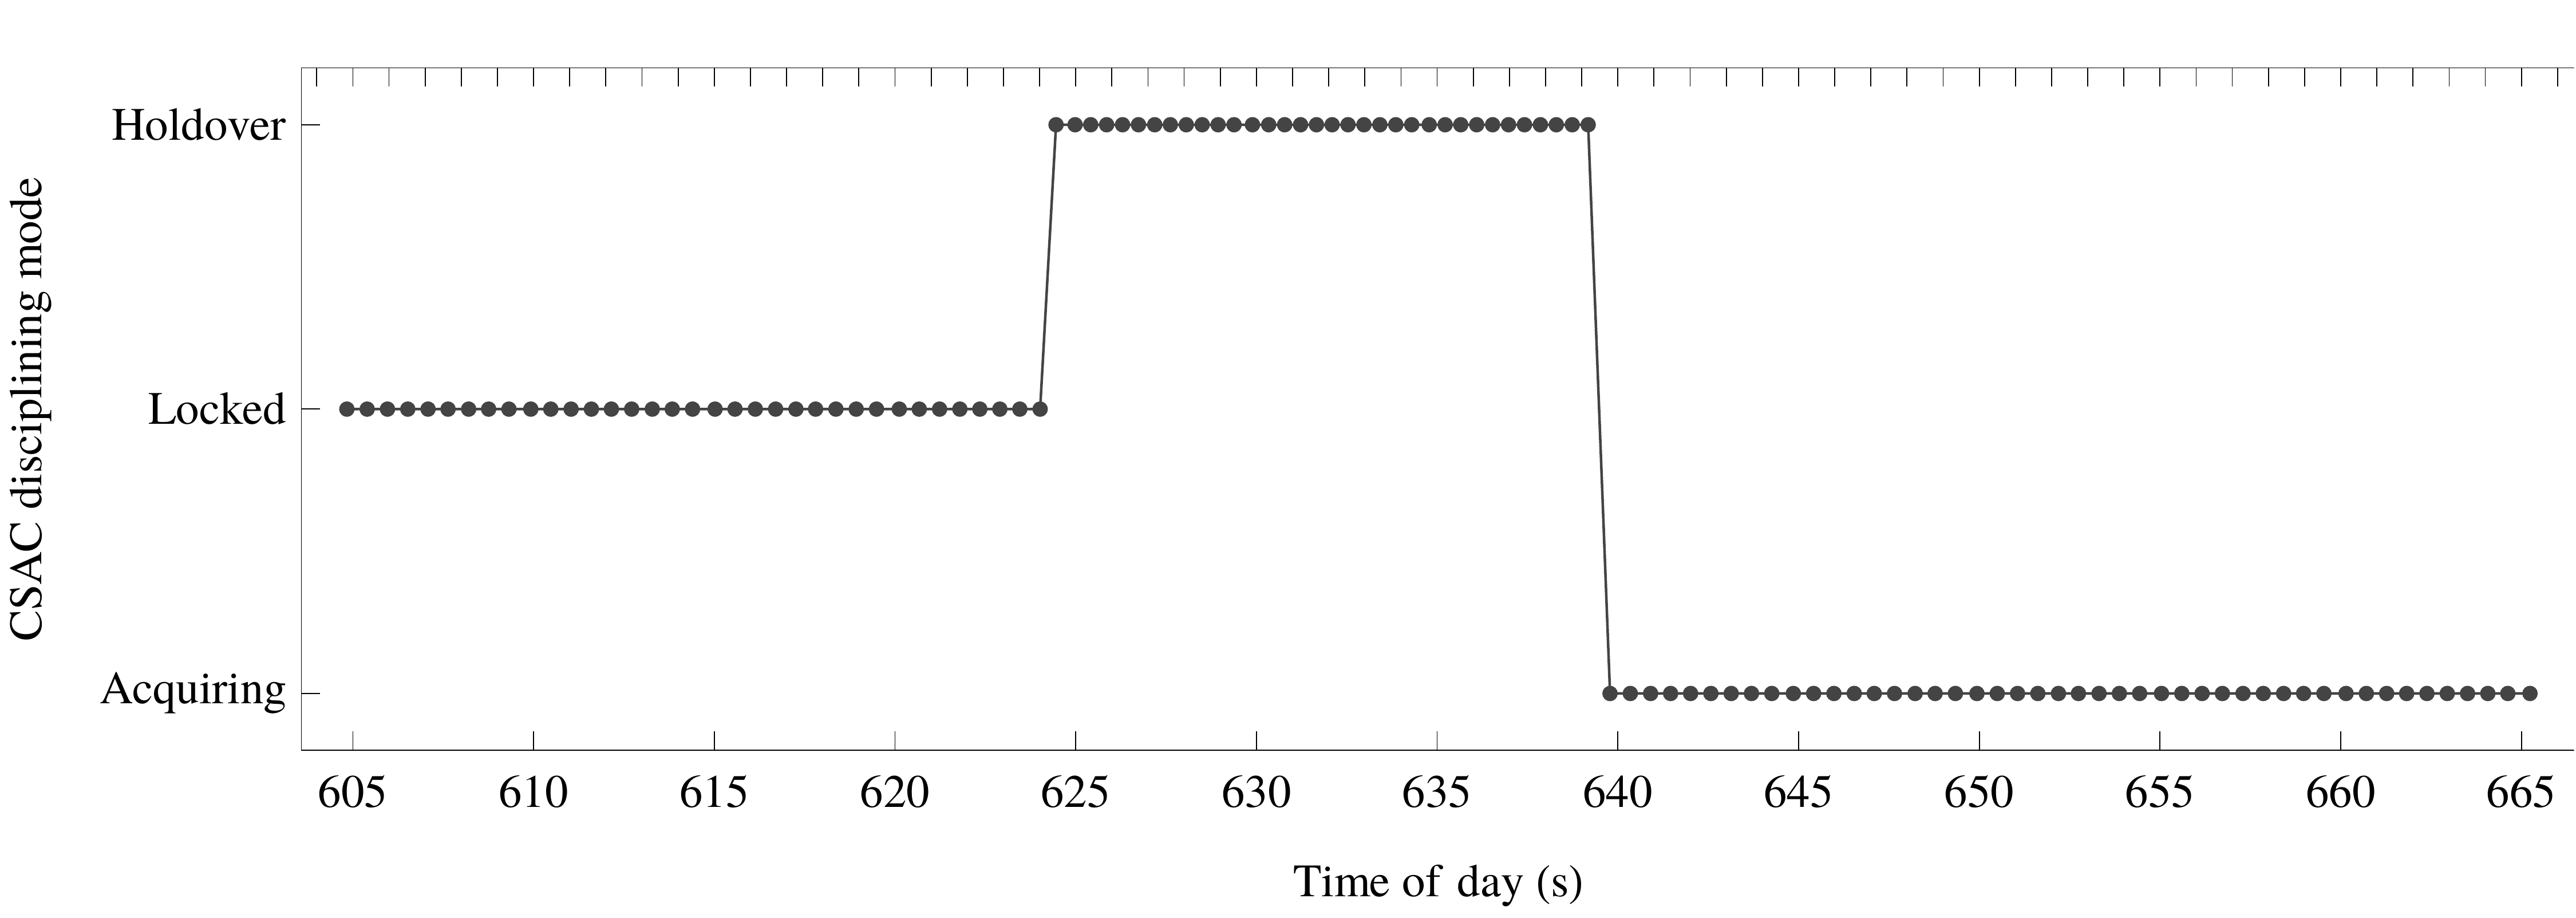
\includegraphics[width=1\textwidth]{disturbance57667-csac-telemetry-mode-zoom-in-1g.png}
  \caption{The figure shows the disciplined mode as reported by the atomic clock.}
  \label{disturbance_holdover}
\end{figure} 

\begin{figure}
  \centering
  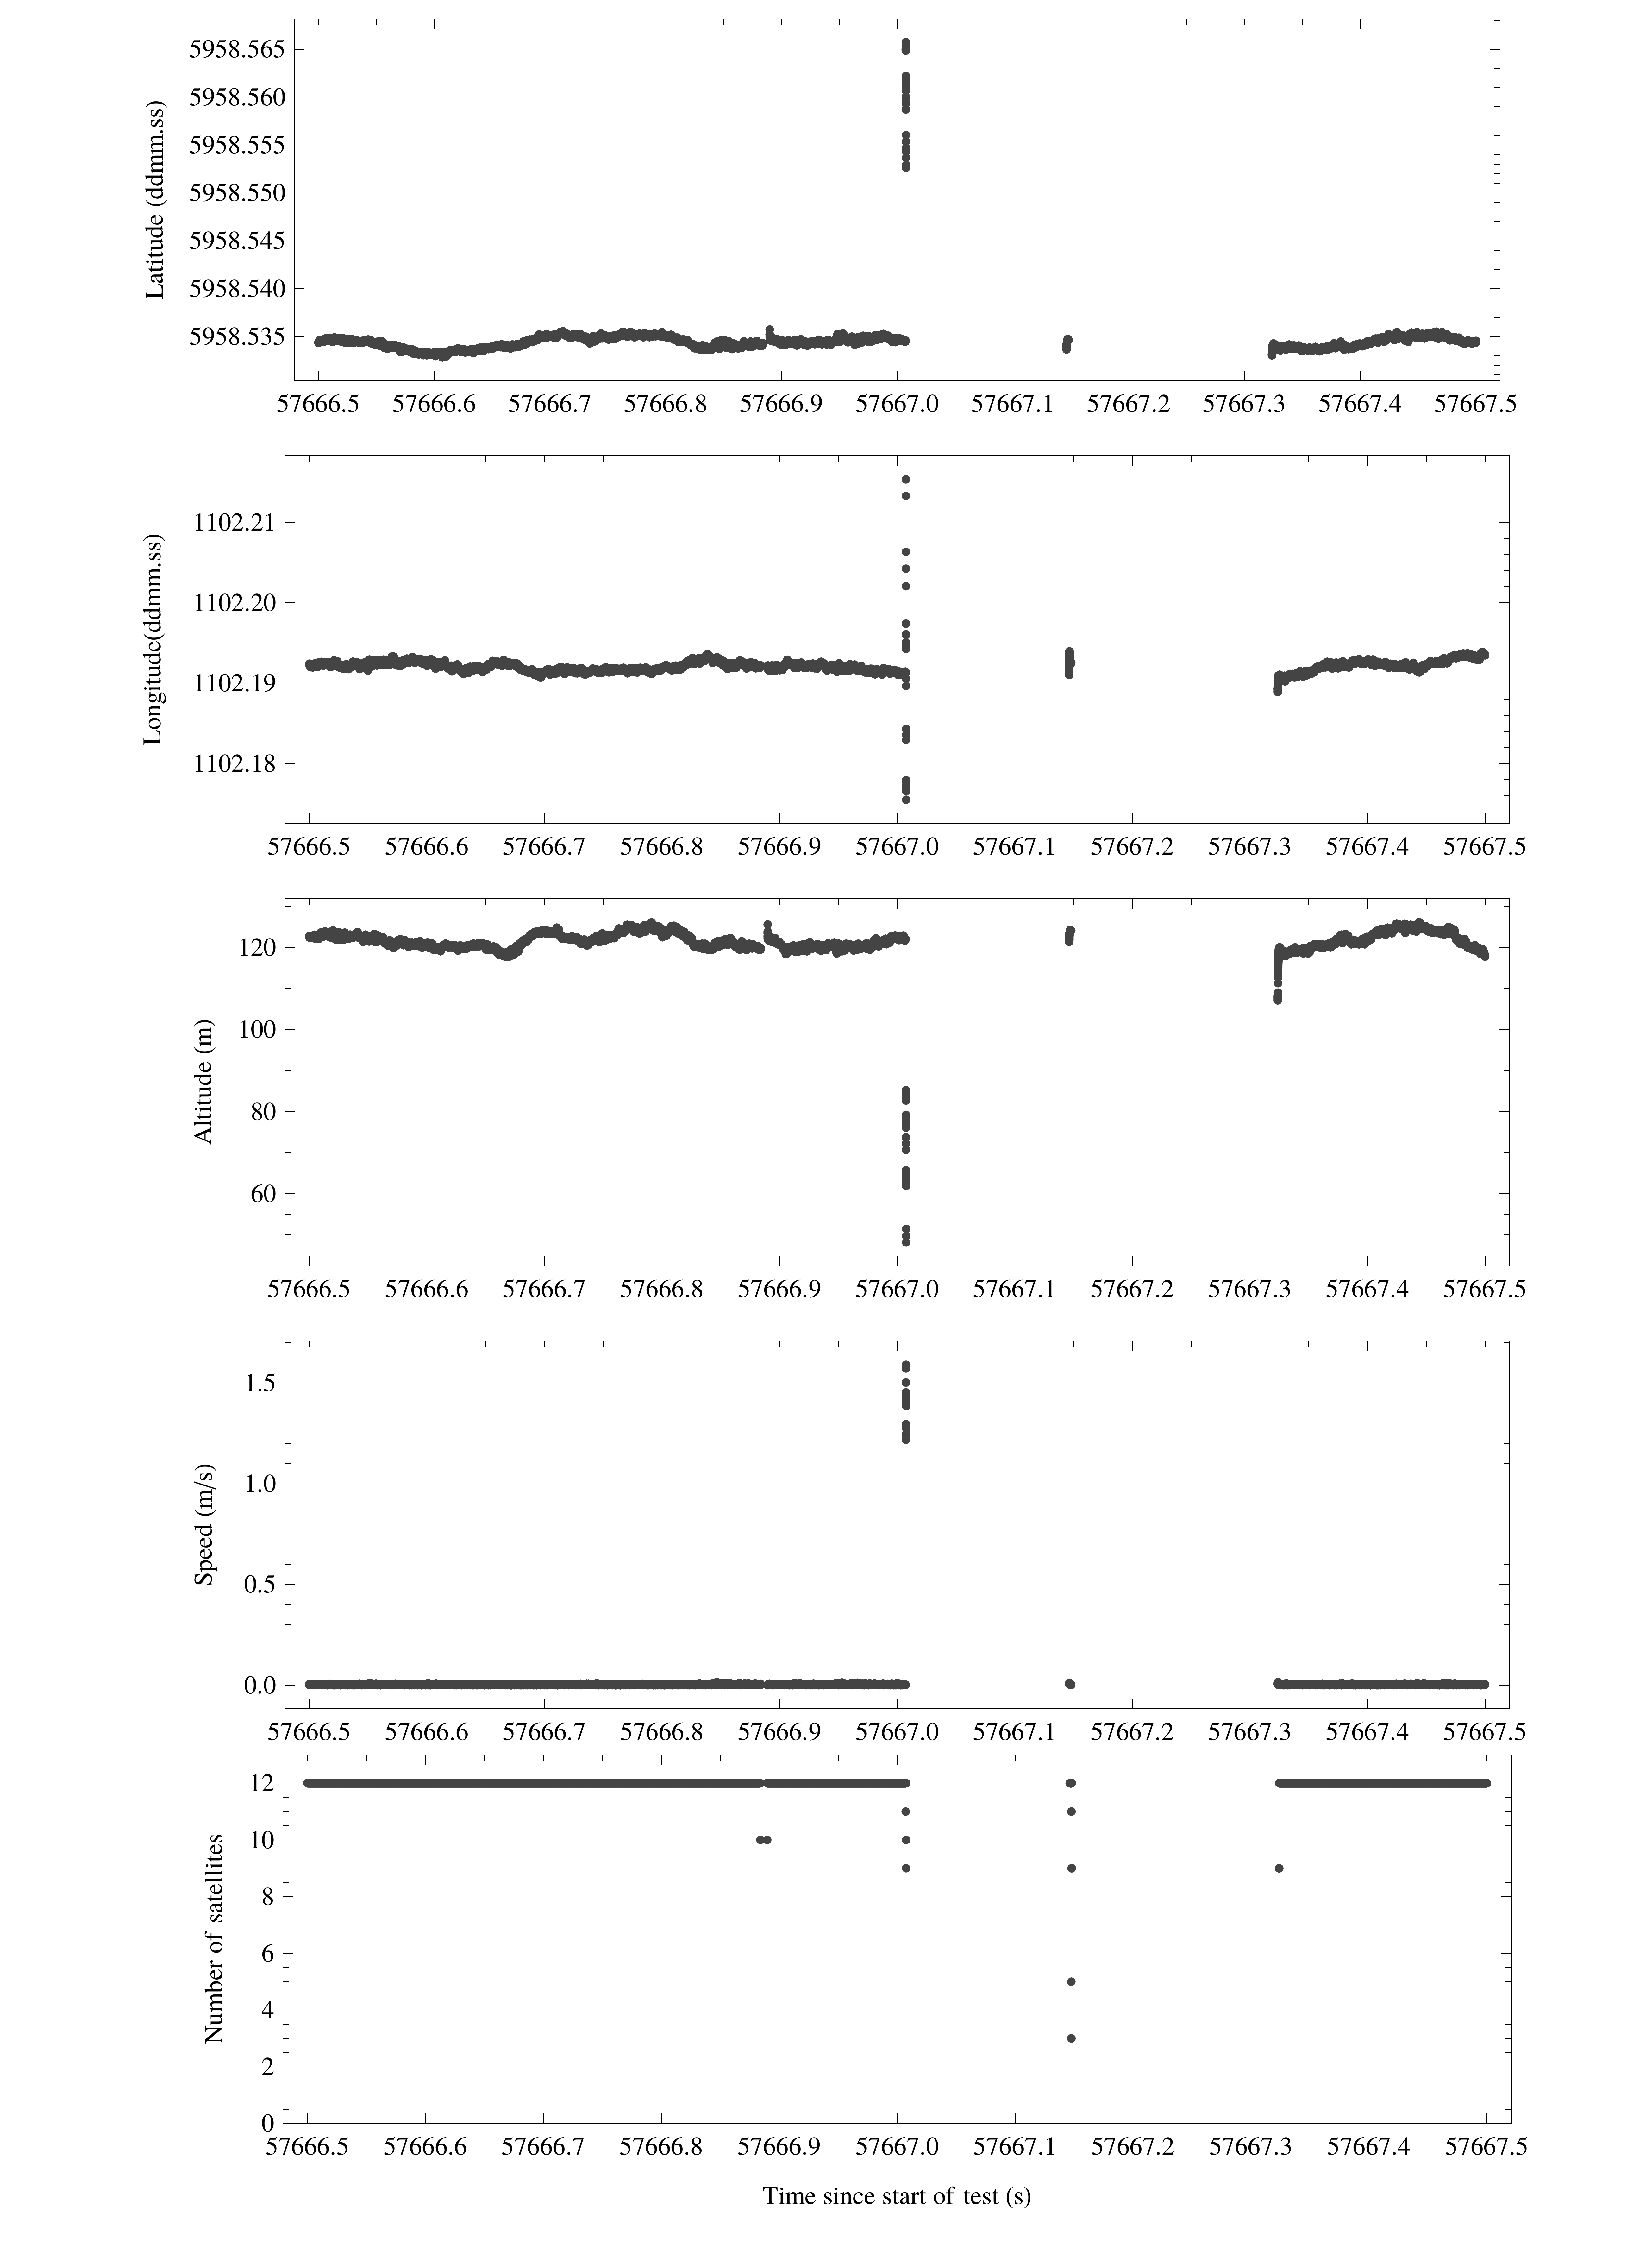
\includegraphics[width=1\textwidth]{disturbance57667-gps-sensor2-multipanel-1g.png}
  \caption{Figure shows solved position, speed and number of satellites as reported by the GPS receiver.}
  \label{disturbance_multipanel}
\end{figure}

\begin{figure}
  \centering
  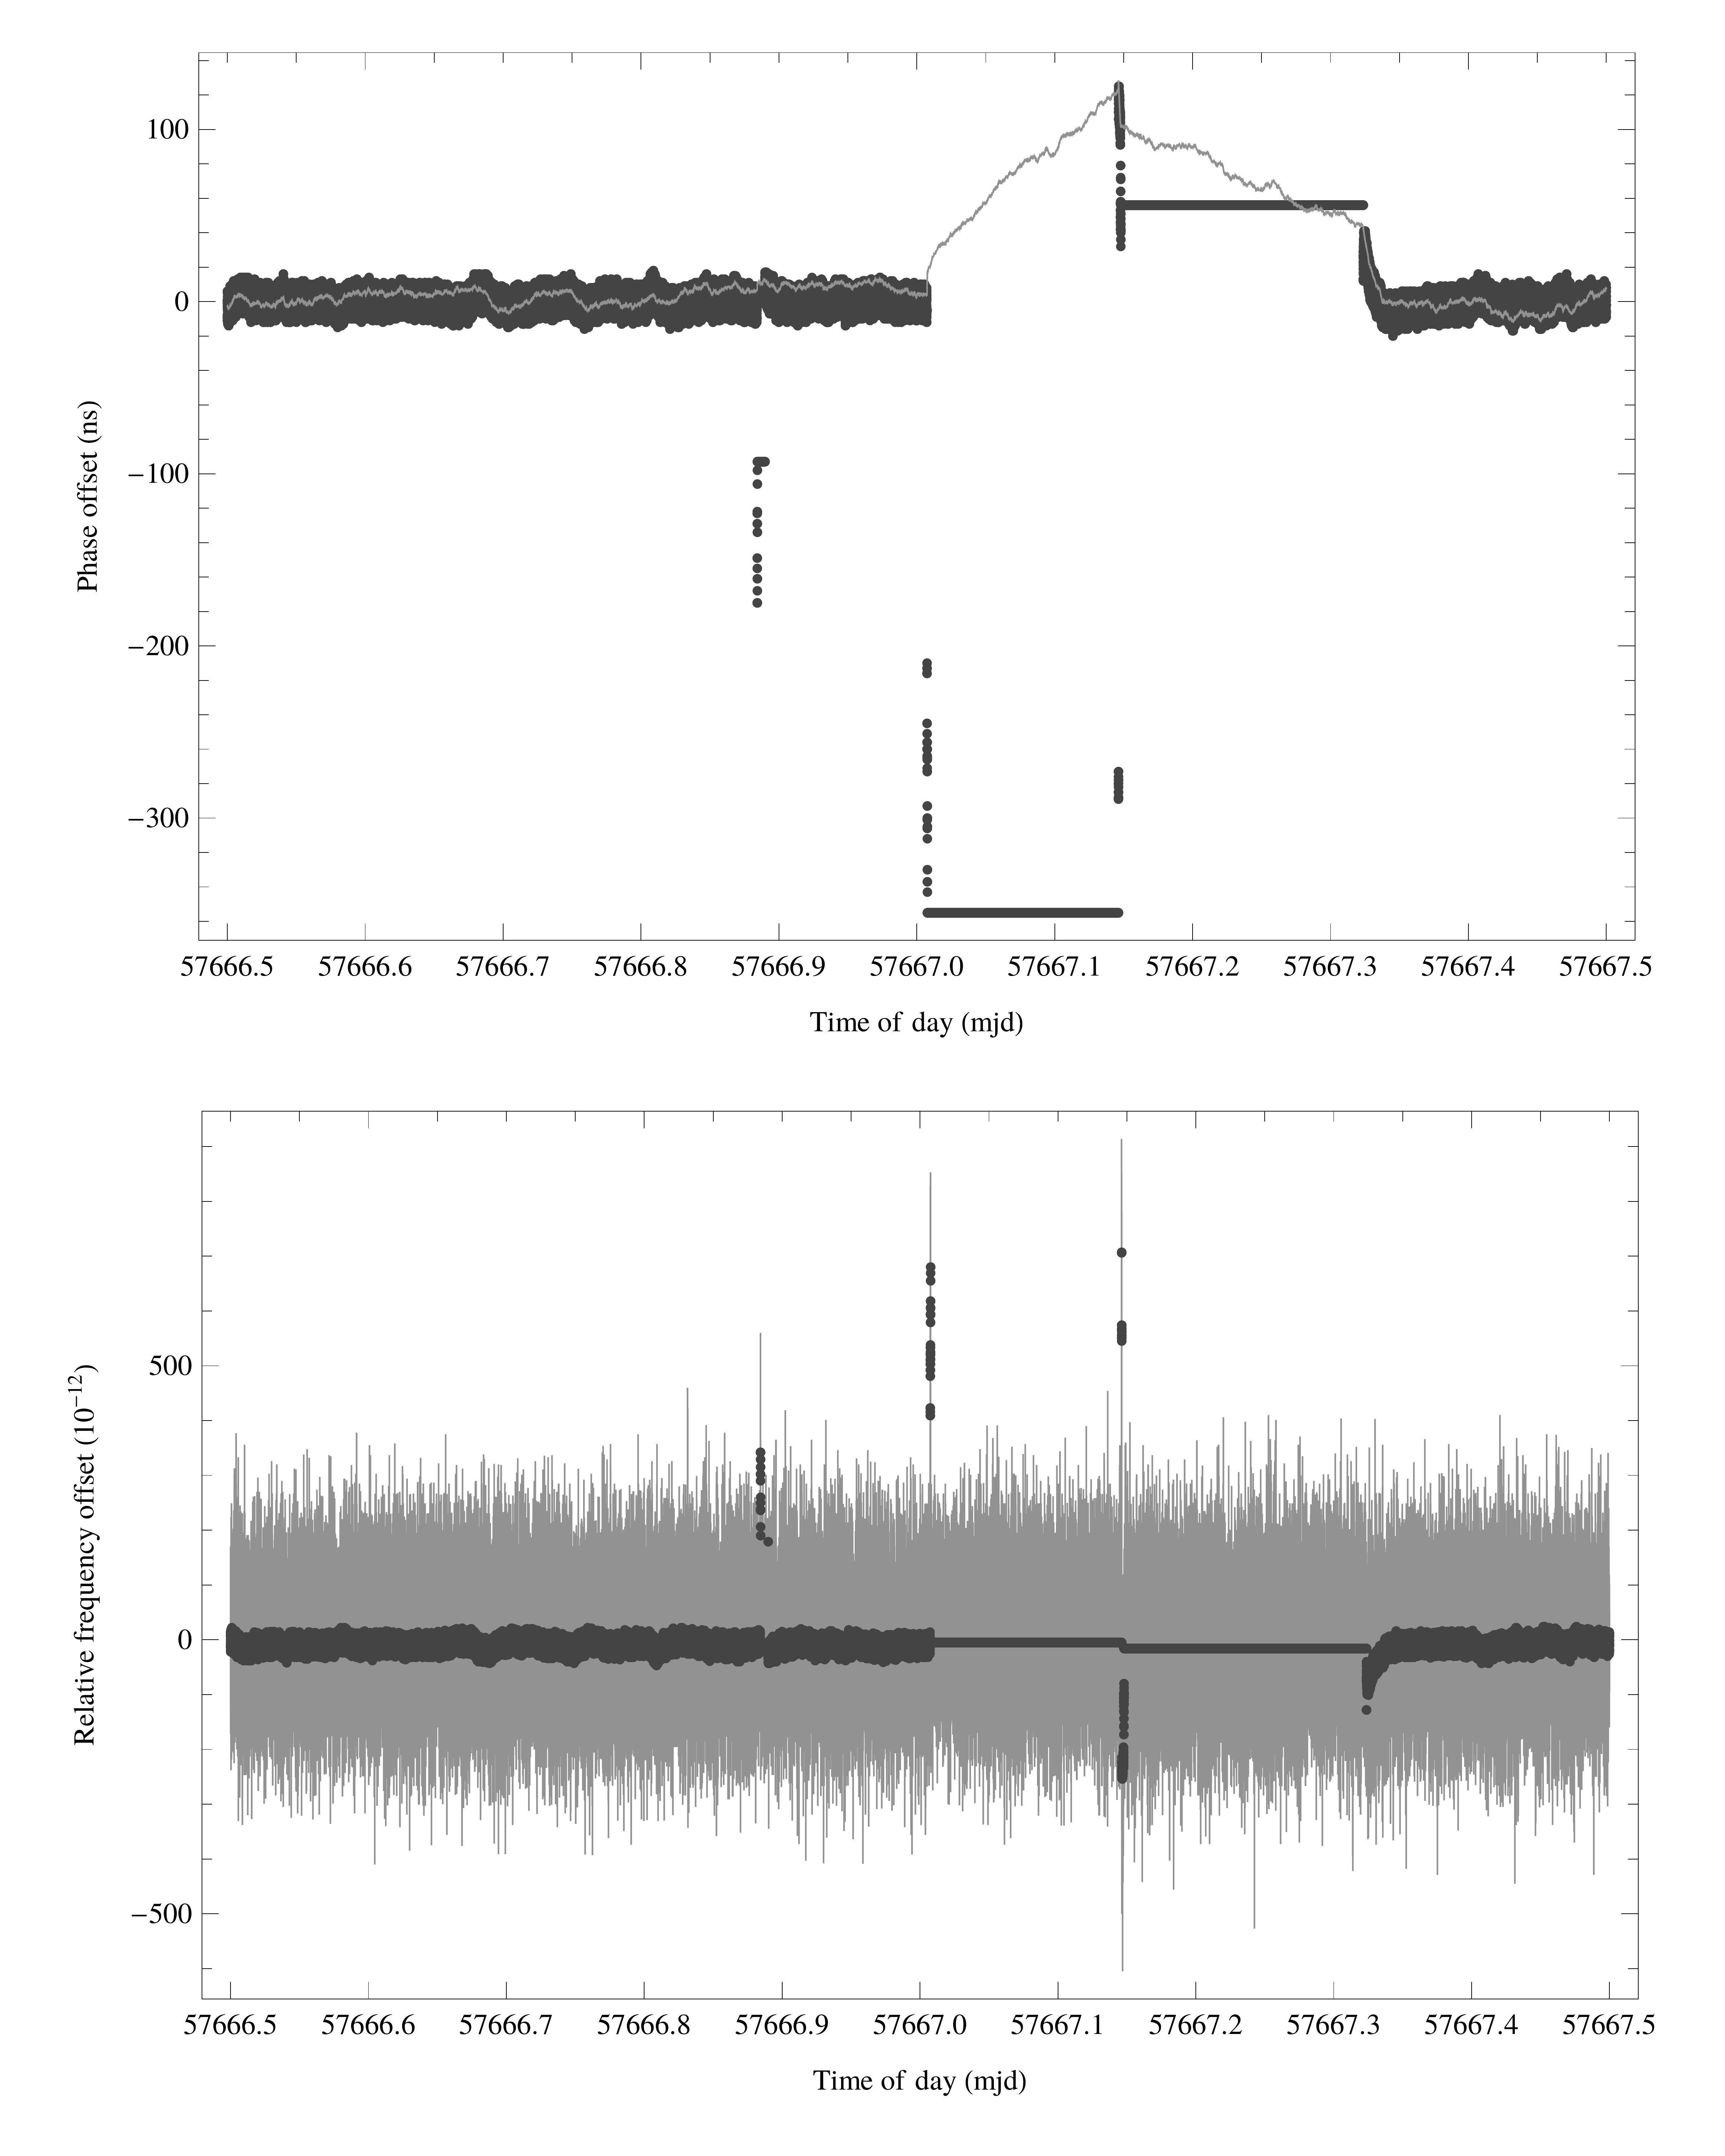
\includegraphics[width=1\textwidth]{disturbance57667-cnt91-csac-telemetry-phase-frequency-steer-combined-1g.png}
  \caption{Top figure shows phase offset in nanoseconds. The thin lightly colored line is as measured by the CNT-91 frequency counter. The solid darker line is from the telemetry string from the atomic clock.}
  \label{disturbance_phase_frequency}
\end{figure}

\begin{figure}
  \centering
  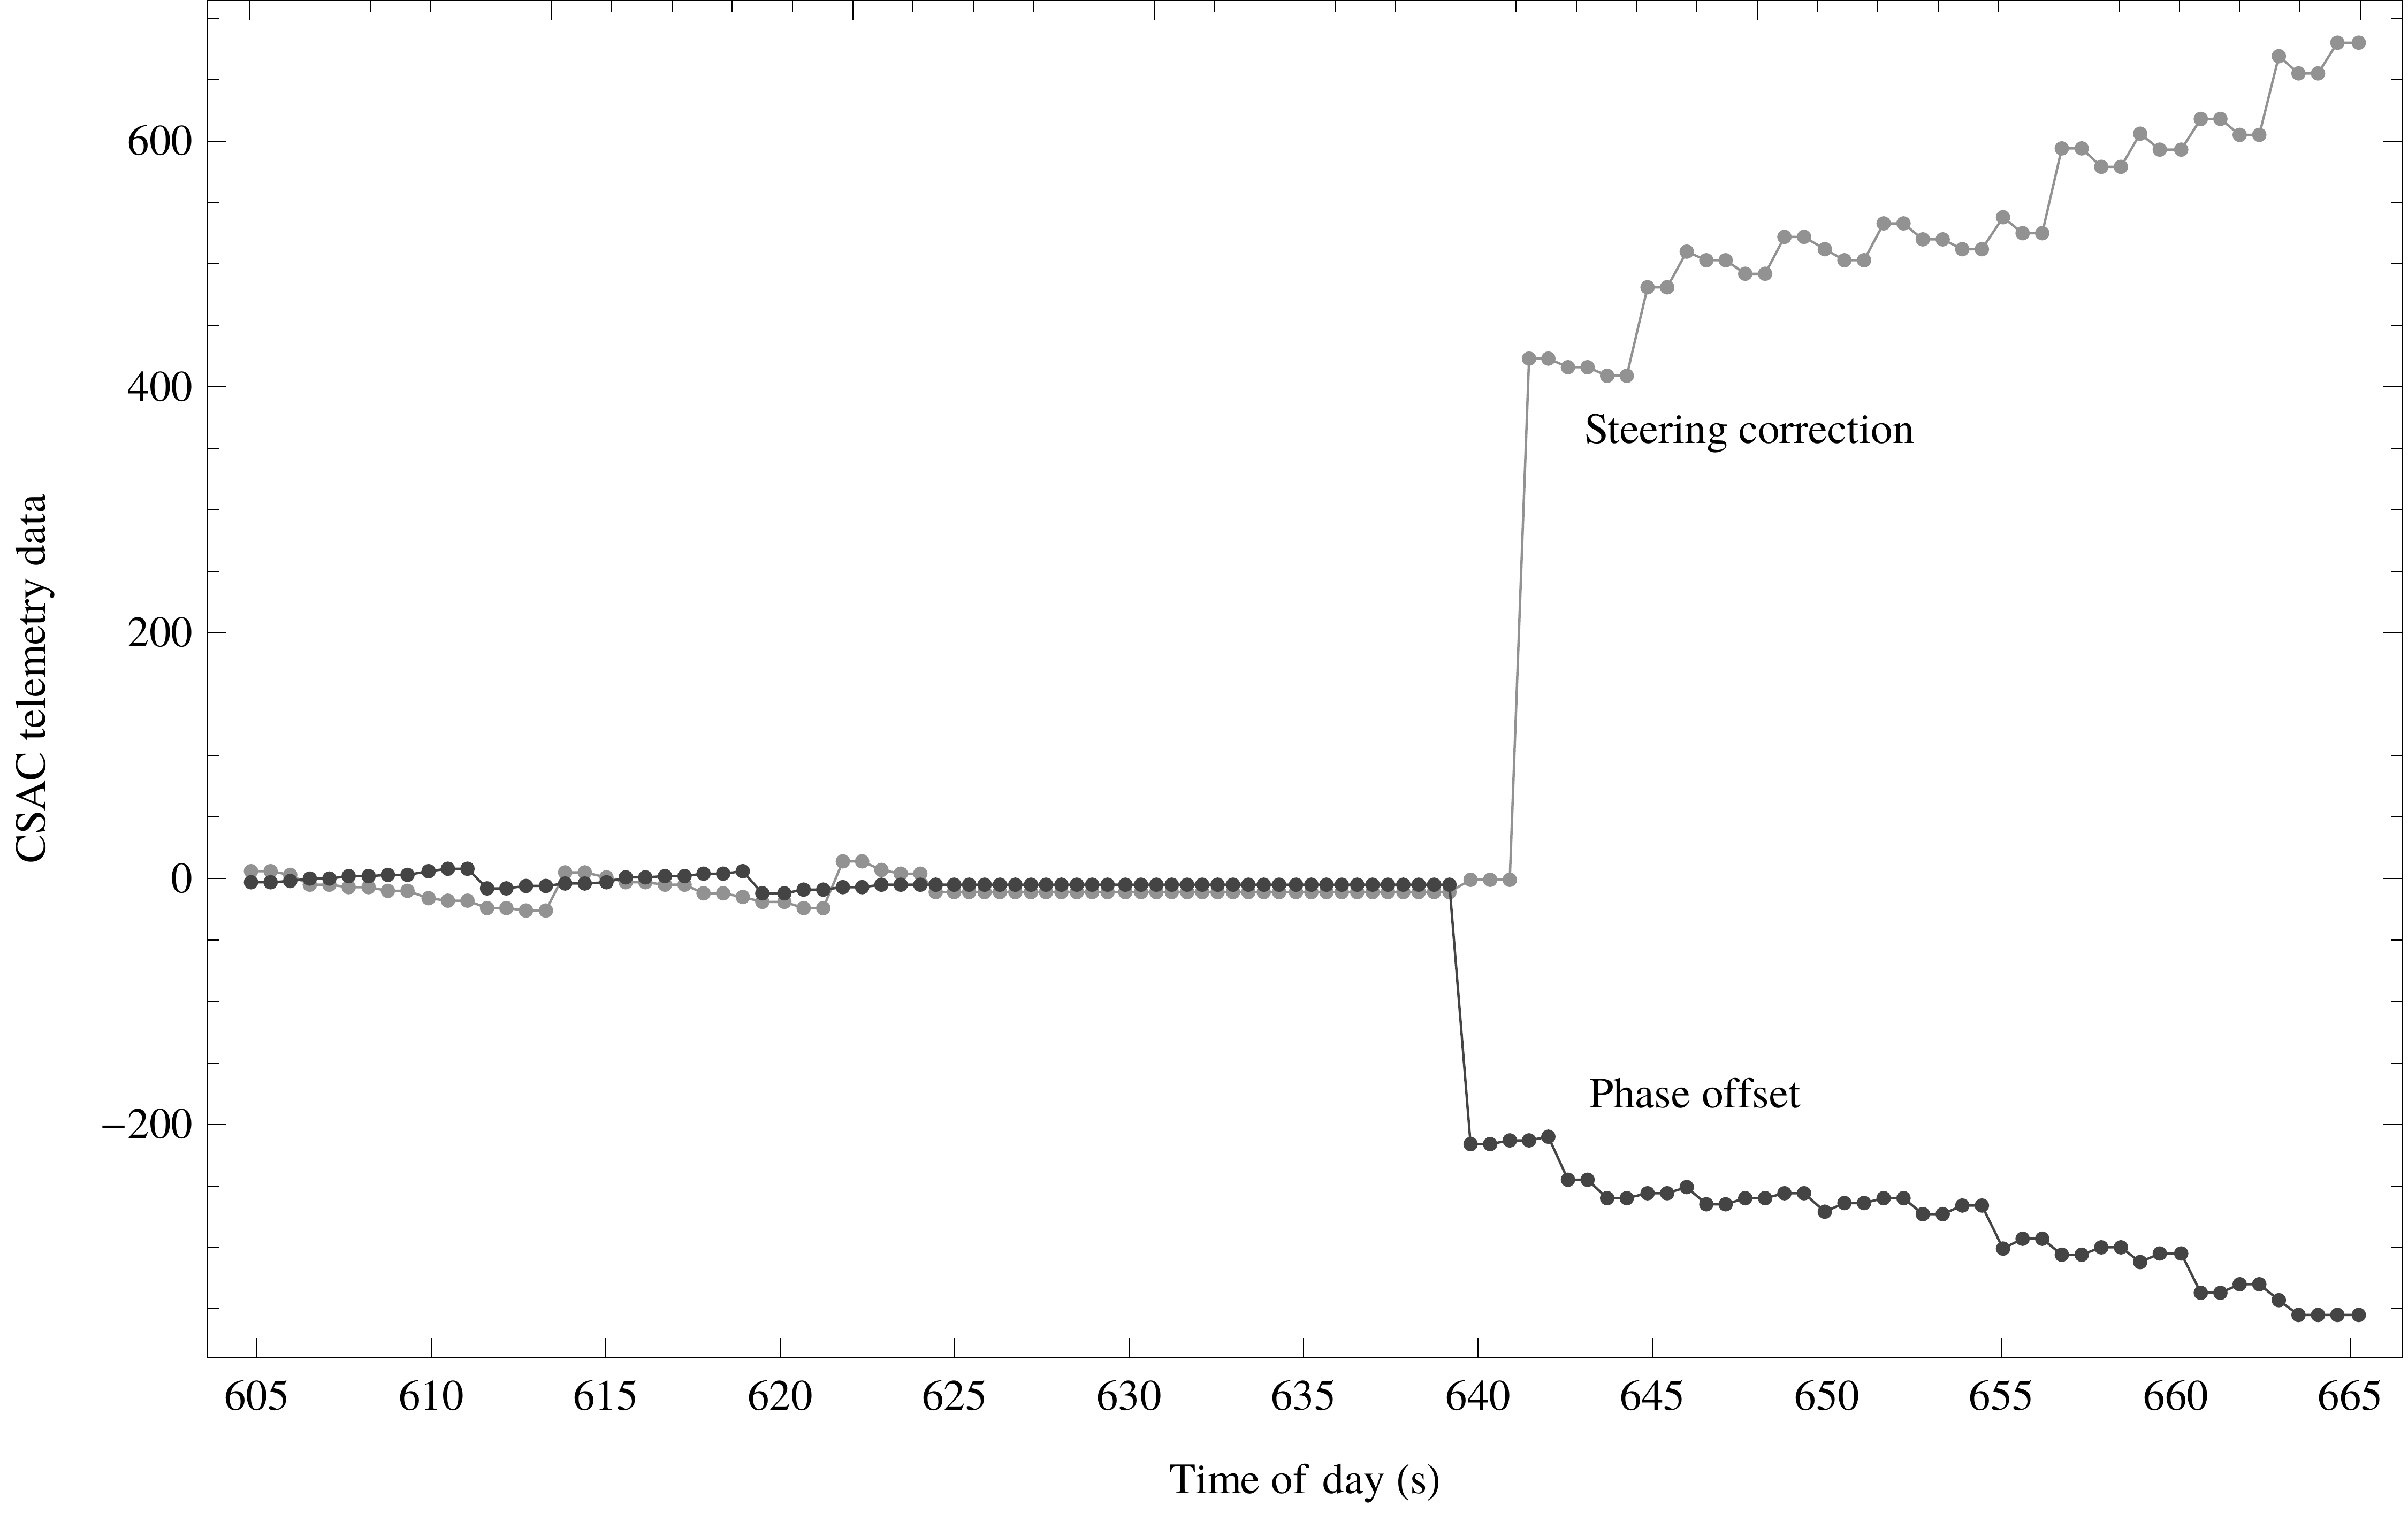
\includegraphics[width=1\textwidth]{disturbance57667-csac-telemetry-phase-steer-combined-zoom-in-2-1g.png}
  \caption{Figure shows the phase offset and steering correction as reported in the telemetry string from the atomic clock.}
  \label{disturbance_phase_steer}
\end{figure} 

 


